% Options for packages loaded elsewhere
\PassOptionsToPackage{unicode}{hyperref}
\PassOptionsToPackage{hyphens}{url}
%
\documentclass[
]{book}
\usepackage{lmodern}
\usepackage{amssymb,amsmath}
\usepackage{ifxetex,ifluatex}
\ifnum 0\ifxetex 1\fi\ifluatex 1\fi=0 % if pdftex
  \usepackage[T1]{fontenc}
  \usepackage[utf8]{inputenc}
  \usepackage{textcomp} % provide euro and other symbols
\else % if luatex or xetex
  \usepackage{unicode-math}
  \defaultfontfeatures{Scale=MatchLowercase}
  \defaultfontfeatures[\rmfamily]{Ligatures=TeX,Scale=1}
\fi
% Use upquote if available, for straight quotes in verbatim environments
\IfFileExists{upquote.sty}{\usepackage{upquote}}{}
\IfFileExists{microtype.sty}{% use microtype if available
  \usepackage[]{microtype}
  \UseMicrotypeSet[protrusion]{basicmath} % disable protrusion for tt fonts
}{}
\makeatletter
\@ifundefined{KOMAClassName}{% if non-KOMA class
  \IfFileExists{parskip.sty}{%
    \usepackage{parskip}
  }{% else
    \setlength{\parindent}{0pt}
    \setlength{\parskip}{6pt plus 2pt minus 1pt}}
}{% if KOMA class
  \KOMAoptions{parskip=half}}
\makeatother
\usepackage{xcolor}
\IfFileExists{xurl.sty}{\usepackage{xurl}}{} % add URL line breaks if available
\IfFileExists{bookmark.sty}{\usepackage{bookmark}}{\usepackage{hyperref}}
\hypersetup{
  pdftitle={Oscillations and Waves},
  pdfauthor={Dr.~Andrew McKinley},
  hidelinks,
  pdfcreator={LaTeX via pandoc}}
\urlstyle{same} % disable monospaced font for URLs
\usepackage{longtable,booktabs}
% Correct order of tables after \paragraph or \subparagraph
\usepackage{etoolbox}
\makeatletter
\patchcmd\longtable{\par}{\if@noskipsec\mbox{}\fi\par}{}{}
\makeatother
% Allow footnotes in longtable head/foot
\IfFileExists{footnotehyper.sty}{\usepackage{footnotehyper}}{\usepackage{footnote}}
\makesavenoteenv{longtable}
\usepackage{graphicx,grffile}
\makeatletter
\def\maxwidth{\ifdim\Gin@nat@width>\linewidth\linewidth\else\Gin@nat@width\fi}
\def\maxheight{\ifdim\Gin@nat@height>\textheight\textheight\else\Gin@nat@height\fi}
\makeatother
% Scale images if necessary, so that they will not overflow the page
% margins by default, and it is still possible to overwrite the defaults
% using explicit options in \includegraphics[width, height, ...]{}
\setkeys{Gin}{width=\maxwidth,height=\maxheight,keepaspectratio}
% Set default figure placement to htbp
\makeatletter
\def\fps@figure{htbp}
\makeatother
\setlength{\emergencystretch}{3em} % prevent overfull lines
\providecommand{\tightlist}{%
  \setlength{\itemsep}{0pt}\setlength{\parskip}{0pt}}
\setcounter{secnumdepth}{5}
\usepackage{booktabs}
\usepackage{amsthm}
\makeatletter
\def\thm@space@setup{%
  \thm@preskip=8pt plus 2pt minus 4pt
  \thm@postskip=\thm@preskip
}
\makeatother
\usepackage[]{natbib}
\bibliographystyle{apalike}

\title{Oscillations and Waves}
\author{Dr.~Andrew McKinley}
\date{2021-03-09}

\begin{document}
\maketitle

{
\setcounter{tocdepth}{1}
\tableofcontents
}
\hypertarget{welcome}{%
\chapter*{Welcome}\label{welcome}}
\addcontentsline{toc}{chapter}{Welcome}

Welcome to the course notes for the Oscillations and Waves component of PHYS10005, Core Physics II.

The most recent version of these notes can be found at \url{https://awmckinley1.github.io/osc-waves1}

\hypertarget{about-these-notes}{%
\section*{About these notes}\label{about-these-notes}}
\addcontentsline{toc}{section}{About these notes}

These notes have been prepared in a format which maintains compatibility with screen-readers, while also allowing the facility for both PDF and EPUB downloads for those who wish to use them.

The HTML also has themes to facilitate easier reading (font colours, serif/sans serif fonts etc.). Please explore the top bar of the web environment to explore this.

The HTML notes allow for embedding of rich content (videos, animations, etc.), and for this reason I recommend accessing the course using the web-links provided, as these cannot be included in static PDF or EPUB documents. However, I will ensure links are included in these formats as far as possible.

These notes are a ``live document'', and as such they can (and will) be updated should any erroneous explanations be found or additional explanations be needed. For this reason, please do email me if you have any questions or if anything is not clear.

The most recent version can always be found at the link at the top of this section, and any changes are reflected in the change-log (\ref{sec:changelog})

Please note that as this is a ``live document'', a downloaded version can become obsolete. Please refer back regularly and refer to the changelog for any updates.

\hypertarget{error-reporting}{%
\section*{Error reporting}\label{error-reporting}}
\addcontentsline{toc}{section}{Error reporting}

As much as we try, sometimes errors creep in. At best, it is little more than a careless typo which makes the reader tut with disappointment, at worst it risks seriously misleading the learner. For this reason I have created a feedback form to report errors; this is accessible at the bottom of this page.

\hypertarget{course-history}{%
\section*{Course history}\label{course-history}}
\addcontentsline{toc}{section}{Course history}

This iteration of the course has been written for the academic year 2020/21 by Andrew McKinley. This has been based extensively on previous course notes by Ben Maughan, Simon Hanna and Massimo Antognozzi.

\hypertarget{sec:changelog}{%
\section*{Changelog}\label{sec:changelog}}
\addcontentsline{toc}{section}{Changelog}

2021-03-07 Updated to address error reports, added additional detail for figures in Chapter 11, and including images for chapter 13

2021-02-14 Updated to address error reports, and to include images and additional explanations for Chapters 10 and 11.

2021-02-12 Updated to address error reports 1-13. Thank you all who sent them in.

2021-01-27 Initial commit to GitHub; all text for the course complete, some images pending.

2020-09-16 Initial versioning and inclusion of course material.

\hypertarget{report-an-error}{%
\section*{Report an error}\label{report-an-error}}
\addcontentsline{toc}{section}{Report an error}

Direct link to error reporting form (opens in new window)

Embedded form:

\hypertarget{sec:shm}{%
\chapter{Simple Harmonic Motion}\label{sec:shm}}

Simple harmonic motion (SHM) is a simple and common type of oscillatory motion. It is a model which is widely used in modelling systems due to its simplicity.

In general, an object will move under SHM where its acceleration is:

\begin{enumerate}
\def\labelenumi{\arabic{enumi}.}
\tightlist
\item
  proportional to its displacement, but
\item
  in the opposite direction.
\end{enumerate}

The force causing this acceleration is often termed a \emph{restoring force} as it acts to push the object back to its starting point.

\hypertarget{sec:ch1-simpleshmexample}{%
\section{A simple example of SHM}\label{sec:ch1-simpleshmexample}}

Consider a block on a spring (Figure \ref{fig:ch1-blockonspring1})

\begin{figure}

{\centering 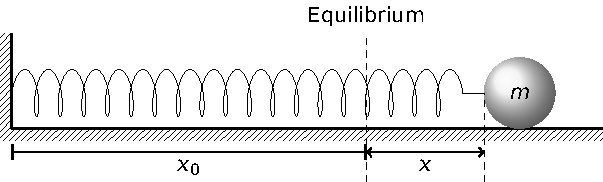
\includegraphics[width=0.7\linewidth]{visualisations/LaTeX/ch1-blockonspring1} 

}

\caption{A mass on a spring, stretched distance $x$ past its equilibrium length $x_0$}\label{fig:ch1-blockonspring1}
\end{figure}

By Hooke's law, the spring exerts a force on the block proportional to its displacement \(x\), but in the opposite direction, pushing the block back to its equilbrium position, shown mathematically in Equation \eqref{eq:hookeslaw1}:

\begin{equation}
F_x = -kx
\label{eq:hookeslaw1}
\end{equation}

In this example, \(F_x\) is considered a \textbf{restoring force}, while \(k\) is the force constant of the spring.

Applying Newton's Second Law to this problem, we can obtain the mathematical description of the system:

\begin{equation}
\begin{aligned}
F_x = ma_x \\
-kx = m\frac{\textrm{d}^2 x}{\textrm{d} t^2}
\end{aligned}
\end{equation}

\ldots{} and through rearrangement and combination with Equation \eqref{eq:hookeslaw1} we obtain the description of how this mass will move (Equation \eqref{eq:shm-massonspring1}):

\begin{equation}
\frac{\textrm{d}^2 x}{\textrm{d} t^2} = -\frac{k}{m}x
\label{eq:shm-massonspring1}
\end{equation}

The general form of this expresssion for any system can be considered as shown in Equation \eqref{eq:shm-general-massonspring1}

\begin{equation}
\frac{\textrm{d}^2 x}{\textrm{d} t^2} = -Cx \quad\mathrm{or}\quad\ddot{x} = -Cx
\label{eq:shm-general-massonspring1}
\end{equation}

\ldots where \(C\) is a positive constant which depends on the system and represents a ratio of the elastic (\(k\)) and inertial (\(m\)) contributions within the system.

\hypertarget{key-terms}{%
\subsection{Key terms}\label{key-terms}}

\begin{itemize}
\tightlist
\item
  \textbf{Period}: The time \(T\) for one complete oscilation back and forth (units s)
\item
  \textbf{Frequency}: The reciprocal of the period; \(f = \frac{1}{T}\), units s\textsuperscript{-1} or Hz.
\end{itemize}

\hypertarget{sec:shm-position}{%
\section{Positioning in SHM}\label{sec:shm-position}}

SHM can be described by a general equation of motion, defining the position (\(x\)) of the oscillating mass using a cosine function (Equation \eqref{eq:shm-general-positionx1})

\begin{equation}
x = A \cos (\omega t + \delta)
\label{eq:shm-general-positionx1}
\end{equation}

The parameters in this equation are:

\begin{itemize}
\tightlist
\item
  \(A\): The amplitude of the oscillation
\item
  \(\omega t + \delta\): Phase of motion
\item
  \(\delta\): Phase constant
\end{itemize}

For any single oscillator, the time origin can always be chosen so that \(\delta = 0\). For two or more oscillators there will generally be a phase difference between them (\emph{i.e.} they will not always be at the same `zero' position at time zero - Figure \ref{fig:ch1-shmpos-1})

\textbf{Figure of position vs time for two oscilators}

\begin{figure}

{\centering 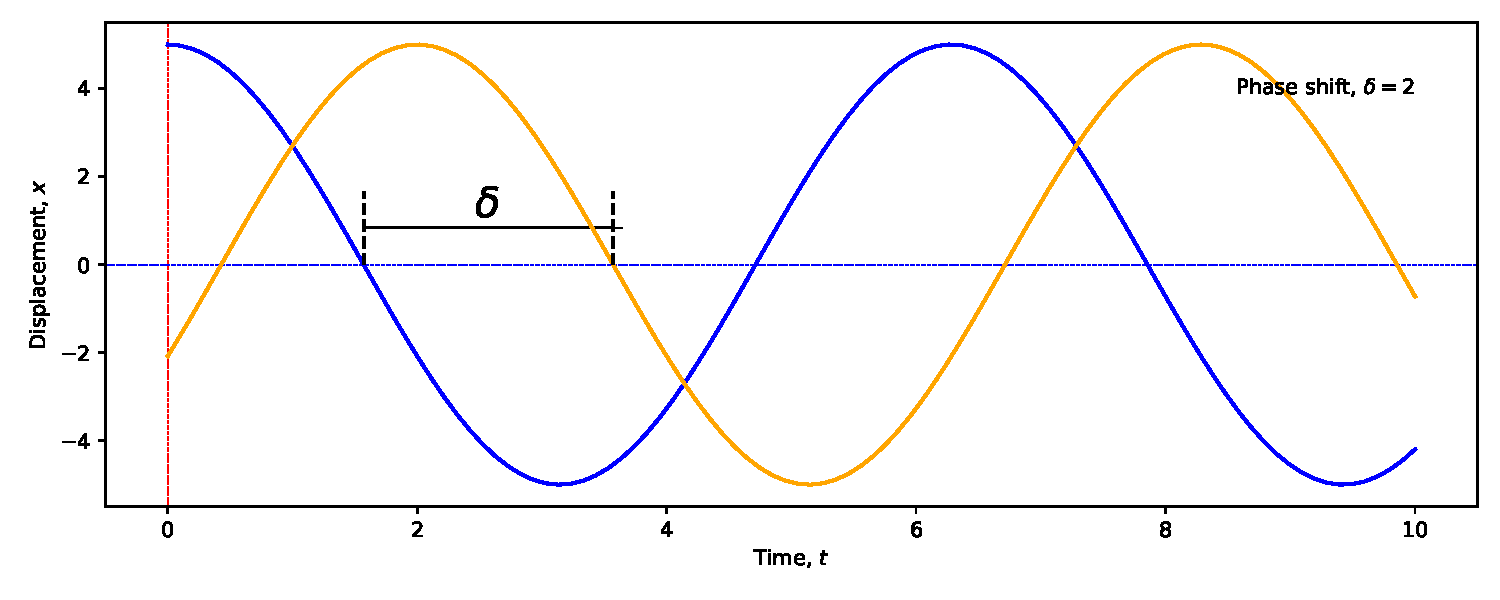
\includegraphics[width=0.7\linewidth]{visualisations/ch1-shmpos} 

}

\caption{An illustration of the changing position of two oscillators with respect to time, with a relative phase shift of 2 radians. }\label{fig:ch1-shmpos-1}
\end{figure}

\hypertarget{sec:shm-velocity}{%
\section{Velocity in SHM}\label{sec:shm-velocity}}

To find the velocity of the oscillating mass, we can simply find the first derivative of its position with respect to time (Equation \eqref{eq:shm-general-velocityx1}):

\begin{equation}
\begin{array}{rcl}
v & = & \frac{\textrm{d}x}{\textrm{d}t}\\
&=& -A \omega \sin (\omega t + \delta)\\
\end{array}
\label{eq:shm-general-velocityx1}
\end{equation}

A quick inspection of this shows that the velocity \(v\) is maximised when \(x\) is at a minimum; \emph{i.e.} as the object passes through its equilibirum position.

\hypertarget{sec:shm-acceleration}{%
\section{Acceleration in SHM}\label{sec:shm-acceleration}}

Again, to find the acceleration, we find the second derivative of its position with respect to time (Equation \eqref{eq:shm-general-accelerationx1}):

\begin{equation}
\begin{array}{rcl}
a & = & \frac{\textrm{d}v}{\textrm{d}t} = \frac{\textrm{d}^2 x}{\textrm{d}t^2}\\
&=& -A \omega^2 \cos (\omega t + \delta)\\
\end{array}
\label{eq:shm-general-accelerationx1}
\end{equation}

\ldots or, to use the Newtonian ``dot'' notation (Equation \eqref{eq:shm-general-accelerationx2}):

\begin{equation}
a = \ddot{x} = -\omega^2 x
\label{eq:shm-general-accelerationx2}
\end{equation}

If we now compare this with Equation \eqref{eq:shm-massonspring1} we can see that we have an expression for \(\omega\) for the oscillating mass \(m\) on a spring of force constant \(k\) (Equation \eqref{eq:shm-general-omega1}):

\begin{equation}
\begin{array}{rcl}
\omega^2 &=& \frac{k}{m}\\
\omega &=& \sqrt{\frac{k}{m}}
\end{array}
\label{eq:shm-general-omega1}
\end{equation}

\hypertarget{sec:shm-comparing-xva}{%
\section{Comparing displacement, velocity and acceleration}\label{sec:shm-comparing-xva}}

When we now compare the displacement, velocity and acceleration we make a number of observations. Firstly, they are all sinusoidal functions; variously sine and cosine functions. However, when we overlay these we have a better indication of how they interrelate (Figure \ref{fig:shm-general-comparison-xva})

\begin{figure}

{\centering 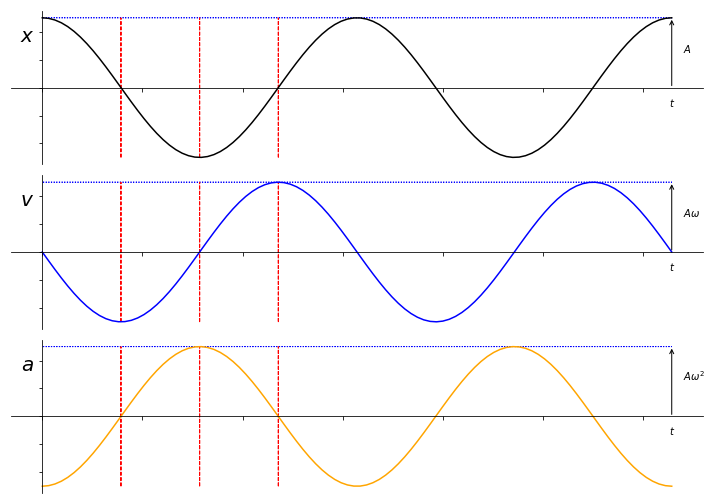
\includegraphics[width=0.7\linewidth]{visualisations/ch1-xvacomp} 

}

\caption{Comparing the changes of position, velocity and acceleration with time for a harmonic oscillator. Note that when $x$ is at zero, $v$ is maximised, while $a$ is at a maximum when $v$ is zero. The relative amplitudes of each of the waves is given.}\label{fig:shm-general-comparison-xva}
\end{figure}

We can now make a few more observations:

\begin{itemize}
\tightlist
\item
  When the displacement \(x\) is at a maximum (\(x_\textrm{max}\)), the velocity \(v\) is zero while the acceleration is at its maximum \textbf{but negative with respect to displacement} (\(a= -a_\textrm{max}\))
\item
  When the displacement \(x\) is zero, the velocity \(v\) is at its maximum value (\(v = \pm v_\textrm{max}\)) and the acceleration is zero.
\item
  The pattern repeats with each period; namely \(x_0\) (displacement at time \(t = 0\)) is equal to the displacement \(x_T\) (displacement after one period of oscillation, \(T\)), and the same for the acceleration and velocity.
\item
  In general, \(x_t = x_{t+T}\); the displacement at time \(t\) is equal to the displacement at the time \(t\) plus one period of oscillation, \(T\).
\end{itemize}

This allows us to compare the displacement, velocity and acceleration at four points in the oscillation (Table \ref{tab:ch1-xva-comparison1}):

\begin{longtable}[]{@{}llll@{}}
\caption{\label{tab:ch1-xva-comparison1} Relating the displacement, velocity and acceleration at different times in the oscillation for a simple harmonic oscillator.}\tabularnewline
\toprule
\begin{minipage}[b]{0.22\columnwidth}\raggedright
Time\strut
\end{minipage} & \begin{minipage}[b]{0.22\columnwidth}\raggedright
Displacement, \(x\)\strut
\end{minipage} & \begin{minipage}[b]{0.22\columnwidth}\raggedright
Velocity, \(v\)\strut
\end{minipage} & \begin{minipage}[b]{0.22\columnwidth}\raggedright
Acceleration, \(a\)\strut
\end{minipage}\tabularnewline
\midrule
\endfirsthead
\toprule
\begin{minipage}[b]{0.22\columnwidth}\raggedright
Time\strut
\end{minipage} & \begin{minipage}[b]{0.22\columnwidth}\raggedright
Displacement, \(x\)\strut
\end{minipage} & \begin{minipage}[b]{0.22\columnwidth}\raggedright
Velocity, \(v\)\strut
\end{minipage} & \begin{minipage}[b]{0.22\columnwidth}\raggedright
Acceleration, \(a\)\strut
\end{minipage}\tabularnewline
\midrule
\endhead
\begin{minipage}[t]{0.22\columnwidth}\raggedright
\(t = 0\)\strut
\end{minipage} & \begin{minipage}[t]{0.22\columnwidth}\raggedright
\(x_0 = A\)\strut
\end{minipage} & \begin{minipage}[t]{0.22\columnwidth}\raggedright
\(v_0 = 0\)\strut
\end{minipage} & \begin{minipage}[t]{0.22\columnwidth}\raggedright
\(a_0 = -a_{\textrm{max}}\)\strut
\end{minipage}\tabularnewline
\begin{minipage}[t]{0.22\columnwidth}\raggedright
\(t = \frac{T}{4}\)\strut
\end{minipage} & \begin{minipage}[t]{0.22\columnwidth}\raggedright
\(x_{\frac{T}{4}} = 0\)\strut
\end{minipage} & \begin{minipage}[t]{0.22\columnwidth}\raggedright
\(v_{\frac{T}{4}} = -v_\textrm{max}\)\strut
\end{minipage} & \begin{minipage}[t]{0.22\columnwidth}\raggedright
\(a_{\frac{T}{4}} = 0\)\strut
\end{minipage}\tabularnewline
\begin{minipage}[t]{0.22\columnwidth}\raggedright
\(t = \frac{T}{2}\)\strut
\end{minipage} & \begin{minipage}[t]{0.22\columnwidth}\raggedright
\(x_{\frac{T}{2}} = -A\)\strut
\end{minipage} & \begin{minipage}[t]{0.22\columnwidth}\raggedright
\(v_{\frac{T}{2}} = 0\)\strut
\end{minipage} & \begin{minipage}[t]{0.22\columnwidth}\raggedright
\(a_{\frac{T}{2}} = a_{\textrm{max}}\)\strut
\end{minipage}\tabularnewline
\begin{minipage}[t]{0.22\columnwidth}\raggedright
\(t = \frac{3T}{4}\)\strut
\end{minipage} & \begin{minipage}[t]{0.22\columnwidth}\raggedright
\(x_{\frac{3T}{4}} = 0\)\strut
\end{minipage} & \begin{minipage}[t]{0.22\columnwidth}\raggedright
\(v_{\frac{3T}{4}} = v_\textrm{max}\)\strut
\end{minipage} & \begin{minipage}[t]{0.22\columnwidth}\raggedright
\(a_{\frac{3T}{4}} = 0\)\strut
\end{minipage}\tabularnewline
\begin{minipage}[t]{0.22\columnwidth}\raggedright
\(t = T\)\strut
\end{minipage} & \begin{minipage}[t]{0.22\columnwidth}\raggedright
\(x_T = x_0 = A\)\strut
\end{minipage} & \begin{minipage}[t]{0.22\columnwidth}\raggedright
\(v_T = v_0 = 0\)\strut
\end{minipage} & \begin{minipage}[t]{0.22\columnwidth}\raggedright
\(a_T = a_0 = -a_{\textrm{max}}\)\strut
\end{minipage}\tabularnewline
\bottomrule
\end{longtable}

\hypertarget{sec:shm-initialconditions}{%
\section{Initial conditions}\label{sec:shm-initialconditions}}

We mentioned in Section \ref{sec:shm-comparing-xva} that the displacement, velocity and acceleration expressions were based on sinusoial functions, and each function had a scaling factor \(A\) (the \textbf{amplitude} of the oscillation) and a \textbf{phase} component \(\delta\). In most problems, we wish to determine the value of these constants. In order to determine these, we establish the initial conditions of the oscillation.

In Figure \ref{fig:shm-general-comparison-xva} we defined our displacement at \(+A\) which set up the rest of the problem. However, we will not always be so fortunate. For a general case, we then need to be more discerning.

We can establish expressions for both the amplitude and the phase component by setting \(t = 0\) in our general expressions (Equation \eqref{eq:ch1-shm-initconditions1}):

\begin{equation}
\begin{array}{rclcrcl}
x &=& A  \cos (\omega t + \delta)       & \rightarrow & x_0 &=& A  \cos (\delta)\\
v &=& -A \omega \sin (\omega t + \delta)& \rightarrow & v_0 &=& -A \omega \sin ( \delta)
\end{array}
\label{eq:ch1-shm-initconditions1}
\end{equation}

We now treat these as simultaneous equations to find \(\delta\) and \(A\) (Equation \eqref{eq:ch1-shm-initconditions2})\footnote{Note that we use the trigonometric identity \(\cos^2 \alpha + \sin^2 \alpha = 1\) to find \(A\)}:

\begin{equation}
\begin{array}{rcl}
\tan \delta = \dfrac{\sin \delta}{\cos \delta} = -\dfrac{v_0}{\omega x_0} & \textrm{and} & A^2 = x_0^2 + \dfrac{v_0^2}{\omega^2}
\end{array}
\label{eq:ch1-shm-initconditions2}
\end{equation}

\hypertarget{sec:shm-freq-angularfreq}{%
\section{Frequency and angular frequency}\label{sec:shm-freq-angularfreq}}

In Section \ref{sec:shm-comparing-xva} we stated that the nature of the oscillation meant that it repeats after every oscillation; mathematically \(x(t) = x(t + T)\); the position \(x\) at time \(t\) is equal to the position at time \((t+T)\).

When we apply this to the velocity, we obtain the following expression:

\begin{equation}
\begin{array}{rcl}
v(t) &=& v(t+T) \\
A \cos (\omega t + \delta) &=& A \cos (\omega (t+T) + \delta) \\
&=& A \cos ([\omega t + \delta] + \omega T)
\end{array}
\end{equation}

Due to the cyclic nature of a cosine function, \(\cos (\alpha) = \cos (\alpha + 2\pi)\), this must therefore mean (Equation \eqref{eq:ch1-definingomega1}):

\begin{equation}
\omega T = 2\pi \hspace{10pt} \textrm{or} \hspace{10pt} \omega = \frac{2\pi}{T}
\label{eq:ch1-definingomega1}
\end{equation}

This gives us a way to think about \(\omega\); its connection to circular motion (the clue is the \(2\pi\)!). It can be thought of as the \textbf{angular frequency}, with units radians s\textsuperscript{-1}, and an oscillation of \(2\pi\) radians corresponds to one period of oscillation.

Additionally, since the frequency of the oscillation \(f\) is the reciprocal of the period of oscillation (\(f = \frac{1}{T}\)), the angular frequency can be rewritten as \(\omega = 2\pi f\), and \(f = \frac{\omega}{2\pi}\).

For the spring system we discussed in Section \ref{sec:ch1-simpleshmexample}, we stated that the angular frequency \(\omega = \sqrt{\frac{k}{m}}\). Therefore we can obtain an expression for the frequency of our oscillator (Equation \eqref{eq:ch1-freq-angfreq1})

\begin{equation}
f = \frac{1}{T} = \frac{1}{2\pi}\sqrt{\frac{k}{m}}
\label{eq:ch1-freq-angfreq1}
\end{equation}

Inspection of this equation reveals the behaviour of our oscillator:

\begin{itemize}
\tightlist
\item
  If we have a stiffer spring (larger \(k\)), we expect the frequency \(f\) to increase,
\item
  If we use an oscillator with larger mass (larger \(m\)), we would expect the frequency (\(f\)) to decrease.
\item
  The frequency (and therefore period) of simple harmonic oscillation is independent of amplitude.\footnote{A caveat to this is for large amplitudes where other factors start to affect the behaviour. But this is then no longer \emph{simple} harmonic motion!}
\end{itemize}

\hypertarget{sec:ch1-shmcircmotion1}{%
\section{SHM and circular motion}\label{sec:ch1-shmcircmotion1}}

We mentioned an ``angular frequency'' for SHM; this would appear to suggest behaviour akin to circular motion. It is therefore worth exploring our descriptions of circular motion.

Imagine a point mass moving in a circle (Figure \ref{fig:ch1-circularmotion1}). For convenience, we imagine this using Cartesian \(x-y\) axes, shown in Figure \ref{fig:ch1-circularmotion1}.

\begin{figure}

{\centering 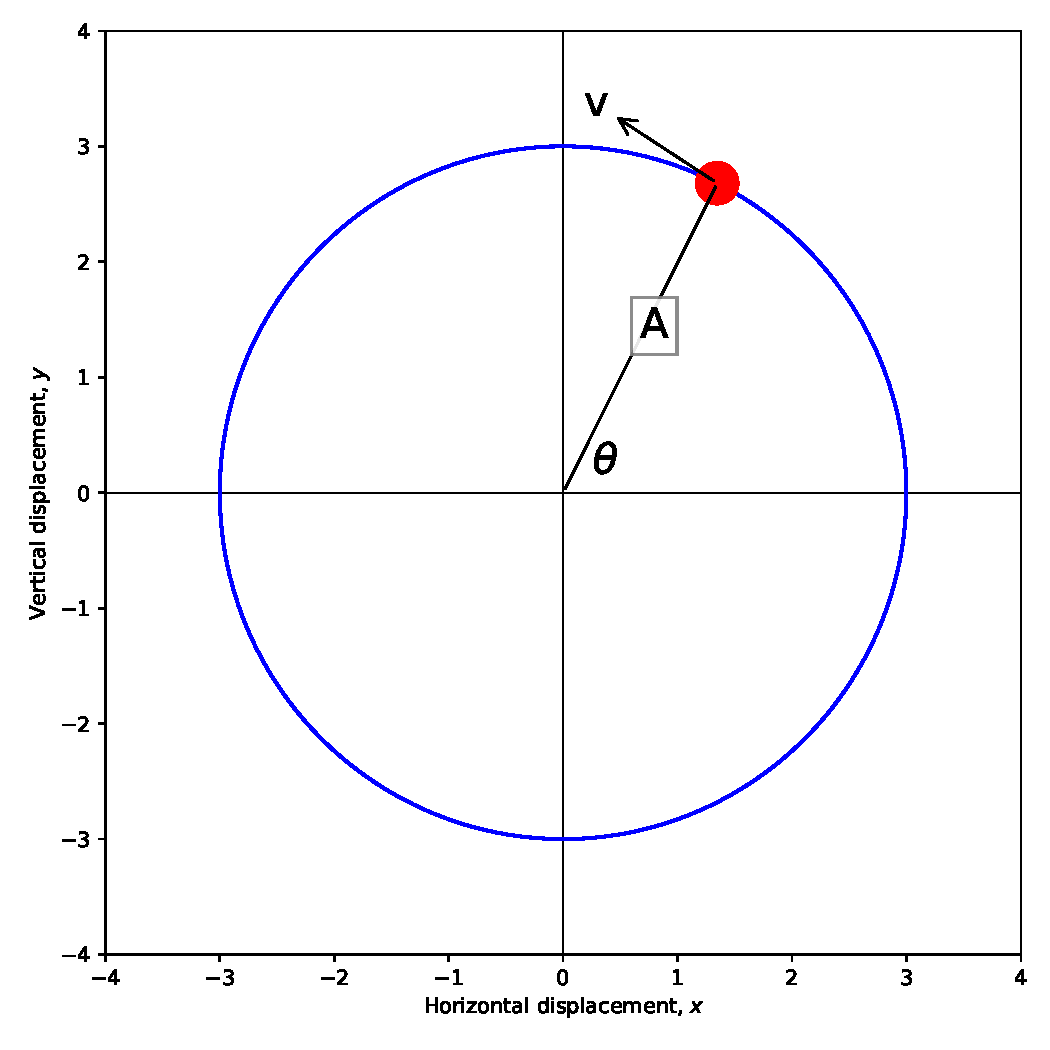
\includegraphics[width=0.7\linewidth]{visualisations/ch1-shmcircular} 

}

\caption{A particle moving in a circle of radius $A$ can be assumed to have an instantaneous linear velocity $v$. The $x$ and $y$ components of the motion are found from trigonometry of the radius $A$ and the angle $θ$.}\label{fig:ch1-circularmotion1}
\end{figure}

The particle of mass \(m\) is moving in a circle of radius \(A\) with instantaneous linear velocity \(v\); the radius makes an angle \(\theta\) with the \(x\)-axis. We now look at how its position maps onto each of the axes:

\begin{itemize}
\tightlist
\item
  The angular velocity of the particle is \(\omega\); found \emph{via} \(\frac{v}{A}\)

  \begin{itemize}
  \tightlist
  \item
    We can then describe \(\theta\) in terms of \(\omega\):
  \item
    \(\theta = \omega t + \delta\) (\(\delta\) is the angle at time \(t=0\))
  \end{itemize}
\item
  The particle's position on the \(x\)-axis is therefore found \emph{via}:

  \begin{itemize}
  \tightlist
  \item
    \(x = A \cos \theta = A \cos (\omega t + \delta)\)
  \item
    This corresponds with the expression for SHM for a particle moving in a linear fashion (Equation \eqref{eq:shm-general-positionx1}).
  \end{itemize}
\end{itemize}

We can also consider how its position maps onto the \(y\)-axis:

\begin{itemize}
\tightlist
\item
  The position on the \(y\)-axis is found \emph{via}:

  \begin{itemize}
  \tightlist
  \item
    \(y = A \sin \theta = A \sin (\omega t + \delta) \equiv A \cos(\omega t + [\delta - \frac{\pi}{2}])\)
  \item
    This once again corresponds with the expression for SHM for a particle moving in a linear fashion.
  \item
    The \(y\)-component of the motion is \(\frac{\pi}{2}\) out of phase wiht the \(x\)-component
  \end{itemize}
\end{itemize}

This illustrates that circular motion is a combination of two perpendicular SHM oscillations of the same frequency and amplitude, but a relative phase of \(\frac{\pi}{2}\).

\hypertarget{sec:ch1-shm-energy1}{%
\section{Energy in SHM}\label{sec:ch1-shm-energy1}}

As with all isolated systems, the total energy \(E\) of the simple harmonic oscillator is constant, however the contributions from potential energy (\(U\)) and KE vary with time.

\begin{equation}
E = KE + U = \textrm{constant}
\end{equation}

Let's go back to the condition for SHM; there is a restoring force proportional to the displacement:

\begin{equation}
F = -kx
\end{equation}

Knowing that the potential energy is the first derivative of the force, we can integrate this force expression (with respect to \(x\)) to get back to the energy statement:\footnote{The constant of integration will evaluate to zero from the starting condition \(U = 0\) at zero displacement.}

\begin{equation}
\begin{array}{rcl}
U &=& \int F \mathrm{d}x \\
& =& \frac{1}{2}kx^2 \hspace{10pt} [+C]
\end{array}
\label{eq:ch1-potentialfromforce1}
\end{equation}

However, we already have an expression for how the displacement, \(x\), varies with time (Equation \eqref{eq:shm-general-positionx1}); let's now substitute this into the result from Equation \eqref{eq:ch1-potentialfromforce1}:

\begin{equation}
U = \frac{1}{2}kA^2 \cos^2 (\omega t + \delta)
\label{eq:ch1-potentialfromforce2}
\end{equation}

We can also generate an expression for the kinetic energy; remember that kinetic energy can be found from \(\frac{1}{2}mv^2\); so we use the expression for \(v\) given in Equation \eqref{eq:shm-general-velocityx1}:

\begin{equation}
\begin{array}{rcl}
KE &=& \frac{1}{2} mv^2 \\
& =& \frac{1}{2} m A^2 \omega^2 \sin^2 (\omega t + \delta)
\end{array}
\label{eq:ch1-potentialfromforce3}
\end{equation}

We can simplify this using Equation \eqref{eq:shm-general-accelerationx1} for a particle on a spring, where \(\omega^2 = \frac{k}{m}\):

\begin{equation}
KE = \frac{1}{2}kA^2 \sin^2 (\omega t + \delta)
\label{eq:ch1-potentialfromforce4}
\end{equation}

Combining the result of Equations \eqref{eq:ch1-potentialfromforce2} and \eqref{eq:ch1-potentialfromforce4} we find the result in Equation \eqref{eq:ch1-potentialfromforce5}:

\begin{equation}
\begin{array}{rcl}
E_\textrm{total} &=& U + KE \\
& =& \frac{1}{2}kA^2 \cos^2 (\omega t + \delta) + \frac{1}{2}kA^2 \sin^2 (\omega t + \delta)\\
& =& \frac{1}{2}kA^2 \left[ \cos^2 (\omega t + \delta) + \sin^2 (\omega t + \delta)\right]\\
&=& \frac{1}{2}kA^2
\end{array}
\label{eq:ch1-potentialfromforce5}
\end{equation}

This result tells us that the total energy in a simple harmonic oscillation is \textbf{proportional to the square of the amplitude}.

\begin{figure}

{\centering 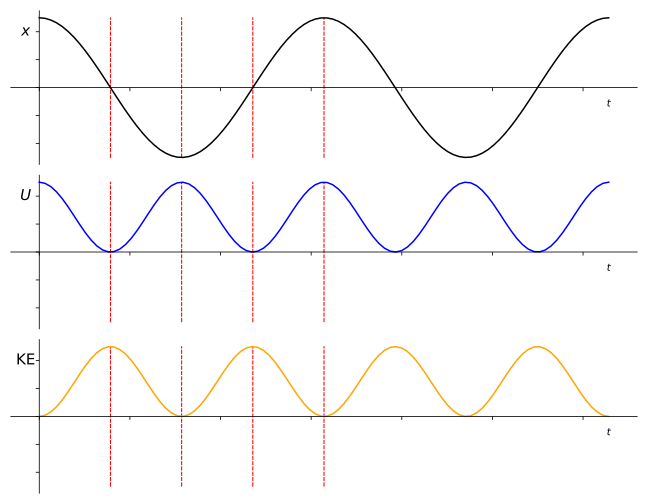
\includegraphics[width=0.7\linewidth]{visualisations/ch1-shmenergy} 

}

\caption{Comparing how the kinetic energy (KE) and potential energy (U) of an harmonic oscillator varies with displacement $x$ about the equilibrium position. }\label{fig:ch1-energyinshm}
\end{figure}

\hypertarget{points-to-bear-in-mind}{%
\subsection{Points to bear in mind}\label{points-to-bear-in-mind}}

\begin{itemize}
\tightlist
\item
  \(U = U_\mathrm{max}\) at \(x = ±x_\mathrm{max}\)
\item
  \(KE = KE_\mathrm{max}\) at \(x = 0\)
\item
  \(U_\mathrm{average} = KE_\mathrm{average} = \frac{1}{2}E_\mathrm{total}\)
\end{itemize}

\hypertarget{sec:shm-real}{%
\chapter{SHM in Real Systems}\label{sec:shm-real}}

\emph{Textbook link: Tipler and Mosca: Ch 14.2 to 14.4}

\hypertarget{general-motion-near-equilibrium}{%
\section{General motion near equilibrium}\label{general-motion-near-equilibrium}}

A way of thinking about SHM is that it is a point mass oscillating within a potential energy field. As with any potential energy field, the force on this particle is given by the gradient of the potential energy and is directed down the potential energy slope. Mathematically, for a potential energy field, the force may be found as follows (Equation \eqref{eq:ch2-forceenergyderiv1}):

\begin{equation}
F = - \frac{\mathrm{d}U}{\mathrm{d}r}
\label{eq:ch2-forceenergyderiv1}
\end{equation}

In a one-dimensional system, this is expressed as follows (Equation \eqref{eq:ch2-forceenergyderiv2}):

\begin{equation}
F_x = - \frac{\mathrm{d}U}{\mathrm{d}x}
\label{eq:ch2-forceenergyderiv2}
\end{equation}

As mentioned in Section \ref{sec:ch1-simpleshmexample}, under SHM the force is proportional to the displacement from the equilibrium position and in the opposite direction; i.e.:

\begin{equation}
F_x = -kx
\label{eq:ch2-hookeslaw1}
\end{equation}

Applying the principle from Equation \eqref{eq:ch2-forceenergyderiv1} we can therefore integrate this experession with respect to \(x\) to obtain the expression for our potential energy. We covered this in Section \ref{sec:ch1-shm-energy1}, and we found the result (Equation \eqref{eq:ch2-potentialfromforce1}; remember that, due to initial conditions, the constant of integration reduces to zero).

\begin{equation}
U  = \frac{1}{2}kx^2 
\label{eq:ch2-potentialfromforce1}
\end{equation}

Simple inspection and recall of our mathematics knowledge tells us that this simple equation represents a parabola. This gives us a series of useful points to bear in mind:

\begin{itemize}
\tightlist
\item
  A parabolic potential energy function implies SHM and \emph{vice versa};
\item
  For small amplitudes of oscillation, many potential energy functions may be \emph{approximated} by a parabola (\emph{e.g.} a pendulum, vibrating molecules)
\item
  A system undergoing SHM is called a \textbf{harmonic oscillator}.
\end{itemize}

The simplicity of the \textbf{simple harmonic oscillator} model is what makes it such a generally useful system to consider.

\hypertarget{sec:ch2-diatomicmolecule}{%
\section{Example: a diatomic molecule}\label{sec:ch2-diatomicmolecule}}

A diatomic molecule is a useful system to consider as an example because it can be very usefully approximated to a harmonic oscillator. The potential energy curve for a vibrating diatomic molecule (in this case the H\_2\_ hydrogen molecule) is shown in Figure \ref{fig:ch2-diatomicmolecule1}.

\begin{figure}

{\centering 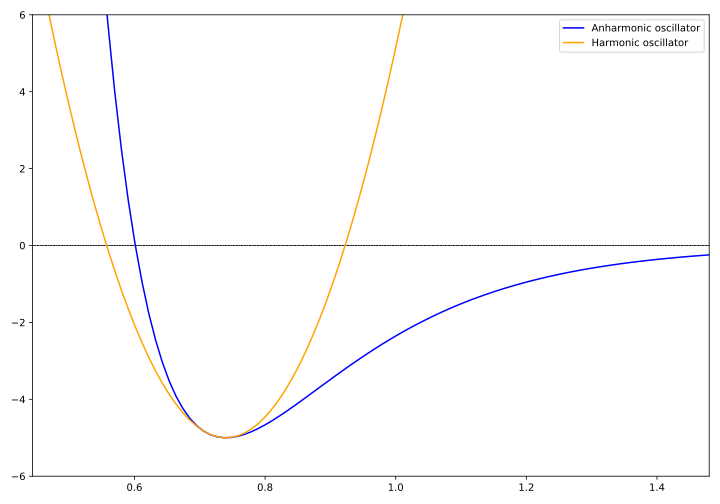
\includegraphics[width=0.7\linewidth]{visualisations/ch2-diatomicexamp} 

}

\caption{Comparing the Morse potential of the anharmonic oscillator with the harmonic approximation. Near equilibrium, the harmonic oscillator model approximates diatomic behaviour, however this rapidly deviates from reality. }\label{fig:ch2-diatomicmolecule1}
\end{figure}

The potential of a vibrating diatomic is known as the Morse potential; the form of this is outwith this discussion, however it is useful to think that, for small displacements around the equilibrium separation the potential energy curve approximates a parabola. We can therefore re-draw our potential energy curve as such, and show this in Figure \ref{fig:ch2-diatomicmolecule2}.\footnote{Simplistically, the deviation is due to nuclear repulsion at high compression, while at large extension the bond eventually breaks - the ``zero potential'' point.}

\begin{figure}

{\centering 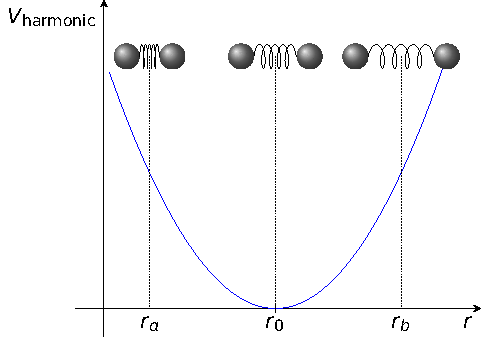
\includegraphics[width=0.7\linewidth]{visualisations//latex/ch2-diatomicmolecule2} 

}

\caption{The parabolic approximation of a diatomic molecule, showing the potential varying with compression or extension from equilibrium separation, $r_0$. }\label{fig:ch2-diatomicmolecule2}
\end{figure}

The equation of the parabola shown in \ref{fig:ch2-diatomicmolecule2} takes the following form:

\begin{equation}
U(r) = A + B(r - r_0)^2
\label{eq:ch2-diatomicmolecule1}
\end{equation}

\ldots where \(A\) and \(B\) are constants relating to the molecular system under consideration, and \(r_0\) is the equilibrium bond length.

The force on the bond can then be found from the first derivative of the bond potential described in Equation \eqref{eq:ch2-diatomicmolecule1}:

\begin{equation}
\begin{array}{rcl}
F_r &=& - \dfrac{\mathrm{d}U}{\mathrm{d}r} \\
\\
&=& -2B(r-r_0)\\
\end{array}
\label{eq:ch2-diatomicmolecule2}
\end{equation}

Since the term \((r-r_0)\) is the displacement from the equilibrium position, we see that the force, \(F_r\) is a \textbf{restoring force} and is proportional to the displacement (and in the opposite direction!), telling us that the motion is SHM. In this example however, the parabolic approximation fails at larger amplitudes.

\hypertarget{sec:ch2-massverticalspring}{%
\section{Example: Mass on a vertical spring}\label{sec:ch2-massverticalspring}}

In Section \ref{sec:ch1-simpleshmexample} we considered a mass on a horizontal spring; there was only a single force acting on the mass (the force from the spring), however we are now considering a vertical spring and must consider the effects of gravity (Figure \ref{fig:ch2-massverticalspring1}).

\begin{figure}

{\centering 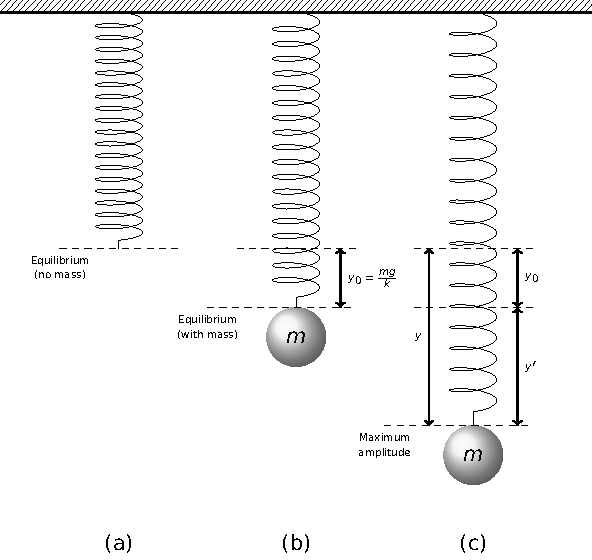
\includegraphics[width=0.7\linewidth]{visualisations/LaTeX/ch2-blocksonvertspring1} 

}

\caption{A particle oscillating on a vertical spring.  There are two equilibrium positions corresponding to the equilibrium position of the unladen spring (a) and the equilibrium position of the mass loaded on spring (b), where the weight of the load is balanced by the force from the extended spring.}\label{fig:ch2-massverticalspring1}
\end{figure}

In this case we need to work through a slightly different process to find the equation of motion, chiefly because the equilibrium displacement of the mass (\(y_0\)) is different from the equilibrium position of the spring.

The equilibrium position of the mass \(y_0\) is lower than the equilibrium extension of the spring (gravity on the mass causes the spring to stretch). This is found by relating the force from the spring and the force of gravity acting on the mass (Equation \eqref{eq:ch2-massverticalspring1}):

\begin{equation}
\begin{array}{rcl}
\mathrm{Force~due~to~spring~extension} &=& \mathrm{Gravity~acting~on~mass}\\
k y_0 &=& mg\\
y_0 &=& \dfrac{mg}{k}\\
\end{array}
\label{eq:ch2-massverticalspring1}
\end{equation}

We now apply Newton's Second Law to obtain an expression for the acceleration on the mass due to the forces acting on it (the spring force and gravity).

\begin{equation}
\begin{array}{rcl}
m\ddot{y}&=&  \textrm{spring force} + \textrm{gravity} \\
m\dfrac{\mathrm{d}^2 y}{\mathrm{d} t^2} &=& -ky + mg\\
\end{array}
\label{eq:ch2-massverticalspring2}
\end{equation}

In this expression, \(y\) is the total extension of the spring (the extension to the mass equilibrium point, \(y_0\) plus the displacement from this point, \(y^\prime\)).

We now substitute a variable; since \(y = y_0 + y^\prime\), we substitute \(y\) for \(y^\prime\):

\begin{itemize}
\tightlist
\item
  \(y = y_0 + y^\prime\)
\item
  \(y^\prime = y - y_0\)
\end{itemize}

Since \(y_0\) is a constant:

\begin{equation}
\dfrac{\mathrm{d} y^\prime}{\mathrm{d} t} = \dfrac{\mathrm{d} y}{\mathrm{d} t} \hspace{10pt} \textrm{and} \hspace{10pt} \dfrac{\mathrm{d}^2 y^\prime}{\mathrm{d} t^2} = \dfrac{\mathrm{d}^2 y}{\mathrm{d} t^2}
\end{equation}

Replacing \(y\) for \((y_0 + y^\prime)\) in Equation \eqref{eq:ch2-massverticalspring2}, we obtain Equation \eqref{eq:ch2-massverticalspring3}:

\begin{equation}
m\dfrac{\mathrm{d}^2 y^\prime}{\mathrm{d} t^2} = -k(y_0 + y^\prime) + mg
\label{eq:ch2-massverticalspring3}
\end{equation}

Since \(ky_0 = mg\) (Equation \eqref{eq:ch2-massverticalspring1}), we can therefore eliminate these terms from Equation \eqref{eq:ch2-massverticalspring3}, and rewrite as Equation \eqref{eq:ch2-massverticalspring4}:

\begin{equation}
m\dfrac{\mathrm{d}^2 y^\prime}{\mathrm{d} t^2} = -k y^\prime
\label{eq:ch2-massverticalspring4}
\end{equation}

This means that, in reference to Figure \ref{fig:ch2-massverticalspring1}, we still have SHM centered on the equilibrium position of the mass. This may seem like a self-evident result, however it is useful to recognise the role of gravity; its effect is to shift the equilibrium position of the oscillation from \(y = 0\) (the equilibrium position of the spring) to \(y = y_0\) (\(y^\prime = 0\)).

Let's now consider the energy in this system. The system already contains some elastic energy as the spring is already stretched to \(y_0\) by the gravity acting on the mass:

\begin{equation}
\textrm{elastic potential energy} = \frac{1}{2}ky^2 - \frac{1}{2}ky_0^2
\end{equation}

The gravitational potential energy (relative to the starting position \(y_0\)) is given by:

\begin{equation}
\textrm{gravitational potential energy} = mg(y-y_0)
\end{equation}

The total potential energy is therefore given by Equation \eqref{eq:ch2-massverticalspring5}:

\begin{equation}
U = \frac{1}{2}ky^2 - \frac{1}{2}ky_0^2 - mg(y-y_0)
\label{eq:ch2-massverticalspring5}
\end{equation}

We can then show that the total potential energy expression in Equation \eqref{eq:ch2-massverticalspring5} can be simplified to that shown in Equation \eqref{eq:ch2-massverticalspring6}:

\begin{equation}
U = \frac{1}{2} ky^{\prime 2}
\label{eq:ch2-massverticalspring6}
\end{equation}

\textbf{You should ensure you understand how this simplification is done}; this is left as an exercise.

Overall, the expression for the total potential energy shown in Equation \eqref{eq:ch2-massverticalspring6} will still yield a parabola and as such the oscillation is still a simple harmonic oscillation as before.

\hypertarget{sec:ch2-simplependulum}{%
\section{The Simple Pendulum}\label{sec:ch2-simplependulum}}

A pendulum is a mechanically simple oscillating system; its oscillation can be considered SHM for small displacements. A simple pendulum is shown in Figure \ref{fig:ch2-simplependulum1}, and it is worth quickly revisiting this example as we will extend this in our futher examples.

\begin{figure}

{\centering 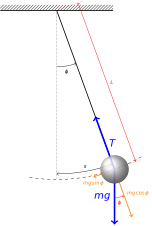
\includegraphics[width=0.7\linewidth]{visualisations/LaTeX/ch2-simplependulum1} 

}

\caption{A simple pendulum, consisting of a mass $m$ swinging on a string of length $L$. At angle $\phi$, the weight of the mass $mg$ can be resolved into components to determine the mechanics of the system.}\label{fig:ch2-simplependulum1}
\end{figure}

For small dispalcements (small \(\phi\)), the equation of motion can be considered as in Equation \eqref{eq:ch2-simplependulum1}:

\begin{equation}
\frac{\mathrm{d}^2 \phi}{\mathrm{d} t^2} = -\frac{g}{L}\sin \theta \approx -\frac{g \phi}{L} \textrm{for small} \phi
\label{eq:ch2-simplependulum1}
\end{equation}

This is SHM, with angular frequency \(\omega\) and period \(T\) found as in Equation \eqref{eq:ch2-simplependulum2}:

\begin{equation}
\omega^2 = \frac{g}{L} \hspace{15pt} and \hspace{15pt} T = 2\pi \sqrt{\frac{L}{g}}
\label{eq:ch2-simplependulum2}
\end{equation}

The solution for the equation of motion of this system then becomes (Equation \eqref{eq:ch2-simplependulum3}):

\begin{equation}
\phi = \phi_0 \cos (\omega t + \delta)
\label{eq:ch2-simplependulum3}
\end{equation}

\ldots where \(\phi_0\) is the amplitude of the system and \(\delta\) is the phase constant. Notice that, for the pendulum we express the amplitude in terms of the angle of the string rather than an absolute distance (shown as \(s\) in Figure \ref{fig:ch2-simplependulum1}).

\hypertarget{sec:ch2-physicalpendulum}{%
\section{The Physical Pendulum}\label{sec:ch2-physicalpendulum}}

Many oscillating systems demonstrate rotational oscillations under gravity akin to the simple pendulum. In this case, the system rotates around a pivot, \(P\), and this can then be considered as a pendulum with the centre of mass acting as the `bob'. An example of a general system is shown in Figure \ref{fig:ch2-physicalpendulum1}.

\begin{figure}

{\centering 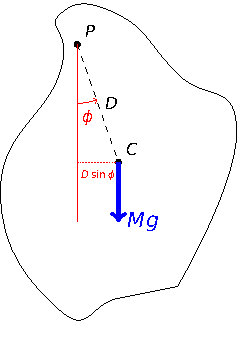
\includegraphics[width=0.4\linewidth]{visualisations/LaTeX/ch2-physicalpendulum1} 

}

\caption{A physical pendulum, consisting of a physical object of mass $M$ swinging on a pivot through point $P$ of length $L$. At angle $\phi$, the weight of the mass $Mg$ can again be resolved into components to determine the mechanics of the system.}\label{fig:ch2-physicalpendulum1}
\end{figure}

Now, as a restoring force, we consider the \textbf{torque} of the centre of mass around the pivot. Remember that the torque is defined as the product of the force and the \textbf{perpendicular distance of the force's line of action from the pivot}. If using vectors, this is considered as the \textbf{cross product} of the force vector \(\mathbf{F}\) with the position vector of the centre of mass from the pivot, \(\mathbf{D}\) (Equation \eqref{eq:ch2-physicalpendulum1}):

\begin{equation}
\begin{array}{rcl}
\textrm{Torque about pivot $P$} &=& \mathbf{F} \times \mathbf{D} \\
&=& \mathbf{\hat{n}}~ |F| |D| \sin \phi \\
&=& \mathbf{\hat{n}}~ mg D \sin \phi = \tau \mathbf{\hat{n}} 
\end{array}
\label{eq:ch2-physicalpendulum1}
\end{equation}

In this case, the unit vector \(\mathbf{\hat{n}}\) is perpendicular to the plane of rotation and is included for completeness' sake. What we are interested in is the magnitude of this torque vector, \(\tau\).

Recall from rotational motion that the angular acceleration \(\alpha\) and the torque \(\tau\) are connected via the moment of inertia \(I\) (Equation \eqref{eq:ch2-physicalpendulum2}):\footnote{Note that the appearance of the negative sign indicates that the torque force is opposite to the direction of increasing \(\phi\)}

\begin{equation}
\begin{array}{rcl}
I \dfrac{\mathrm{d}^2 \phi}{\mathrm{d} t^2}  &=& I\alpha =\tau \\
&=& -mgD \sin \phi
\end{array}
\label{eq:ch2-physicalpendulum2}
\end{equation}

We now approximate this for small \(\phi\):

\begin{equation}
\frac{\mathrm{d}^2 \phi}{\mathrm{d} t^2} = -\frac{mgD\phi}{I} = -\omega^2 \phi
\end{equation}

This allows us to identify expressions again for the angular frequency, \(\omega\), and the period \(T\) (Equation \eqref{eq:ch2-physicalpendulum3}):

\begin{equation}
\omega^2 = \frac{mgD}{I} \hspace{15pt} and \hspace{15pt} T = 2\pi \sqrt{\frac{I}{mgD}}
\label{eq:ch2-physicalpendulum3}
\end{equation}

We can compare this result with that for the simple pendulum shown in Equation \eqref{eq:ch2-simplependulum2}; if we remember that the moment of inertia \(I\) is defined as \(I = mD^2\), we can substitute this into Equation \eqref{eq:ch2-physicalpendulum3} and see that this is a general case for any rotating body:

\begin{equation}
T_\textrm{simple pendulum} = 2\pi \sqrt{\frac{I_\textrm{simple pendulum}}{mgD}} = 2\pi \sqrt{\frac{mD^2}{mgD}} = 2\pi \sqrt{\frac{D}{g}}
\end{equation}

\ldots giving us our expected result (where the general term \(D\) can be replaced for the length of the simple pendulum, \(L\)).

\hypertarget{sec:ch3-complexnumbers}{%
\chapter{Complex Numbers}\label{sec:ch3-complexnumbers}}

\emph{Textbook link: Jordan and Smith, Ch. 6}

As we move on with our descriptions of oscillations and, in particular, wave behaviour, the mathematics can become increasingly involved. We can greatly simplify the mathematics by using \textbf{complex numbers} in our derivations. For now, it is useful to quickly revisit the complex number concept.

While the idea of a ``complex number'' sounds \ldots{} \emph{complex}, the use of these numbers becomes straightforward as we apply our familiar mathematical techniques. In the context of mathematics, the term \textbf{complex} simply means `more than one part'; therefore, a \textbf{complex number} is a number with more than one part. It is this two-component nature of a complex number which makes them so useful in many aspects of Physics, and particularly when describing wave behaviour.

\hypertarget{sec:ch3-complexoverview}{%
\section{Overview of complex numbers}\label{sec:ch3-complexoverview}}

The general form of a complex number \(z\) is shown in Equation \eqref{eq:ch3-complexnumber1}:

\begin{equation}
z = a + \mathrm{i}b
\label{eq:ch3-complexnumber1}
\end{equation}

The symbol \(z\) is a general term for a complex number, and has two components, a ``real'' component \(a\) and an ``imaginary'' component, \(b\). The imaginary number, \(\mathrm{i}\), is defined using the process shown in Equation \eqref{eq:ch3-complexnumber2}:

\begin{equation}
\begin{array}{rcl}
x^2 &=& -1 \\
x &=& \pm \mathrm{i}\\
i^2 &=& -1
\end{array}
\label{eq:ch3-complexnumber2}
\end{equation}

The terms `real' and `imaginary' are nothing more than labels. Neither is any more or less ``realistic'' than the other nor is it any less valid. Some may claim that the number \(\mathrm{i}\) is a `pretend' number; however were this to be true, it would not be as useful as it is!\footnote{Remember that negative numbers were once seen as `pretend numbers', as you could not have negative eight apples. They have since become indispensable in many applications, not least financial transactions!}.

The next useful concept to recall is the \textbf{complex conjugate}, \(z^*\). This is defined as in Equation \eqref{eq:ch3-complexnumber3}:

\begin{equation}
\begin{array}{rcl}
z &=& a + \mathrm{i}b \\
z* &=& a - \mathrm{i}b \\
zz^* &=& a^2 + b^2
\end{array}
\label{eq:ch3-complexnumber3}
\end{equation}

In general, for any complex number of the form \(z = a \pm \mathrm{i}b\), there exists its complex conjugate, \(z^* = a \mp \mathrm{i}b\) such that \(zz^*\) is a wholly real number and equal to \(a^2 + b^2\).

The complex conjugate is particularly useful when finding fractions of complex numbers as it is used to make the denominator of the fraction wholly ``real''.

\hypertarget{sec:ch3-complexusefulresults}{%
\section{Useful results for complex numbers}\label{sec:ch3-complexusefulresults}}

There are a number of useful results worth remembering when handling complex numbers, and these are listed here.

For a pair of complex numbers, \(z_1\) and \(z_2\):

\begin{equation}
\begin{array}{rcl}
z_1 &=& a_1 + \mathrm{i}b_1 \\
z_2 &=& a_2 + \mathrm{i}b_2 
\end{array}
\label{eq:ch3-complexnumber4}
\end{equation}

\ldots we can establish the following principles:

\begin{itemize}
\tightlist
\item
  Equality:
\end{itemize}

\begin{equation}
\textrm{If} \hspace{15pt} a_1 = a_2 \hspace{15pt} \textbf{and} \hspace{15pt} b_1 = b_2  \hspace{15pt} \textrm{then}  \hspace{15pt} z_1 = z_2
\end{equation}

\begin{itemize}
\tightlist
\item
  Addition and subtraction:
\end{itemize}

\begin{equation}
\begin{array}{rcl}
z_1 + z_2 &=& (a_1 + a_2) + \mathrm{i}(b_1 + b_2) \\
z_1 - z_2 &=& (a_1 - a_2) + \mathrm{i}(b_1 - b_2) \\
\end{array}
\end{equation}

\begin{itemize}
\tightlist
\item
  Products:
\end{itemize}

\begin{equation}
\begin{array}{rcl}
z_1 \times  z_2 &=& (a_1 + \mathrm{i}b_1) (a_2 + \mathrm{i}b_2) \\
 &=& (a_1 a_2 - b_1 b_2) + \mathrm{i}(a_1 b_2 + a_2 b_1) \\
\end{array}
\end{equation}

\begin{itemize}
\tightlist
\item
  Reciprocal:
\end{itemize}

\begin{equation}
\frac{1}{z} = \frac{z^* }{z z^* } = \frac{a - \mathrm{i}b }{a^2 + b^2 }
\end{equation}

\begin{itemize}
\tightlist
\item
  Division:
\end{itemize}

\begin{equation}
\frac{z_1}{z_2} = \frac{z_1 z_2^* }{z_2 z_2^* } = \frac{(a_1 a_2 + b_1 b_2) - \mathrm{i}(a_1 b_2 - a_2 b_1)}{a_2^2 + b_2^2 }
\end{equation}

Other useful principles which involve the complex conjugate are listed in Equation \eqref{eq:ch3-complexnumber5} below:

\begin{equation}
\begin{array}{rcl}
(z_1 + z_2)^* &=& z_1^* + z_2^*\\
(z_1  z_2)^* &=& z_1^* + z_2^* \\
\left( \dfrac{z_1}{z_2} \right)^* &=& \dfrac{z_1^* }{z_2^* } \\
a = \mathrm{Re}(z) &=& \dfrac{1}{2}(z + z^* ) \\
b = \mathrm{Im}(z) &=& \dfrac{1}{2}(z - z^* ) 
\end{array}
\label{eq:ch3-complexnumber5}
\end{equation}

\hypertarget{sec:ch3-arganddiagram}{%
\section{The Argand Diagram}\label{sec:ch3-arganddiagram}}

Since a complex number consists of two independent components, we have another way to describe these numbers. Complex numbers can be plotted on a graph, with the `\textbf{real}' component plotted on one axis (the \(x\)-axis) and the `\textbf{imaginary}' component plotted on the other axis (the \(y\)-axis). This is the basis of the Argand diagram (Figure \ref{fig:ch3-argand1}).

\begin{figure}

{\centering 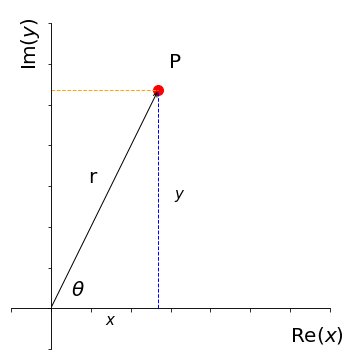
\includegraphics[width=0.7\linewidth]{visualisations/ch3-complexnumbers1} 

}

\caption{A typical Argand diagram, showing the Real ('Re') axis and the Imaginary ('Im') axis. The point $P$ can be defined in '$x,y$' terms (the 'complex number'), or can be defined as polar '$r,\theta$' terms (termed 'modulus' and 'argument')}\label{fig:ch3-argand1}
\end{figure}

This allows us to define a complex number in terms of a \textbf{modulus} (radial distance from the origin) and an \textbf{argument} (angle from the `real' axis). Useful properties of the modulus are listed in Equation \eqref{eq:ch3-complexnumber6}:

\begin{equation}
\begin{array}{rcl}
|z^* | &=& |z| \\
zz^* &=& |z^2| \\
 |z_1 z_2| &=& |z_1 | |z_2| \\
|\dfrac{z_1}{z_2}| &=& \dfrac{|z_1|}{|z_2|} \\
\\
|z_1 + z_2| &\neq& |z_1 | + |z_2|
\end{array}
\label{eq:ch3-complexnumber6}
\end{equation}

The Argand diagram is a representation of the \textbf{complex plane}, through which it becomes possible to visualise properties of complex numbers. One example of this is the addition of complex numbers; these can be considered to behave as vectors (Figure \ref{fig:ch3-argandcomplexaddition1})

\begin{figure}

{\centering 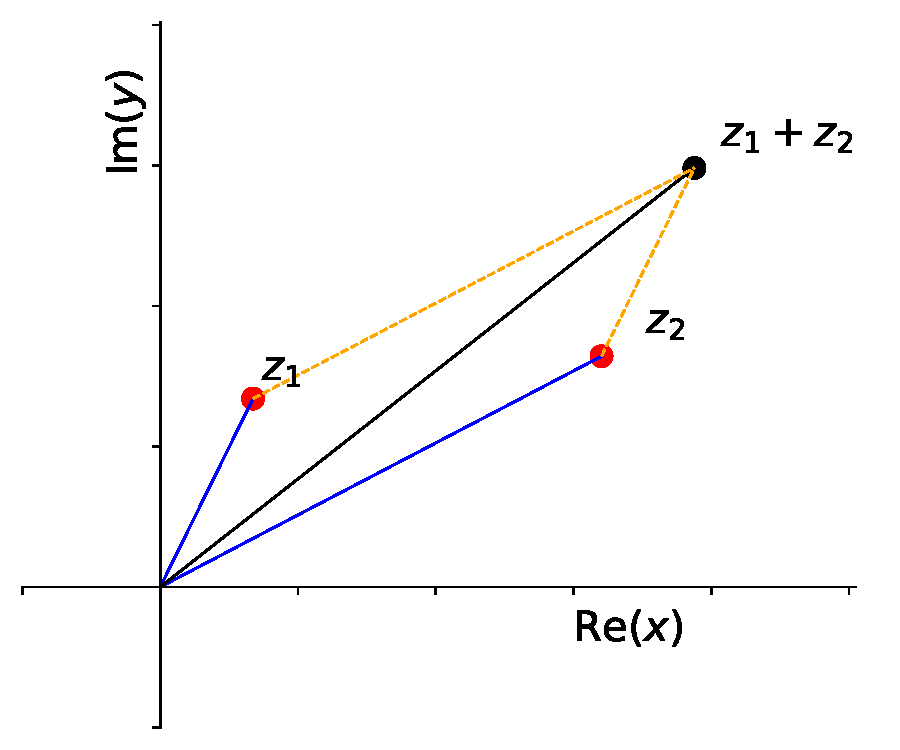
\includegraphics[width=0.7\linewidth]{visualisations/ch3-complexnumbers2} 

}

\caption{Addition of complex numbers $z_1$ and $z_2$ can be shown grapically on an Argand diagram; the separate consideration of the 'real' and 'imaginary' components is analogous to the separate consideration of vector components.}\label{fig:ch3-argandcomplexaddition1}
\end{figure}

\hypertarget{sec:ch3-polarcomplexnumbers}{%
\section{Polar representation of complex numbers}\label{sec:ch3-polarcomplexnumbers}}

As well as the \textbf{cartesian interpretation} of the Argand diagram, we can also consider a \textbf{polar representation} of a complex number; where instead of ``real'' and ``imaginary'' components acting as \((x,y)\) coordinates, we define the position of the complex number on the complex plane as a radius and an angle, \(\theta\). We have already illustrated this in Figure \ref{fig:ch3-argand1}

In this representation, the complex number can be expressed a different way:

\begin{equation}
\begin{array}{rcl}
& z = a + \mathrm{i}b & \\
& r = |z| = \sqrt{a^2 + b^2} & \\
a = r\cos \theta & b = r \sin \theta & \theta = \mathrm{arg} (z) = \arctan \left( \dfrac{b}{a} \right) \\
& z = r \cos \theta + \mathrm{i}|z| \sin \theta &
\end{array}
\end{equation}

Normally, \(\theta\) will lie in the range such that \(-\pi < \theta \leq \pi\), meaning that our complex number representation is now shown in Equation \eqref{eq:ch3-complexnumber7}:

\begin{equation}
\begin{array}{c}
z = a + \mathrm{i}b = r \cos \theta + \mathrm{i} r \sin \theta \\
z = r \left( \cos \theta + \mathrm{i} \sin \theta \right)
\end{array}
\label{eq:ch3-complexnumber7}
\end{equation}

\hypertarget{sec:ch3-exponentialrepresentationcomplex}{%
\section{Exponential representation of complex numbers}\label{sec:ch3-exponentialrepresentationcomplex}}

The exponential representation of a complex number takes the general form of \(z = Ae^{\mathrm{i}\theta}\). This is based on series expansions of \(\cos \theta\) and \(\mathrm{i}\sin \theta\), which shows \emph{De Moivre's theorem}. Key results from this are shown in Equation \eqref{eq:ch3-demoivre1}:

\begin{equation}
\begin{array}{rcl}
\mathrm{e}^{\mathrm{i}\theta} &= &\cos \theta + \mathrm{i}\sin \theta\\
\left( \mathrm{e}^{\mathrm{i}\theta} \right)^n &=& \left( \cos \theta + \mathrm{i}\sin \theta \right)^n = \mathrm{e}^{\mathrm{i}n\theta} \\
\left( \cos \theta + \mathrm{i}\sin \theta \right)^n &=&  \cos n\theta + \mathrm{i}\sin n \theta
\end{array}
\label{eq:ch3-demoivre1}
\end{equation}

This means that we obtain the following representations for complex numbers:

\begin{equation}
\begin{array}{c}
z = r \left( \cos \theta + \mathrm{i}\sin \theta \right) = r\mathrm{e}^{\mathrm{i}\theta}\\
z^* = r \left( \cos \theta - \mathrm{i}\sin \theta \right) = r\mathrm{e}^{-\mathrm{i}\theta}\\
\textrm{where:} \hspace{15pt} r = |z| \hspace{20pt} \theta = \textrm{arg}(z)
\end{array}
\end{equation}

Combining these with Equation \eqref{eq:ch3-complexnumber5} we also note the following useful results (Equation \eqref{eq:ch3-complexnumber8})

\begin{equation}
\begin{array}{rcl}
\cos \theta &=& \frac{1}{2} \left( \mathrm{e}^{\mathrm{i}\theta} + \mathrm{e}^{-\mathrm{i}\theta} \right)\\
\sin \theta &=& \frac{1}{2\mathrm{i}} \left( \mathrm{e}^{\mathrm{i}\theta} - \mathrm{e}^{-\mathrm{i}\theta} \right)\\
\end{array}
\label{eq:ch3-complexnumber8}
\end{equation}

\hypertarget{sec:ch3-complexreposcillation}{%
\section{Complex representation of oscillations}\label{sec:ch3-complexreposcillation}}

Having quickly readdressed our understanding of complex numbers, we now turn our attention to the application of these in the context of oscillations and waves.

Consider the general equation of SHM (Equation \eqref{eq:ch3-complexoscill1}, derived from Equation \eqref{eq:shm-general-accelerationx2})

\begin{equation}
\frac{\mathrm{d}^2 u}{\mathrm{d} t^2 } + \omega^2 u = 0
\label{eq:ch3-complexoscill1}
\end{equation}

As has been previously discussed, sinusoidal functions can form the basis of solutions to this differential equation; so both \(\cos \omega t\) and \(\sin \omega t\) are solutions to this equation. Therefore, any linear combination of these solutions will also be a solution, \emph{i.e.} the linear combination shown here:

\begin{equation}
u = c_1 \cos \omega t + c_2 \sin \omega t
\end{equation}

\ldots{} will also satisfy Equation \eqref{eq:ch3-complexoscill1}. This can be extended using De Moivre's theorem (Equation \eqref{eq:ch3-demoivre1}) allowing an exponential representation of an oscillation as shown in Equation \eqref{eq:ch3-demoivreoscillation1}:

\begin{equation}
u = A (\cos \omega t + \mathrm{i} \sin \omega t) \equiv A \mathrm{e}^{\mathrm{i}\omega t}
\label{eq:ch3-demoivreoscillation1}
\end{equation}

Therefore the solution \(u = A\mathrm{e}^{\mathrm{i}\omega t}\) represents an oscillation with amplitude \(A\) and frequency \(\omega\)

\hypertarget{take-home-points}{%
\section{Take-home points}\label{take-home-points}}

\begin{itemize}
\tightlist
\item
  We can \textbf{always} represent an oscillation using a complex exponential function
\item
  To obtain the actual physical displacement of the system we simply examine either the real or the imaginary part of the solution:
\end{itemize}

\begin{equation}
\begin{array}{lrcl}
\textsf{Either:} & \textrm{displacement} &=& \mathrm{Re}(u) = A \cos \omega t \\
\textsf{or:} & \textrm{displacement} &=& \mathrm{Im}(u) = A \sin \omega t
\end{array}
\end{equation}

The main advantage of working with complex exponentials is that they are considerably easier to manipulate than the trigonometric functions sine and cosine. In general it is far easier to use this exponential notation when multiplying oscillations (such as you will explore in electrical circuits later). However, when adding oscillations or waves you may find it easier using a trigonometric identity.

You should be comfortable using either approach to represent an oscillation.

\hypertarget{sec:ch4-dampedoscillations}{%
\chapter{Damped oscillations}\label{sec:ch4-dampedoscillations}}

\emph{Textbook link}

The oscillations we have looked at so far make the assumption that the oscillation will continue indefinitely and that no energy is gained or lost by the system. Such perpetually oscillating systems are extremely unusual, and almost every oscillation you encounter in the real world will lose energy to its surroundings, either requiring constant input of energy to maintain the oscillation or it will eventually dissipate all of its energy and the oscillation will stop. The energy is dissipated through a process known as `damping'.

\begin{figure}

{\centering 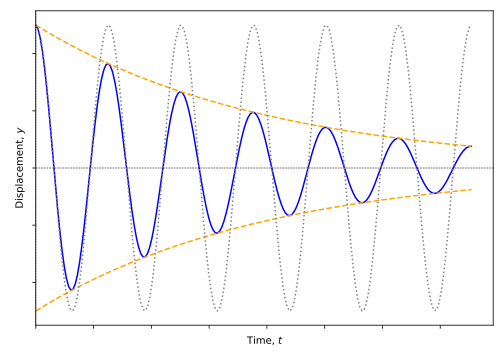
\includegraphics[width=0.7\linewidth]{visualisations/ch4-dampedoscill1} 

}

\caption{The amplitude of a damped oscillation decays exponentially with time.  The observed position of the oscillation is shown in blue, while the maximum possible amplitude (related to energy stored in the system) is illustrated by the orange dotted line.  The undamped oscillation is shown in grey for comparison.}\label{fig:ch4-dampedoscillation1}
\end{figure}

The change in amplitude of a damped oscillation is illustrated in Figure \ref{fig:ch4-dampedoscillation1}. Both amplitude and energy decrease by a \textbf{constant percentage} in each cycle; this is an \textbf{exponential decrease}.

\hypertarget{sec:ch4-generalcasedamping}{%
\section{The general case of damping}\label{sec:ch4-generalcasedamping}}

For a simply damped system, the damping force is proportional to the velocity of the oscillating mass and \textbf{opposes} the direction of motion (Equation \eqref{eq:ch4-velocitydamp1}):

\begin{equation}
F = -bv \equiv -b \frac{\mathrm{d}x}{\mathrm{d} t}
\label{eq:ch4-velocitydamp1}
\end{equation}

This expression for the damping force can then be included with the equation for the force from the spring (Equation \eqref{eq:hookeslaw1}) to consider the overall acceleration of a mass undergoing damped harmonic motion. (Equation \eqref{eq:ch4-velocitydamp2}).

\begin{equation}
\begin{array}{rcl}
F = -kx - bv &=& -kx -b \dfrac{\mathrm{d}x}{\mathrm{d}t} = ma \\
m \dfrac{\mathrm{d}^2 x}{\mathrm{d}t^2} &=& -kx -b \dfrac{\mathrm{d}x}{\mathrm{d}t}
\end{array}
\label{eq:ch4-velocitydamp2}
\end{equation}

This can be written as a differential equation for \textbf{damped SHM} as shown in Equation \eqref{eq:ch4-velocitydamp3}:

\begin{equation}
m \frac{\mathrm{d}^2 x}{\mathrm{d}t^2} + b \frac{\mathrm{d}x}{\mathrm{d}t}+ kx =0
\label{eq:ch4-velocitydamp3}
\end{equation}

Let's now try to find a solution for this differential equation. Firstly, let's make a couple of assumptions:

\begin{enumerate}
\def\labelenumi{\arabic{enumi}.}
\tightlist
\item
  The amplitude of the damped oscillation is subject to an exponential decay over a timescale of \(2\tau\) (don't worry about the factor of 2 for now), and
\item
  The damped oscillation has a frequency \(\omega^\prime\) which may be different from the natural frequency of the undamped oscillator, \(\omega_0\).
\end{enumerate}

Our exponential decay factor then becomes \(\mathrm{e}^{-\frac{t}{2\tau}}\), and the exponential form of the wave equation becomes \(\mathrm{e}^{\mathrm{i}(\omega^\prime t + \delta)}\) (combination of Equations \eqref{eq:shm-general-positionx1} and \eqref{eq:ch3-demoivreoscillation1}). When these are combined we obtain a form of the solution shown in Equation \eqref{eq:ch4-velocitydamp4}

\begin{equation}
x = A_0 \mathrm{e}^{-\frac{t}{2\tau}} \mathrm{e}^{\mathrm{i}(\omega^\prime t + \delta)}
\label{eq:ch4-velocitydamp4}
\end{equation}

We can now find the first and second derivatives (make sure you are able to do this; you will need the product rule for differentiation) of this expression to substitute into the differential equation (Equation \eqref{eq:ch4-velocitydamp3}):

\begin{equation}
\begin{array}{rcl}
\dfrac{\mathrm{d}x}{\mathrm{d}t} &=& \left( -\dfrac{1}{2\tau} + \mathrm{i}\omega^\prime \right) x\\
\dfrac{\mathrm{d}^2x}{\mathrm{d}t^2} &=& \left( -\dfrac{1}{2\tau} + \mathrm{i}\omega^\prime \right)^2 x
\end{array}
\label{eq:ch4-velocitydamp5}
\end{equation}

We can now take our derivatives shown in Equation \eqref{eq:ch4-velocitydamp5} and substitute into the differential equation (Equation \eqref{eq:ch4-velocitydamp3}):

\begin{equation}
\begin{array}{rcl}
m \dfrac{\mathrm{d}^2 x}{\mathrm{d}t^2} + b \dfrac{\mathrm{d}x}{\mathrm{d}t}+ kx &=&0\\
m \left( -\dfrac{1}{2\tau} + \mathrm{i}\omega^\prime \right)^2 x + b \left( -\dfrac{1}{2\tau} + \mathrm{i}\omega^\prime \right) x + kx &=& 0 \\
\end{array}
\label{eq:ch4-velocitydamp6}
\end{equation}

Multiplying this expression out, we obtain:

\begin{equation}
m \left( \frac{1}{4\tau^2} - \frac{\mathrm{i}\omega^\prime}{\tau} - \omega ^{\prime 2} \right) x + b \left( -\frac{1}{2\tau} + \mathrm{i}\omega^\prime \right) x + kx = 0
\end{equation}

\ldots and we can now combine the \textbf{Real} and \textbf{Imaginary} components:

\begin{itemize}
\tightlist
\item
  \textbf{Imaginary}:
\end{itemize}

\begin{equation}
-\frac{\omega^\prime m}{\tau} + \omega^\prime b = 0
\end{equation}

\begin{equation}
\tau = \frac{m}{b}
\label{eq:ch4-velocitydampimagin1}
\end{equation}

\begin{itemize}
\tightlist
\item
  \textbf{Real}:
\end{itemize}

\begin{equation}
\left( \frac{1}{4 \tau^2} - \omega^{\prime 2} \right) m - \frac{b}{2\tau} + k = 0
\end{equation}

Therefore (using result from Equation \eqref{eq:ch4-velocitydampimagin1}:

\begin{equation}
\omega^{\prime 2} = \frac{k}{m} - \left( \frac{b}{2m} \right)^2
\end{equation}

However, we already know that \(\frac{k}{m} = \omega_0^2\) (equation \eqref{eq:shm-general-omega1}), so:

\begin{equation}
\omega^{\prime 2} = \omega_0^2 - \left( \frac{b}{2m} \right)^2
\label{eq:ch4-veolocitydampreal1}
\end{equation}

Having found this result, we can now say that a general solution to damped SHM is as shown in Equation \eqref{eq:ch4-velocitydamp4}, or in trigonometric notation as shown in Equation \eqref{eq:ch4-velocitydamp7}:

\begin{equation}
x = A_0 \mathrm{e}^{-\frac{t}{2\tau}} \cos(\omega^\prime t + \delta)
 \label{eq:ch4-velocitydamp7}
\end{equation}

\ldots where

\begin{itemize}
\tightlist
\item
  \(A_0\) = initial (maximum) amplitude
\item
  \(\tau = \frac{m}{b}\) is the characteristic decay time or time constant
\item
  \(\omega^\prime = \sqrt{\omega_0^2 - \left(\frac{b}{2m}\right)^2}\), where \(\omega_0\) is the frequency of the undamped oscillator ( \(\omega_0^2 = \frac{k}{m}\) for a mass on a spring)
\end{itemize}

Having derived and defined a general expression for damped oscillations, we will now turn to look at different modes of damping.

\hypertarget{sec:ch4-lightdamping}{%
\section{Light Damping}\label{sec:ch4-lightdamping}}

In a system which is lightly damped, we can make a number of assumptions:

\begin{enumerate}
\def\labelenumi{\arabic{enumi}.}
\tightlist
\item
  That the frequency of the damped oscillator (\(\omega ^\prime\)) is approximately equal to that of the undamped oscillator; \(\omega ^\prime \approx \omega_0\)
\item
  That the damping factor, \(\frac{b}{2m\omega_0}\) is significantly less than one; \emph{i.e.} \(\frac{b}{2m\omega_0} \ll 1\)
\end{enumerate}

When we apply these assumptions to Equation \eqref{eq:ch4-velocitydamp4} we obtain the ``standard'' SHM oscillation (tending towards \(\mathrm{e}^{\mathrm{i}(\omega^\prime t + \delta)}\) as \(\omega ^\prime\) tends to \(\omega_0\)) with an exponential decay on its amplitude (Equation \eqref{eq:ch4-ampexpdecay1}):

\begin{equation}
A = A_0 \mathrm{e}^{-\frac{t}{2\tau}}
\label{eq:ch4-ampexpdecay1}
\end{equation}

The effect of this light damping is that if \(b\) (the damping coefficient on the velocity, Equation \eqref{eq:ch4-velocitydamp1}) increases, the damped frequency \(\omega^\prime\) will decrease, and the characeteristic decay time, \(\tau\) will also decrease.

\hypertarget{sec:ch4-criticaldamping}{%
\section{Critical damping}\label{sec:ch4-criticaldamping}}

In a critically damped system, the \textbf{system does not oscillate}; rather, it returns to equilibrium in the shortest possible time. This can be imagined as the damping required to \textbf{exactly stop} the vibration and no more. The damped oscillation frequency \(\omega^\prime\) then, by definition, is equal to zero (\(\omega^\prime = 0\)) and, by placing this condition into Equation \eqref{eq:ch4-dampfrequency1}, we obtain the result for the damping coefficient, \(b\) (Equation \eqref{eq:ch4-criticaldamp1})

\begin{equation}
\omega^\prime = \sqrt{\omega_0^2 - \left(\frac{b}{2m}\right)^2}
\label{eq:ch4-dampfrequency1}
\end{equation}

\begin{equation}
b = b_c = 2m\omega_0
\label{eq:ch4-criticaldamp1}
\end{equation}

\hypertarget{sec:ch4-overdamping}{%
\section{Overdamping}\label{sec:ch4-overdamping}}

An overdamped system is one which has so much damping applied that the system returns to equilibrium \emph{even more slowly} than in the critically damped case (Section \ref{sec:ch4-criticaldamping}). This could be imagined as a mass on a spring which is allowed to return to equilibrium within an extremely viscous medium (honey, or treacle!) and takes a considerable time to slowly return to equilibrium. A comparison of the displacement/time curve between a critically damped system and an overdamped system is shown in Figure \ref{fig:ch4-critvsoverdamped1}.

\begin{figure}

{\centering 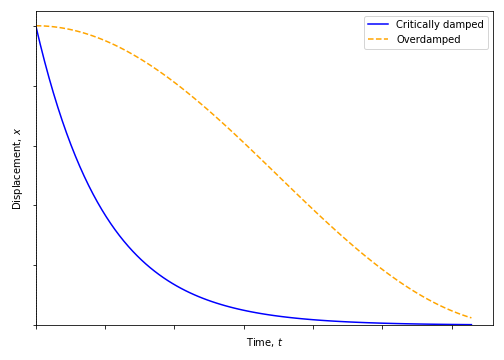
\includegraphics[width=0.7\linewidth]{visualisations/ch4-critoverdamp1} 

}

\caption{A critically damped system returns to its equilbrium position in the shortest possible time, while an overdamped system works against an overbearing damping force slowly returning it to its equilibrium position.}\label{fig:ch4-critvsoverdamped1}
\end{figure}

In the overdamped case, the damping coefficient, \(b\) is greater than the critical damping coefficient, \(b_c\):

\begin{equation}
b > b_c
\end{equation}

\hypertarget{sec:ch4-qualityfactor}{%
\section{Quality factor and energy in damped SHM}\label{sec:ch4-qualityfactor}}

Recall that we determined energies within SHM in Equations \eqref{eq:ch1-potentialfromforce4} and \eqref{eq:ch1-potentialfromforce5}; remembering that \(\omega^2 = \frac{k}{m}\), we can write the overall energy of the system as in Equation \eqref{eq:ch4-qualityfactorenergy1}:

\begin{equation}
E = \frac{1}{2}m\omega^2 A^2
\label{eq:ch4-qualityfactorenergy1}
\end{equation}

Within the damped regimes we have established the equations for damping, in particular how to calculate the damped amplitude at a given time, \(A\) (Equation \eqref{eq:ch4-ampexpdecay1}). By combining this with Equation \eqref{eq:ch4-qualityfactorenergy1} we can obtain an expression for the damped energy, \(E\), as a proportion of the initial energy of the system, \(E_0\) (Equation \eqref{eq:ch4-qualityfactorenergy2}):

\begin{equation}
\begin{array}{rcl}
E &=& \frac{1}{2}m\omega^2 \left( A_0 \mathrm{e}^{-\frac{t}{2\tau}} \right)^2\\
 &=& E_0 \mathrm{e}^{-\frac{t}{\tau}}
\end{array}
\label{eq:ch4-qualityfactorenergy2}
\end{equation}

The decay time \(\tau\) can now be considered the time taken for the energy to decrease to \(\frac{1}{\mathrm{e}}\) of its original value (see? There was a reason we considered the timescale \(2\tau\) in Section \ref{sec:ch4-generalcasedamping}).

A useful measure of the \textbf{persistence} of an oscillation is the \textbf{quality factor}, \(Q\). This is defined as shown in Equation \eqref{eq:ch4-qualityfactor1}:

\begin{equation}
Q = \omega_0 \tau = \frac{\omega_0 m}{b}
\label{eq:ch4-qualityfactor1}
\end{equation}

Generally:

\begin{itemize}
\tightlist
\item
  Large \(Q\) represents lighter damping, persistent oscillation. (think \textbf{high quality oscillation})
\item
  Small \(Q\) represents heavier damping, oscillation stops rapidly. (think \textbf{low quality oscillation})
\end{itemize}

\(Q\) can relate to the energy loss per cycle of oscillation; firstly define the rate of change of energy (Equation \eqref{eq:ch4-qualityfactor2}, from Equation \eqref{eq:ch4-qualityfactorenergy1}):

\begin{equation}
\frac{\mathrm{d}E}{\mathrm{d} t} = -\frac{E_0}{\tau} \mathrm{e}^{-\frac{t}{\tau}} = -\frac{E}{\tau}
\label{eq:ch4-qualityfactor2}
\end{equation}

If we are considering finite changes, we can adapt our calculus to allow \(\Delta E \approx \mathrm{d}E\) and \(\Delta t \approx \mathrm{d}t = T\). Applying this to Equation \eqref{eq:ch4-qualityfactor2} and rearranging gives:

\begin{equation}
\frac{|\Delta E|}{E} = \frac{T}{\tau} = \frac{2 \pi}{\omega_0 \tau} = \frac{2 \pi}{Q}
\end{equation}

This gives us the result for \(Q\) shown in Equation \eqref{eq:ch4-qualityfactor3}:

\begin{equation}
Q = \frac{2 \pi}{\left( \frac{|\Delta E|}{E} \right)_{\mathrm{cycle}}}
\label{eq:ch4-qualityfactor3}
\end{equation}

This gives us one more way to consider the quality factor: it is inversely proportional to the fractional energy loss per cycle of the oscillation. A low \(Q\) therefore corresponds to a higher fractional energy loss per cycle than a high \(Q\) factor.

\hypertarget{sec:ch5-forcedoscillations}{%
\chapter{Forced oscillations}\label{sec:ch5-forcedoscillations}}

\emph{Textbook link: Tipler and Mosca 14.5}

In Chapter \ref{sec:ch4-dampedoscillations} we explored the effect of damping on a system and we said that every system in the real world is, to a greater or lesser extent, a damped system in which energy is lost (dissipated) to the surroundings. In order to maintain the amplitude of any oscillation we must supply energy to the system at the same rate as it is lost to the surroundings; for example, pushing a child on a swing.

The equation for forced SHM is given in Equation \eqref{eq:ch5-forcedshm1}:

\begin{equation}
m \frac{\mathrm{d}^2 x}{\mathrm{d}t^2} + b \frac{\mathrm{d}x}{\mathrm{d}t}+ kx = F_0 \mathrm{e}^{\mathrm{i}\omega t}
\label{eq:ch5-forcedshm1}
\end{equation}

Compare this to Equation \eqref{eq:ch4-velocitydamp3} for damped SHM; we have now applied an oscillating force represented as \(F_0 \mathrm{e}^{\mathrm{i}\omega t}\), with an amplitude of \(F_0\) and frequency \(\omega\). Note that this driving frequency \(\omega\) is different to the natural \emph{undamped} frequency of the oscillator, \(\omega_0 = \sqrt{\frac{k}{m}}\) and different again to the frequency of the damped \emph{unforced} oscillator, \(\omega^\prime = \sqrt{\omega_0^2 - \frac{b^2}{4m^2}}\).

Any forced oscillation consists of two distinct regimes:

\begin{enumerate}
\def\labelenumi{\arabic{enumi}.}
\tightlist
\item
  An initial transient period during which the oscillations are established, and
\item
  A steady state period during which the oscillations have constant amplitude and a frequency equal to the driving frequency, \(\omega\).
\end{enumerate}

The general solution of the equation for forced SHM shown in Equation \eqref{eq:ch5-forcedshm1} is a combination of these two regimes.

\hypertarget{sec:ch5-transientsolution}{%
\section{The Transient Solution}\label{sec:ch5-transientsolution}}

The solution to the transient component of the forced oscillator is identical to the solution of damped SHM (\emph{i.e.} Equation \eqref{eq:ch5-forcedshm1} with the right-hand side set to zero; identical to Equation \eqref{eq:ch4-velocitydamp3}). Its solution is shown in Equation \eqref{eq:ch5-forcedshm2}:

\begin{equation}
\begin{array}{lrcl}
 & x &=& A_0 \mathrm{e}^{- \left(\frac{b}{2m}\right)t} \mathrm{e}^{\mathrm{i} \left( \omega^\prime t + \delta^\prime \right)} \\
\textsf{or:} & x &=& A_0 \mathrm{e}^{- \left(\frac{b}{2m}\right)t} \cos \left( \omega^\prime t + \delta^\prime \right) \\
\end{array}
\label{eq:ch5-forcedshm2}
\end{equation}

This contribution to motion establishes the oscillation, but rapidly decays with time constant \(\tau = \frac{m}{b}\). The term \(\delta^\prime\) is simply the phase constant for this transient oscillation.

\hypertarget{sec:ch5-steadystatesolution}{%
\section{The Steady State solution}\label{sec:ch5-steadystatesolution}}

Once in the steady state, the energy which is put into the system during each cycle is equal to the energy dissipated per cycle due to the damping in the system. If there is no damping of the system, energy keeps being added to the system and the amplitude will increase indefinitely. This is \textbf{not} a steady state, and is an \textbf{unphysical result}. The frequency then of this `driven' oscillator in the steady state is equal to the driving frequency.

The amplitude (and hence the energy) of the system in the steady state depends on both the \textbf{amplitude} and the \textbf{frequency} of the driving force. For a steady state, the solution to Equation \eqref{eq:ch5-forcedshm1} is in the form shown in Equation \eqref{eq:ch5-forcedshm3}:

\begin{equation}
x = A \mathrm{e}^{\mathrm{i}\left(\omega t - \delta \right)}
\label{eq:ch5-forcedshm3}
\end{equation}

The terms \(A\) and \(\delta\) are defined in Equations \eqref{eq:ch5-forcedshm4} and \eqref{eq:ch5-forcedshm5} below:

\begin{equation}
A = \frac{F_0}{\sqrt{m^2 \left(\omega_0^2 - \omega^2 \right)^2 + b^2 \omega^2}}
\label{eq:ch5-forcedshm4}
\end{equation}

\begin{equation}
\delta = \arctan \left( \frac{b\omega}{m \left(  \omega_0^2 - \omega^2 \right)} \right)
\label{eq:ch5-forcedshm5}
\end{equation}

\hypertarget{sec:ch5-steadystatebehaviour}{%
\section{Steady state behaviour - Resonance}\label{sec:ch5-steadystatebehaviour}}

When we vary the frequency of the driving frequency we find that the response of the driven system varies. If we examine the power transferred to the system as we vary the driving frequency, we see that there is a peak around the natural frequency, \(\omega_0\), of the driven system (Figure \ref{fig:ch5-resonancepowerfrequency1}). This is a phenomenon known as \textbf{resonance}.

\begin{figure}

{\centering 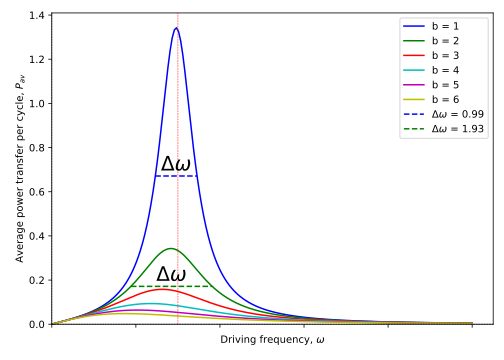
\includegraphics[width=0.7\linewidth]{visualisations/ch5-forcedosc2} 

}

\caption{The power transferred to a system varies with the driving frequency. The power transferred to a system is proportional to $\omega A^2$. The full-width at half-maximum value is designated $\Delta \omega$. Note that as the damping coefficient $b$ increases, there is a shift in maximum power transmission away from the natural frequency $\omega_0$.}\label{fig:ch5-resonancepowerfrequency1}
\end{figure}

If this system is damped, we also see a change in the ``full-width at half-maximum'' value.\footnote{The ``full-width at half maximum'' (FWHM) is a term widely used in signals processing to describe the ``spread'' of a signal. A large FWHM indicates a broad signal over a range of frequencies, while a small FWHM indicates a sharp signal over a narrow band of frequencies.} This FWHM is designated by \(\Delta \omega\) in Figure \ref{fig:ch5-resonancepowerfrequency1} and is related to the \(Q\)-factor of the system via Equation \eqref{eq:ch5-resonancequality1}:

\begin{equation}
\frac{\Delta \omega}{\omega_0} = \frac{1}{Q}
\label{eq:ch5-resonancequality1}
\end{equation}

This allows us to determine the \(Q\)-factor of a system through measurement of resonance of the system, as a lightly-damped system (high \(Q\)) will give a sharp resonance with low \(\Delta \omega\), while a more heavily damped system will lead to a more broad resonance profile.

This use of the \(Q\)-factor is important as it give us a measure of the `sharpness' (or quality) of the resonance. It may be applied ot many systems including electronic circuits.

We can also examine the phase of the oscillator's displacement \(x\) relative to that of the driving force, \(\delta\), shown in Figure \ref{fig:ch5-resonancephaseshift1}.

\begin{figure}

{\centering 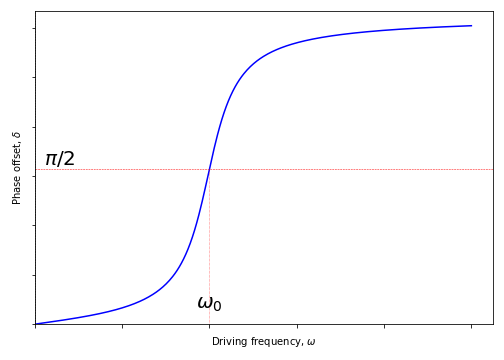
\includegraphics[width=0.7\linewidth]{visualisations/ch5-forcedosc3} 

}

\caption{The phase shift $\delta$ of the observed oscillation varies relative to the driving frequency $\omega$.}\label{fig:ch5-resonancephaseshift1}
\end{figure}

We can see that at low driving frequencies, there is very little phase shift between the two (the force is at a minimum when the displacement is at a minimum and is in the same direction), while at very high driving frequencies we approach a maximum phase shift of \(\frac{\pi}{2}\) between the two (force still at a minimum at minimum displacement, but now the force is directed in the opposite direction to the displacement; akin to SHM). The phase change is at its most rapid when the frequency of the driving force \(\omega\) is similar to the natural frequency of the oscillator (\(\omega_0\)). At this point, the driving force are ``in quadrature'' (90\(^\circ\) out of phase), with the force at a maximum when \(x\) is changing most rapidly.

\hypertarget{sec:ch5-fullsolutionforcedoscillator}{%
\section{Full solution of the forced oscillator}\label{sec:ch5-fullsolutionforcedoscillator}}

As with the damped oscillator explored in Chapter \ref{sec:ch4-dampedoscillations}, the full solution of the forced oscillator is found through the combination of the ``transient state'' (a free, damped system) and the ``steady state'' (fully forced oscillations). This is illustrated in Equation \eqref{eq:ch5-forcedoscillfullsoln1}:

\begin{equation}
\begin{array}{lrcccc}
& x &=& \textsf{transient} &+&\textsf{steady state} \\
\textit{i.e.} & x&=& A_0 \mathrm{e}^{- \left(\frac{b}{2m}\right)t} \mathrm{e}^{\mathrm{i} \left( \omega^\prime t + \delta^\prime \right)} &+&  A \mathrm{e}^{\mathrm{i}\left(\omega t - \delta \right)} \\
\end{array}
\label{eq:ch5-forcedoscillfullsoln1}
\end{equation}

The terms in Equation \eqref{eq:ch5-forcedoscillfullsoln1} are as follows:

\begin{itemize}
\tightlist
\item
  \(\delta\) is given by Equation \eqref{eq:ch5-forcedshm5};
\item
  \(A\) given by Equation \eqref{eq:ch5-forcedshm4};
\item
  \(A_0\) and \(\delta^\prime\) depend on the initial conditions;
\item
  \(\omega\) is the driving frequency;
\item
  \(\omega^\prime\) is the frequency of the damped (transient) oscillations.
\end{itemize}

We can simplify our view of Equation \eqref{eq:ch5-forcedoscillfullsoln1} by applying initial conditions whereby the displacement \(x = 0\) at time \(t = 0\). Therefore:

\begin{equation}
0 = A_0 \mathrm{e}^{\mathrm{i} \left( \delta^\prime \right)} + A \mathrm{e}^{-\mathrm{i}\delta}
\end{equation}

\ldots or, to rearrange, we obtain the form shown in Equation \eqref{eq:ch5-forcedoscillfullsoln2}:

\begin{equation}
A_0 = -A \mathrm{e}^{-\mathrm{i}\left( \delta + \delta^\prime \right)}
\label{eq:ch5-forcedoscillfullsoln2}
\end{equation}

As with any complex representation, we now compare the \textbf{real} and \textbf{imaginary} parts of the solution. Remember that Equation \eqref{eq:ch5-forcedoscillfullsoln2} expands \emph{via} De Moivre's theorem to:

\begin{equation}
A_0 = -A \left( \cos \left( \delta + \delta^\prime \right) + \mathrm{i} \sin \left( \delta + \delta^\prime \right)  \right)
\label{eq:ch5-forcedoscillfullsoln3}
\end{equation}

The imaginary component of Equation \eqref{eq:ch5-forcedoscillfullsoln3} reduces to zero (the solution, \(A_0\) is fully real):

\begin{equation}
0 = -A \sin \left( \delta + \delta^\prime \right)
\end{equation}

We can therefore relate \(\delta\) and \(\delta^\prime\) as follows:

\begin{equation}
\begin{array}{rcl}
\delta + \delta^\prime = \pi & \textit{i.e.} & \delta^\prime = \pi - \delta
\end{array}
\label{eq:ch5-forcedoscillationfullsoln4}
\end{equation}

We now examine the `real' component of Equation \eqref{eq:ch5-forcedoscillfullsoln3}, equal to \(A_0\):

\begin{equation}
A_0 = - A \cos \left( \delta + \delta^\prime \right)
\end{equation}

\ldots and doing the same analysis, now that we know that, under our initial conditions, \(\delta + \delta^\prime = \pi\):

\begin{equation}
\begin{array}{rcl}
A_0 = -A \cos \pi & \textit{i.e.} & A_0 = A
\end{array}
\label{eq:ch5-forcedoscillationfullsoln5}
\end{equation}

We can now revisit Equation \eqref{eq:ch5-forcedoscillfullsoln1}, now that we have values for \(\delta\), \(\delta^\prime\) and \(A_0\) under our starting conditions ( \(x = 0\) when \(t = 0\)):

\begin{equation}
\begin{array}{rcl}
x &= & A \left[ \mathrm{e}^{\mathrm{i}\left(\omega t - \delta \right)}  + \mathrm{e}^{- \left(\frac{b}{2m}\right)t} \mathrm{e}^{\mathrm{i} \left( \omega^\prime t + \delta^\prime \right)} \right]\\

&= & A \left[ \mathrm{e}^{\mathrm{i}\left(\omega t - \delta \right)}  + \mathrm{e}^{- \left(\frac{b}{2m}\right)t} \mathrm{e}^{\mathrm{i} \left( \omega^\prime t + \pi - \delta \right)} \right]\\

&= & A \left[ \mathrm{e}^{\mathrm{i}\left(\omega t - \delta \right)}  + \mathrm{e}^{- \left(\frac{b}{2m}\right)t} \mathrm{e}^{\mathrm{i} \left( \omega^\prime t - \delta \right)} \mathrm{e}^{\mathrm{i} \pi} \right]\\

&= & A \left[ \mathrm{e}^{\mathrm{i}\left(\omega t - \delta \right)}  - \mathrm{e}^{- \left(\frac{b}{2m}\right)t} \mathrm{e}^{\mathrm{i} \left( \omega^\prime t - \delta \right)}  \right]\\

\end{array}
\label{eq:ch5-forcedoscillationfullsoln6}
\end{equation}

Finally, we can find the actual displacement of the oscillator by examining the real component of Equation \eqref{eq:ch5-forcedoscillationfullsoln6}, summarised in Equation \eqref{eq:ch5-forcedoscillationfullsoln7}:

\begin{equation}
\mathrm{Re}(x) = A \left[ \cos (\omega t - \delta) - \mathrm{e}^{- \left(\frac{b}{2m}\right)t} \cos (\omega^\prime t - \delta) \right]
\label{eq:ch5-forcedoscillationfullsoln7}
\end{equation}

We can visualise the amplitude of a forced oscillator, as shown in Figure \ref{fig:ch5-forcedoscilfull1}. At very low frequencies, the oscillation has the same amplitude as the driving oscillation. This rapidly increases under resonance to a peak, but then drops rapidly to a value towards zero.

\begin{figure}

{\centering 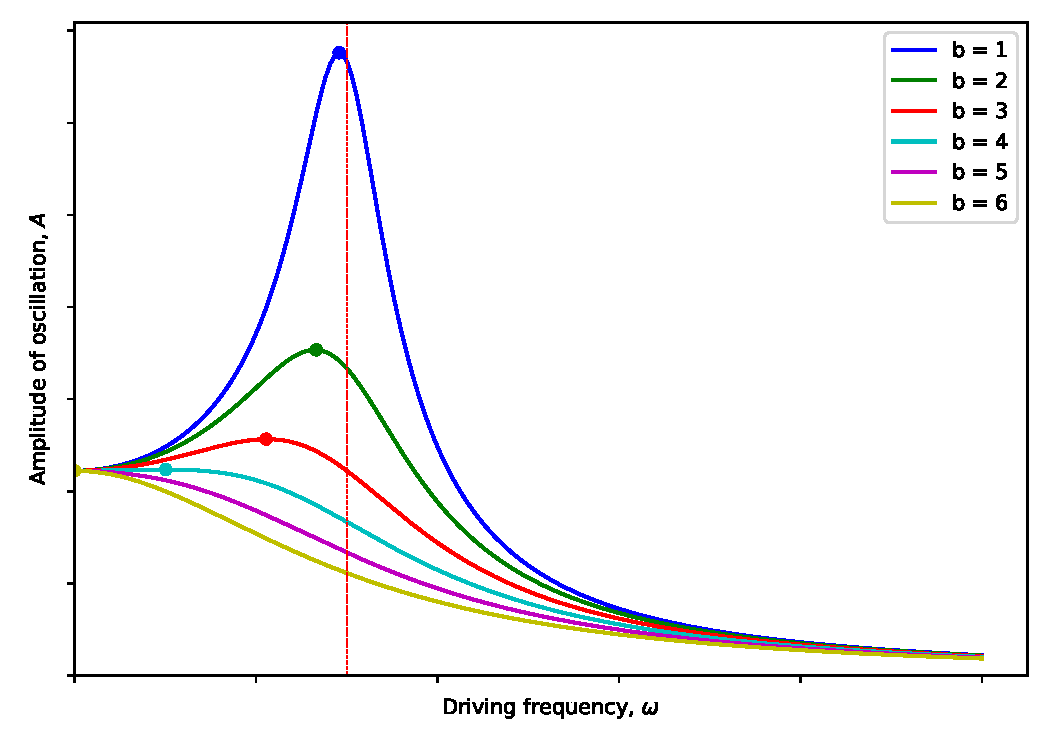
\includegraphics[width=0.7\linewidth]{visualisations/ch5-forcedosc1} 

}

\caption{The amplitude of a forced oscillation varies with driving frequency; close to the driving amplitude at very low frequencies, close to zero at very high frequencies, with a peak occurring under resonant conditions. Note that the position of this peak varies with the damping coefficient $b$.}\label{fig:ch5-forcedoscilfull1}
\end{figure}

Note that the position of the resonant peak amplitude also varies with the damping coefficient \(b\).

\hypertarget{special-cases-of-forced-oscillations}{%
\subsection{Special cases of forced oscillations}\label{special-cases-of-forced-oscillations}}

There are three special cases of forced oscillations to consider:

\begin{enumerate}
\def\labelenumi{\arabic{enumi}.}
\tightlist
\item
  \(\omega \ll \omega_0\)
\item
  \(\omega \gg \omega_0\)
\item
  \(\omega = \omega_0\)
\end{enumerate}

\begin{figure}

{\centering 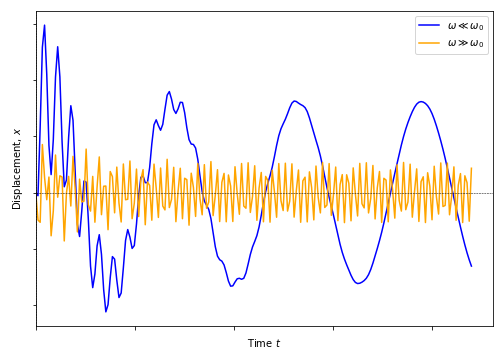
\includegraphics[width=0.7\linewidth]{visualisations/ch5-forcedosc4} 

}

\caption{When the frequency of the driving oscillation $\omega$ is very different to the natural frequency of the system we see two regimes; firstly, where $\omega \ll \omega_0$ (blue), the natural frequency decays and we are left to observe the driving frequency at a large amplitude; when $\omega \gg \omega_0$ (orange), we see a much smaller amplitude oscillation at close to the driving frequency.}\label{fig:ch5-forcedosc4}
\end{figure}

In the special case when \(\omega = \omega_0\) and the damping coefficient \(b\) is small (allowing the damped frequency \(\omega^\prime\) to be approximately equal to the driving frequency \(\omega\)), we can rewrite the expression of the displacement (Equation \eqref{eq:ch5-forcedoscillationfullsoln7}) as shown in Equation \eqref{eq:ch5-forcedoscillationfullsoln8}:

\begin{equation}
\mathrm{Re}(x) = A  \cos (\omega_0 t - \delta) \left[ 1 - \mathrm{e}^{- \left(\frac{b}{2m}\right)t}  \right]
\label{eq:ch5-forcedoscillationfullsoln8}
\end{equation}

We can see that the oscillation will converge to a maximum value, at which point the energy put into the system becomes equal to the energy dissipated by the system through damping, as shown in Figure \ref{fig:ch5-resonancedisplacement1}

\begin{figure}

{\centering 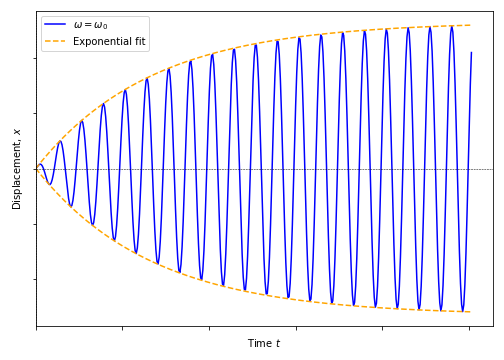
\includegraphics[width=0.7\linewidth]{visualisations/ch5-forcedosc5} 

}

\caption{When the frequency of the driving oscillation $\omega = \omega_0$ (blue), we see the amplitude grow to a plateau at which point the energy put into the system is equal to the energy losses from the system.}\label{fig:ch5-resonancedisplacement1}
\end{figure}

\hypertarget{sec:ch5-energydrivenoscillators}{%
\section{Energy in driven oscillators}\label{sec:ch5-energydrivenoscillators}}

In a driven oscillator, energy is continually added to the system. When it reaches its steady state, the rate of loss of energy in each cycle due to damping of the system is equal to the work done by the driving force.

We can demonstrate this through integration; remember that (simplistically!) work done is ``force \(\times\) distance'', so under varying force (as we have here), we can integrate the force with respect to displacement \(x\) to find an expression for the work done.

For the sake of convenience, we will consider the ``real'' component of the equation for forced SHM shown in Equation \eqref{eq:ch5-forcedshm1} (the left-hand-side is entirely ``real'', so the ``imaginary'' component reduces to zero anyway):

\begin{equation}
m \frac{\mathrm{d}^2 x}{\mathrm{d}t^2} + b \frac{\mathrm{d}x}{\mathrm{d}t}+ kx = F_0 \cos \omega t
\label{eq:ch5-oscillatorenergy1}
\end{equation}

We also know that the steady state solution for the displacement \(x\) in SHM is as given in Equation \eqref{eq:shm-general-positionx1}. We can then find an expression for the velocity \(v\) by finding the first derivative of this expression (Equation \eqref{eq:ch5-oscillatorenergy2}):

\begin{equation}
\begin{array}{rcl}
x& =& A \cos (\omega t - \delta)\\
v = \dfrac{\mathrm{d}x}{\mathrm{d}t} &=& -\omega A \sin (\omega t - \delta)
\end{array}
\label{eq:ch5-oscillatorenergy2}
\end{equation}

\hypertarget{sec:ch5-energyinputdrivenosc}{%
\subsection{Energy input for driven oscillators}\label{sec:ch5-energyinputdrivenosc}}

To find the energy which is put into the system over one cycle, we therefore need to find the integral of the force acting over one cycle of the oscillation, from \(t = 0\) to \(t = T\) (remember that \(T\) is the period of the oscillation). We do this integration by substituting our variable \(\mathrm{d}x\) for \(v\mathrm{d}t\) (as defined in Equation \eqref{eq:ch5-oscillatorenergy2}):

\begin{equation}
\begin{array}{rcl}
E_\mathrm{in} = \displaystyle{\int_0^T} F \cdot \mathrm{d}x &\equiv& \displaystyle{\int_0^T} F \cdot v \mathrm{d}t \\
&=& \displaystyle{\int_0^T} F_0 \cos \omega t \cdot \left[ -\omega A \sin (\omega t + \delta)\right] \mathrm{d}t \\
&=& -\omega A F_0 \displaystyle{\int_0^T} \cos \omega t \cdot \sin (\omega t + \delta) \\
&=& -\omega A F_0 \displaystyle{\int_0^T} \cos \omega t \cdot \left[ \sin \omega t \cos \delta + \cos \omega t \sin \delta  \right] \\
&=& -\omega A F_0 \displaystyle{\int_0^T} \left[ \cos \omega t \sin \omega t \cos \delta + \cos \omega t \cos \omega t \sin \delta \right] \\
&=& -\omega A F_0 \displaystyle{\int_0^T} \left[ \tfrac{1}{2} \sin 2\omega t \cos \delta + \left( \tfrac{1}{2}\cos 2\omega t + \tfrac{1}{2} \right) \sin \delta \right] \\
&=& -\omega A F_0 \left[ -\tfrac{1}{4\omega} \cos 2\omega t \cos \delta  + \left( \tfrac{1}{4\omega}\sin 2\omega t + \tfrac{t}{2} \right)\sin \delta \right]_0^T\\
&=& -\omega A F_0 \left( \left[ -\tfrac{1}{4\omega} \cos 2\omega T \cos \delta  + \left( \tfrac{1}{4\omega}\sin 2\omega T + \tfrac{T}{2} \right)\sin \delta \right] - \left[ -\tfrac{1}{4\omega} \cos 0 \cos \delta  + \left( \tfrac{1}{4\omega}\sin 0 + \tfrac{0}{2} \right)\sin \delta \right] \right)  \\

\end{array}
\end{equation}

Evaluation of this integral gives us the end result shown in Equation\eqref{eq:ch5-oscillatorenergy4}:

\begin{equation}
E_{\mathrm{in}} = \frac{1}{2}\omega A F_0 T \sin \delta
\label{eq:ch5-oscillatorenergy4}
\end{equation}

If we recall that \(\delta = \frac{\pi}{2}\) at resonance, substitution of this value into Equation \eqref{eq:ch5-oscillatorenergy4} tells us that the maximum energy is transferred to the oscillator when driven at a resonant frequency - in line wiht our expectations.

If we now use the definition of \(\delta\) in Equation \eqref{eq:ch5-forcedshm5}, we can use trigonometry and the expression for \(A\) in Equation \eqref{eq:ch5-forcedshm4} to give the expression \(\sin \delta = \frac{Ab\omega}{F_0}\); we can also use the fact that the period of oscillation \(T\) and the angular frequency \(\omega\) are related by Equation \eqref{eq:ch1-definingomega1} (\(T = \frac{2\pi}{\omega}\)), and simplify the expression for the energy input for the forced oscillator as shown in Equation \eqref{eq:ch5-oscillatorenergy5}:

\begin{equation}
E_{\mathrm{in}} = \pi b \omega A^2
\label{eq:ch5-oscillatorenergy5}
\end{equation}

\hypertarget{sec:ch5-energylostdrivenosc}{%
\subsection{Energy lost in driving oscillators}\label{sec:ch5-energylostdrivenosc}}

To now determine the amount of energy, we follow a similar process as followed in Section \ref{sec:ch5-energyinputdrivenosc}. This time however we need to determine the work done by the oscillator on the damping force during one cycle. This integral is set up as follows:

\begin{equation}
E_{\mathrm{lost}} = \int_0^T F v \mathrm{d}t
\end{equation}

\ldots but this time the force is the damping force, \(F_{\mathrm{damp}} = bv\).

\begin{equation}
E_{\mathrm{lost}} = \int_0^T b v^2 \mathrm{d}t
\end{equation}

As before, we have the result that \(v = -\omega A \sin(\omega t - \delta)\) (Equation \eqref{eq:ch5-oscillatorenergy2}), and followign through the integration in a similar manner as in the previous section we are led to the result in Equation \eqref{eq:ch5-oscillatorenergy6} for a \textbf{driven damped oscillator} at \textbf{steady state}.

\begin{equation}
E_{\mathrm{lost}}  = \pi b \omega A^2= E_{\mathrm{in}}
\label{eq:ch5-oscillatorenergy6}
\end{equation}

This result should not be a surprise; at a steady state, we expect the energy lost to be equivalent to the energy put into the system, however it is nice that this is vindicated through the mathematics!

A similar result may be obtained for electrical systems in resonance.

\textbf{Note}: When \(b = 0\) the above result appears to fail (no energy is lost, but none is put in??); in fact, in an undamped system there can be no steady state (as no energy is lost!), so the amplitude of vibration \(A \rightarrow \infty\), so this result does not apply.

\hypertarget{sec:ch5-impedance}{%
\section{Impedance}\label{sec:ch5-impedance}}

As you learn about fields, you will examine electrical circuits and see that circuits contaning capacitors and indutors are analogous to mechanical oscillators, with the electrical charge oscillating within the circuit. These properties of circuits have many important applications and you will find that much of the analysis we have done here can be applied to those electrical systems.

In the context of an electrical circuit it is useful to define the term \textbf{impedance} a measure of the opposition to the flow of current, and is defined as the ratio of the voltage to current (\(\frac{V}{I}\)) for a particular circuit component. For a resistor this is simply the resistance, however capacitors and inductors also possess impedence.

It turns out to be helpful to write this impedance as a complex number with components in both the real and imaginary plane. This works well with the complex representation of oscillations and naturally takes care of any differences in phase of the current and voltage in different components.

Bringing the analogy back to mechanical oscillations, a mechanical system can also be considered to have an impedence. We define the mechanical impedance as the \textbf{force required to produce unit velocity}, \emph{i.e.} \(Z_m = \frac{F}{v}\), or \(F = vZ_m\). This is the mechanical equivalent of Ohm's law; force corresponding to the voltage, and velocity corresponding to current.

This idea of mechanical impedance will be useful in discussion of wave propagation.

\hypertarget{sec:ch6-wavemotion}{%
\chapter{Simple wave motion and the Wave Equation}\label{sec:ch6-wavemotion}}

\emph{Textbook link: Tipler and Mosca, Section 15.1}

A wave is a means by which energy and momentum are carried through space, without transporting matter. When we consider a medium which carries a wave, the particles of that material oscillate about a mean position, but have an average displacement of zero; \emph{i.e.} they always return to their starting position. A wave can be of any shape - there is no requirement for a wave to be sinusoidal, though this is the simplest shape which we can consider mathematically.

We also consider waves to be either \textbf{transverse}; where the displacement of the medium is perpendicular to the direction of wave propagation (\emph{e.g.} a wave travelling along a string), or they can be \textbf{longitudinal}; where the displacement of the medium is parallel to the direction of propagation (\emph{e.g.} a sound wave passing through air).

\begin{figure}

{\centering 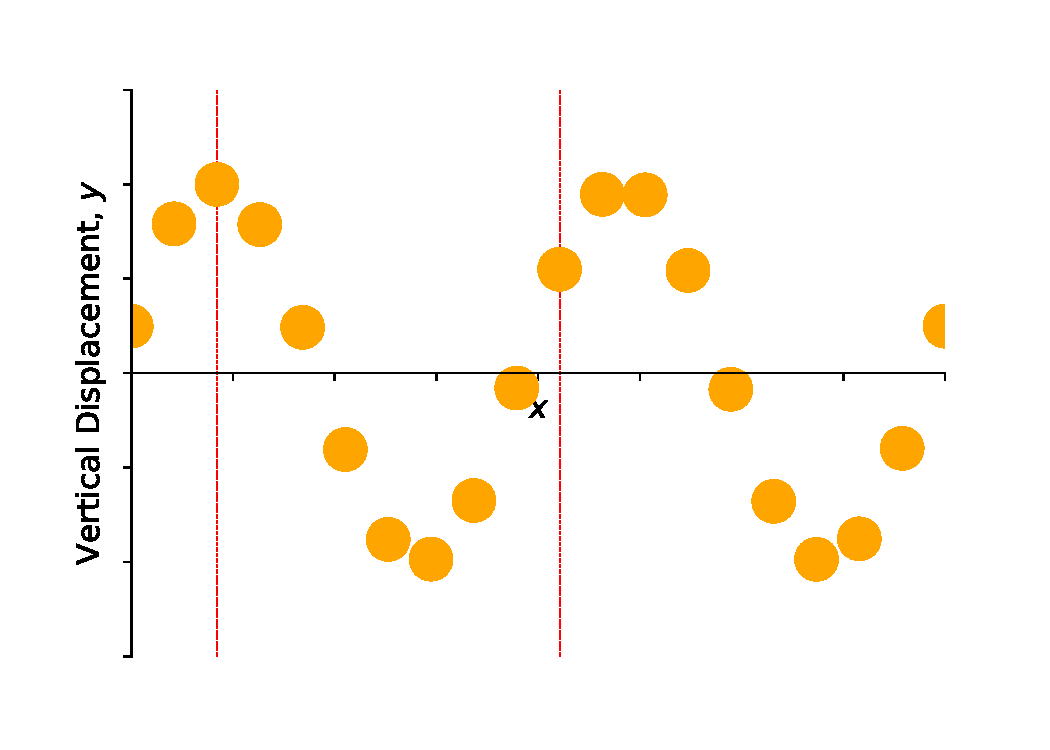
\includegraphics[width=0.7\linewidth]{visualisations/ch6-transversewave2} 

}

\caption{An animation to show the propagation of a wave through a material arising from an organised transverse oscillation of many particles. The two marked particles only move up and down, but the net effect of the organised motion is a propagation of energy to the right.}\label{fig:ch6-transversewaveill1}
\end{figure}

\begin{figure}

{\centering 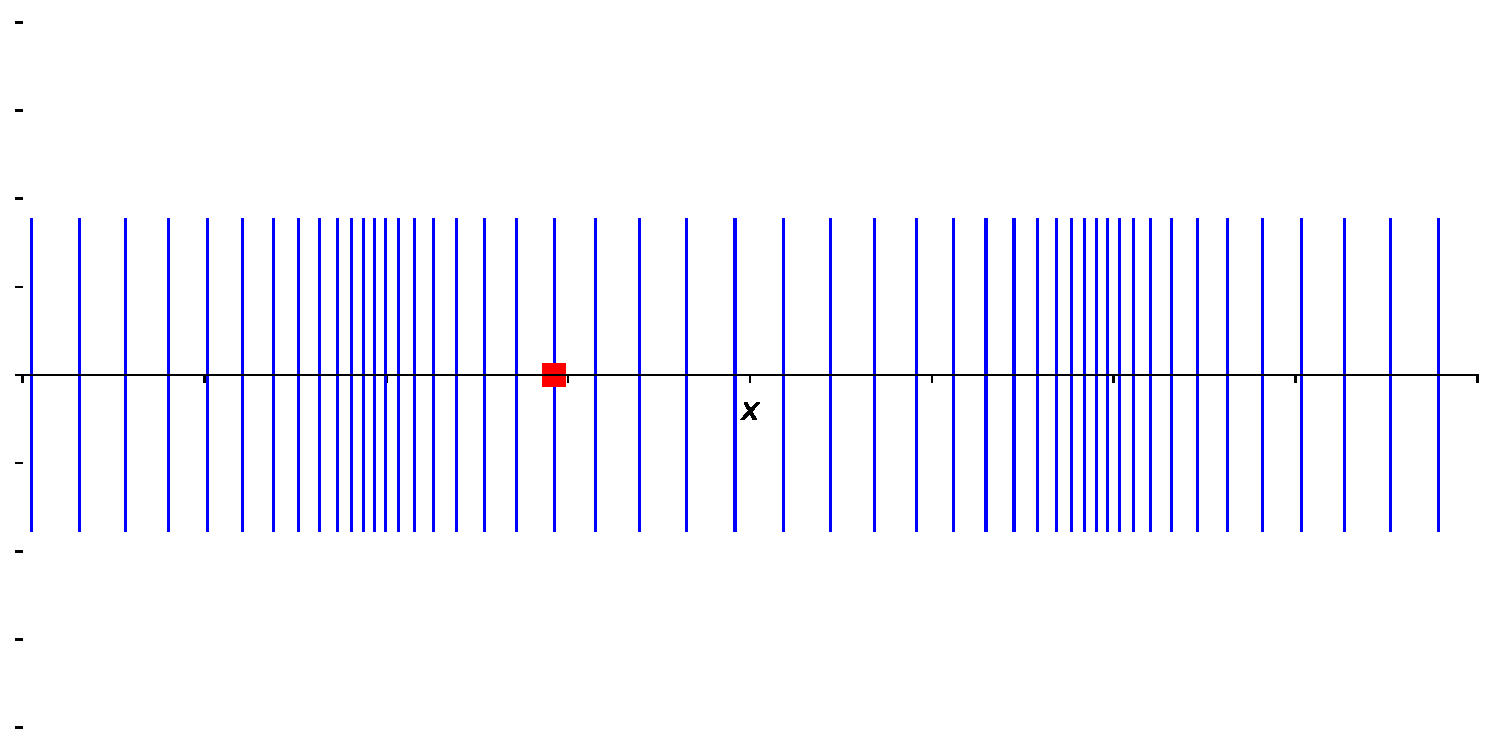
\includegraphics[width=0.7\linewidth]{visualisations/ch6-longitudinalwave1} 

}

\caption{An animation to show the propagation of a wave through a material arising from an organised longitudinal oscillation of many particles. The marked particle now  moves in the direction of propagation, but oscillates around a fixed point; the net effect of the organised motion is again a propagation of energy to the right.}\label{fig:ch6-longitudinalwaveill1}
\end{figure}

\hypertarget{a-note-on-transverse-waves}{%
\subsection*{A note on transverse waves}\label{a-note-on-transverse-waves}}
\addcontentsline{toc}{subsection}{A note on transverse waves}

In contrast with longitudinal waves, the medium carrying a transverse wave is displaced perpendicular to the direction of travel. This gives rise to the phenomenon of \textbf{polarisation}. A \emph{plane of polarisation} is defined as a plane containing the displacement direction and the direction of propagation. For any given transverse wave, two orthogonal independent polarisations are possible. All other polarisations may be constructed from weighted combinations of these two basic polarisations. For electromagnetic waves, it is the \textbf{electric field vector} which defines the plane of polarisation in combination with the direction of propagation. We will revisit these properties of transverse waves as we go through our discussion.

\hypertarget{sec:ch6-wavepulses}{%
\section{Wave pulses}\label{sec:ch6-wavepulses}}

Where a wave is a sustained periodic disturbance which propagates energy through a medium, a \textbf{wave pulse} in contrast is any localised non-periodic disturbance propagating an energy pulse through the medium. A typical pulse is shown in Figure \ref{fig:ch6-wavepulse1}.

\begin{figure}

{\centering 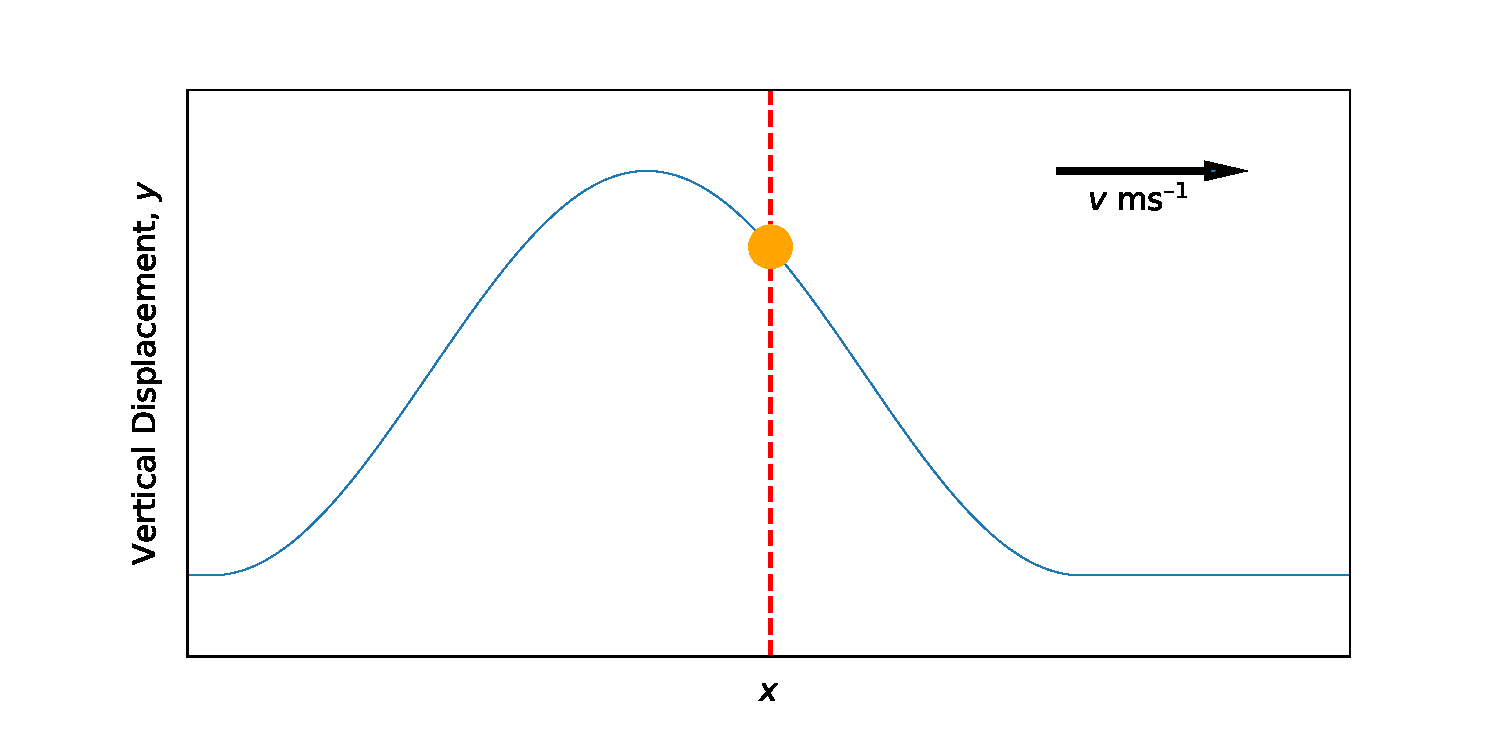
\includegraphics[width=0.7\linewidth]{visualisations/ch6-wavepulse1} 

}

\caption{A wave pulse propagating through a system at velocity $v$; this causes a temporary transverse disturbance of molecules in the system from their origin.}\label{fig:ch6-wavepulse1}
\end{figure}

We illustrate a pulse graphically as any function defined as \(y = f(x)\), where the \(+x\) direction is the direction of propagation of the pulse. If the pulse propagates without changing shape, it becomes convenient to consider a moving reference frame within which the pulse is stationary; \emph{i.e.} rather than imagining the pulse moving to the right along fixed axes, we keep the pulse stationary in our view and move the axes to the left.

In the moving frame then, the pulse is described as \(y^\prime = f(x^\prime)\) for all times, because the pulse does not change its shape.

We can interconvert between the two frames of reference by the relation:

\begin{equation}
x = x^\prime + vt
\label{eq:ch6-refframeconvert1}
\end{equation}

\ldots where \(v\) is the velocity of the pulse. This allows us to convert the position in the moving reference frame, \(x^\prime\), back to the position in the fixed reference frame by adding the distance \(vt\).

\begin{figure}

{\centering 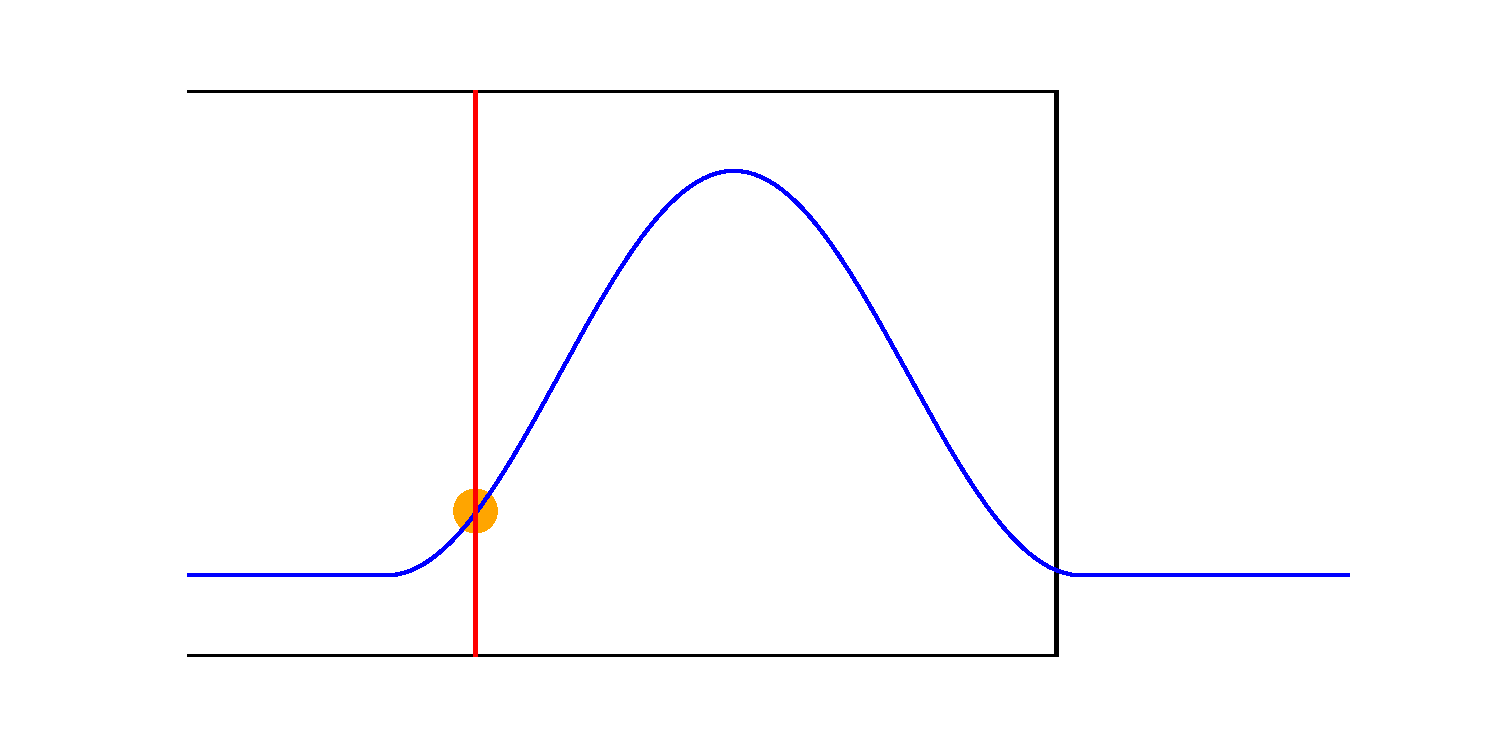
\includegraphics[width=0.7\linewidth]{visualisations/ch6-wavepulse2} 

}

\caption{Rather than imagining a moving wave pulse, we can consider it from the reference frame of the wave pulse; in this example the wave pulse is stationary, but the space moves past it.}\label{fig:ch6-referenceframes1}
\end{figure}

\begin{figure}

{\centering 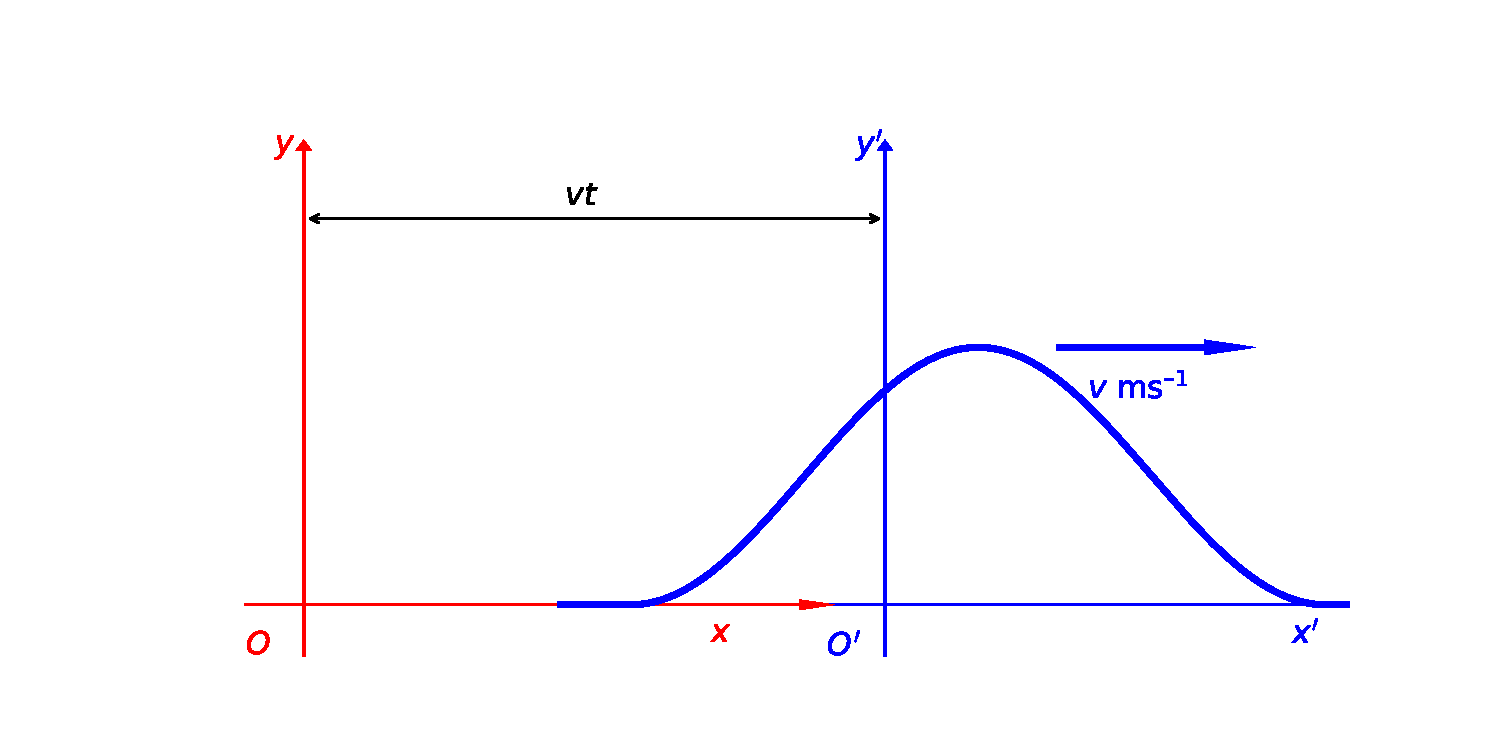
\includegraphics[width=0.7\linewidth]{visualisations/ch6-wavepulse3} 

}

\caption{Another way of visualising the reference frames is to consider the $x',y'$ space moving relative to the stationary $x,y$ space; the offset between them can then be quantified as $vt$, where $v$ is the velocity of the wave pulse and $t$ is the time elapsed.}\label{fig:ch6-referenceframes2}
\end{figure}

If the shape of the pulse in the moving frame is defined as \(y^\prime = f(x^\prime)\) we can use Equation \eqref{eq:ch6-refframeconvert1} to find the shape of the pulse in the static frame, \(y\):

\begin{equation}
\begin{array}{rcl}
y &=& f(x^\prime)\\
&=& f(x - vt)
\end{array}
\label{eq:ch6-refframeconvert2}
\end{equation}

The relation described in Equation \eqref{eq:ch6-refframeconvert2} describes a wave moving to the \textbf{RIGHT}; for a pulse moving to the \textbf{left}, \(v\) becomes negative, and hence:

\begin{equation}
y = f(x + vt)
\end{equation}

The function \(y = f(x \pm vt)\) is known as the \textbf{wave function}; it describes the displacement of the medium, whether the transverse displacement of a string or the longitudinal displacement of air molecules in a sound wave.\footnote{It may seem counterintuitive that, for a wave moving with positive \(v\)in the \(+x\) direction, we subtract \(vt\); but try thinking this way: after time \(t\), the wave will have advanced further to the right. If, after one second, the shape of the wave has its peak at \(x_a\), after three seconds, the peak will have advanced to \(x_b = x_a + vt\); \textbf{however}, the value of the wavefunction at \(x_a\) at this new time (\(x_a^\prime\)) will have come from the value of the wavefunction three seconds earlier, to the \textbf{left} of the point; i.e.~\(x_a^\prime = x_a - vt\)}.

The \emph{wave function} is a solution of the \textbf{wave equation} (Equation \eqref{eq:ch6-waveequation1}):\footnote{The \(\partial\) symbol refers to \emph{partial differentiation}.}

\begin{equation}
\frac{\partial^2 y}{\partial x^2} = \frac{1}{v^2} \frac{\partial^2 y}{\partial t^2}
\label{eq:ch6-waveequation1}
\end{equation}

\textbf{Any} function in the form \(y = f(x \pm vt)\) is a solution of this wave equation; \emph{i.e.} the wave equation describes the uniform propagation of \textbf{any} displacement, provided it does not change shape as it travels. There are numerous examples of such functions, including:

\begin{itemize}
\tightlist
\item
  \(y = \exp(x-vt)^2\)
\item
  \(y = \frac{\sin(x-vt)}{x-vt}\)
\item
  \(y = \cos (x+vt)\)
\end{itemize}

\hypertarget{sec:ch6-derivingwaveequation}{%
\section{Deriving the wave equation}\label{sec:ch6-derivingwaveequation}}

To better understand the wave equation, it is useful to know its derivation. To do this, we shall first consider a segment of string from a curved part of a wave pulse (Figure \ref{fig:ch6-waveeqnderiv1}):

\begin{figure}

{\centering 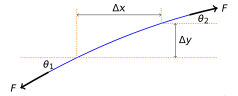
\includegraphics[width=0.7\linewidth]{visualisations/LaTeX/ch6-waveequationderiv1} 

}

\caption{Here we consider a small portion of a string carrying a wave pulse; the tension in the string $F$ is constant throughout, but resolving the forces via the angles $\theta_1$ and $\theta_2$ allows us to determine the equation of motion on this segment. }\label{fig:ch6-waveeqnderiv1}
\end{figure}

The length of this segement is \(\approx \Delta x\) (for small angles), and the mass of this segment of string \(m = \mu \Delta x\) (where \(\mu\) is the mass per unit length). As we are considering a transverse wave, this segment of string will move vertically, and all forces acting on the segment arise from the tension force within the string. We can determine these forces by resolving the horizontal and vertical components of this force \(F\) using the parameters laid out in Figure \ref{fig:ch6-waveeqnderiv1}.

By considering the net vertical force acting on this segment:

\begin{equation}
\begin{array}{rcll}
\sum F &=& F \sin \theta_2 - F \sin \theta_1 &\\
&=& F \left( \tan \theta_2 - \tan \theta_1 \right) & \textsf{for small angles}
\end{array}
\label{eq:ch6-waveeqnderiv1}
\end{equation}

We can also determine an expression for the slope, \(S\), of the segment of string at a given point:

\begin{equation}
S = \tan \theta = \frac{\partial y}{\partial x}
\label{eq:ch6-waveeqnderiv2}
\end{equation}

This means we can now express the overall force acting on the segment in terms of the slope of the segment at its start and end points (assuming small angles!) by combining Equations \eqref{eq:ch6-waveeqnderiv1} and \eqref{eq:ch6-waveeqnderiv2} :

\begin{equation}
\sum F = F(S_2 - S_1) = F \Delta S
\label{eq:ch6-waveeqnderiv3}
\end{equation}

The quantity \(F\Delta S\) in Equation \eqref{eq:ch6-waveeqnderiv3} is the net force acting on the segment; so we can now apply Newton's second law:

\begin{equation}
F\Delta S = m a = \mu \Delta x \frac{\partial^2 y}{\partial t^2}
\label{eq:ch6-waveeqnderiv4}
\end{equation}

\ldots or, to rearrange:

\begin{equation}
\frac{\Delta S}{\Delta x} = \frac{\mu}{F} \frac{\partial^2 y}{\partial t^2}
\label{eq:ch6-waveeqnderiv5}
\end{equation}

Since the slope \(\Delta S\) of the segment is the `rate of change of \(y\) with respect to \(x\)' (Equation \eqref{eq:ch6-waveeqnderiv2}), we can redefine the term in Equation \eqref{eq:ch6-waveeqnderiv4}; in the limit, as \(\Delta x \rightarrow 0\):

\begin{equation}
\frac{\Delta S}{\Delta x} \approx \frac{\partial S}{\partial x} = \frac{\partial}{\partial x} \left( \frac{\partial y}{\partial x} \right) = \frac{\partial^2 y}{\partial x^2}
\label{eq:ch6-waveeqnderiv6}
\end{equation}

Finally, by combining this result in Equation \eqref{eq:ch6-waveeqnderiv6} with the result in Equation \eqref{eq:ch6-waveeqnderiv5}, we obtain the wave equation for a stretched string (Equation \eqref{eq:ch6-waveeqnderiv7}):

\begin{equation}
\frac{\partial^2 y}{\partial x^2} = \frac{\mu}{F} \frac{\partial^2 y}{\partial t^2}
\label{eq:ch6-waveeqnderiv7}
\end{equation}

As we mentioned in Section \ref{sec:ch6-wavepulses}, any function of the form \(y = f(x \pm vt)\) will be a solution to the wave equation \eqref{eq:ch6-waveeqnderiv7}. In the case of the string, the solution will solve the wave equation provided that \(v^2 = \frac{F}{\mu}\).

\hypertarget{sec:ch6-waveequationproof2}{%
\section{The wave equation - proof by substitution}\label{sec:ch6-waveequationproof2}}

In this section, we will show the proof of the wave equation which we determined graphically in Section \ref{sec:ch6-derivingwaveequation}. Here we will use \emph{partial differentiation}, explaining the \(\partial\) notation we have already seen in this work.\footnote{Partial differentiation is needed when we have multivariate expressions. We can only differentiate one variable at a time, so \emph{partial} differenation indicates that we are holding all other variables constant. In our wave equations, we have position and time variables, so when differentiating \(x\) with respect to \(y\), we are holding the time \(t\) constant.}

Let's work through this step by step:

\begin{enumerate}
\def\labelenumi{\arabic{enumi}.}
\tightlist
\item
  Consider the general function \(y = \cos(x - vt)\). Differentiate this first with respect to \(x\):
\end{enumerate}

\begin{equation}
\frac{\partial y}{\partial x} = -\sin(x - vt)
\end{equation}

The second derivative therefore becomes:

\begin{equation}
\frac{\partial^2 y}{\partial x^2} = -\cos(x - vt)
\label{eq:ch6-wavederivsubs1}
\end{equation}

\begin{enumerate}
\def\labelenumi{\arabic{enumi}.}
\setcounter{enumi}{1}
\tightlist
\item
  Now we differentiate with respect to time \(t\):
\end{enumerate}

\begin{equation}
\frac{\partial y}{\partial t} = v\sin(x - vt)
\end{equation}

\ldots{} and find the second derivative:

\begin{equation}
\frac{\partial^2 y}{\partial t^2} = -v^2 \cos(x - vt)
\label{eq:ch6-wavederivsubs2}
\end{equation}

\begin{enumerate}
\def\labelenumi{\arabic{enumi}.}
\setcounter{enumi}{2}
\tightlist
\item
  We can now combine Equations \eqref{eq:ch6-wavederivsubs1} and \eqref{eq:ch6-wavederivsubs2} to eliminate the term \(\cos(x - vt)\), we obtain the wave equation as required:
\end{enumerate}

\begin{equation}
\frac{\partial^2 y}{\partial x^2} = \frac{1}{v^2} \frac{\partial^2 y}{\partial t^2}
\label{eq:ch6-wavederivsubs3}
\end{equation}

Through unpacking of Equation \eqref{eq:ch6-wavederivsubs3} we can uncover how it might be adapted to obtain wave equations for other systems. The term \(x\) represents the direction of propagation of the wave, while \(y\) represents the disturbance of the particle carrying the wave (in the case of a transverse wave, this is perpendicular to the direction of propagation).

For longitudinal sound waves, Equation \eqref{eq:ch6-wavederivsubs3} becomes:

\begin{equation}
\frac{\partial^2 s}{\partial x^2} = \frac{1}{v_s^2} \frac{\partial^2 s}{\partial t^2}
\label{eq:ch6-wavederivsubs4}
\end{equation}

In this example, \(s\) is the displacement of molecules of the medium parallel to the direction of the propagation, while \(v_s\) is the velocity of sound in the medium.

For electromagnetic waves, Equation \eqref{eq:ch6-wavederivsubs3} becomes either:

\begin{equation}
\frac{\partial^2 E_z}{\partial x^2} = \frac{1}{c^2} \frac{\partial^2 E_z}{\partial t^2}
\label{eq:ch6-wavederivsubs5}
\end{equation}

\ldots or

\begin{equation}
\frac{\partial^2 B_y}{\partial x^2} = \frac{1}{c^2} \frac{\partial^2 B_y}{\partial t^2}
\label{eq:ch6-wavederivsubs5b}
\end{equation}

\ldots where \(E_z\) and \(B_y\) are the transverse components of the electric and magnetic field vectors (we will discuss this further later), and \(c\) is the speed of light.

\textbf{Note}: The speed of propagation cannot be deduced from the wave equation, instead it must be obtained from a model of the system concerned.

\hypertarget{sec:ch6-phasevelocity}{%
\section{The Phase Velocity - the velocity of waves}\label{sec:ch6-phasevelocity}}

We define the phase velocity as the speed of propagation of any particular point on a wave. Since the wave propagates without changing shape, it does not matter which point we pick.

The phase velocity will depend on a combination of the elastic and inertial terms.

\begin{figure}

{\centering 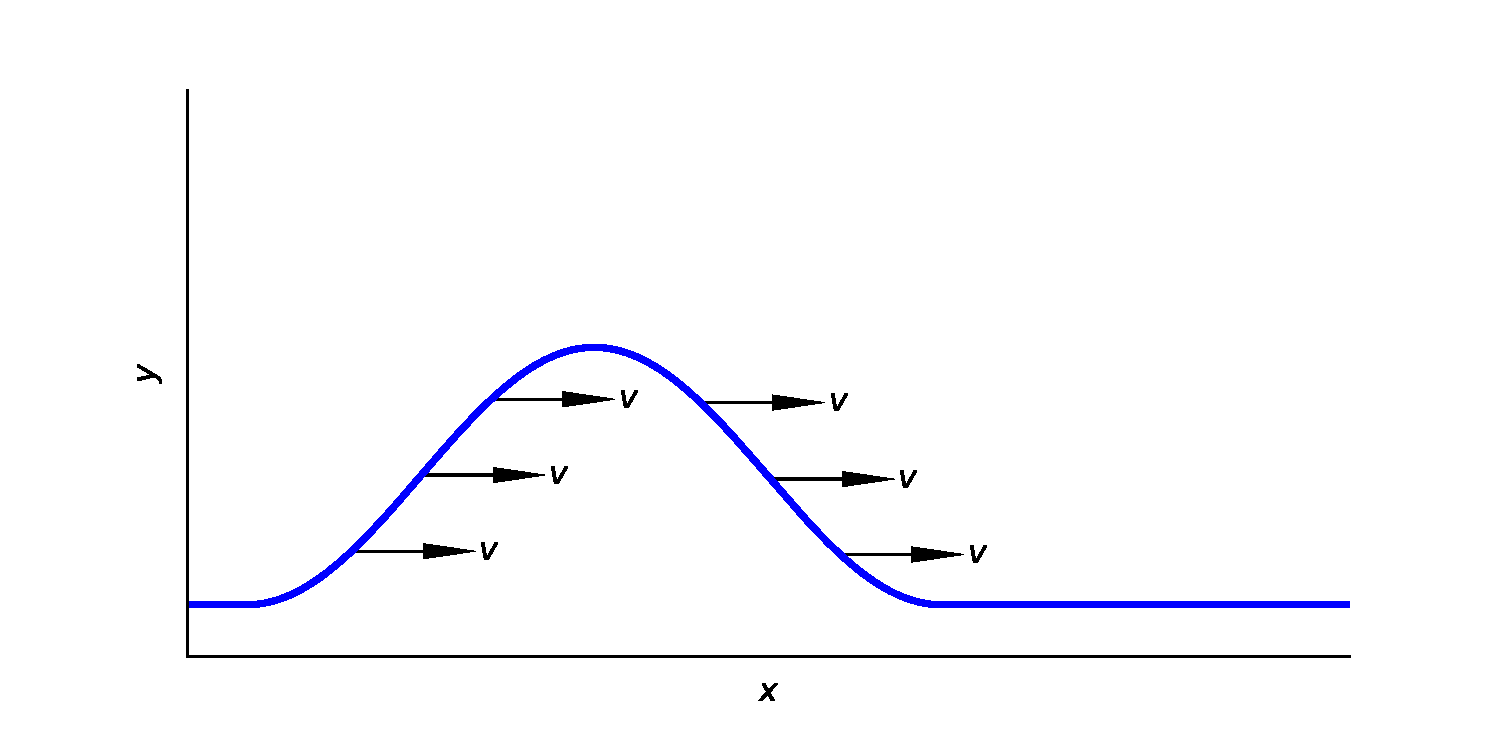
\includegraphics[width=0.7\linewidth]{visualisations/ch6-phasevelocity1} 

}

\caption{A reminder that every point in a wave pulse here moves at the same velocity $v$, such that the shape of the pulse is not changed.}\label{fig:ch6-phasevelocity1}
\end{figure}

For waves travelling on a string the phase velocity can be found from the tension in the string (\(F\)) and the linear mass density (mass per unit length) of the string (\(\mu\)):

\begin{equation}
v = \sqrt{\frac{F}{\mu}}
\end{equation}

This has parallels for soundwaves in a fluid, with phase velocity found from the bulk modulus \(B\) (a factor describing the fluid's resistance to compression) and the equilibrium density \(\rho\) of the fluid:

\begin{equation}
v_s = \sqrt{\frac{B}{\rho}}
\end{equation}

We can go further to look at the propatgation of sound waves in an isotropic solid (solid of constant composition) - however we can only use this to consider a thin section, not a bulk solid (this is an acceptable model for considering earth tremors in the Earth's crust). This time the phase velocity depends on the density of the solid \(\rho\) and either the Young's modulus (\(Y\), for longitudinal P waves) or the shear modulus (\(G\), for transverse S waves):

\begin{equation}
v_s = \sqrt{\frac{Y}{\rho}} \textrm{or} \sqrt{\frac{G}{\rho}}
\end{equation}

These equations descrie how wave phase velocities can be determined in solids and liquids; in a gas, we need to use other parameters, however the core relationship is still familiar:

\begin{equation}
v_s = \sqrt{\frac{\gamma RT}{M}} =  \sqrt{\frac{\gamma k_{\mathrm{B}}T}{m}}
\end{equation}

Here, the terms \(R\), \(T\) and \(M\) refer to the gas constant (units J K\textsuperscript{-1} mol\textsuperscript{-1}), absolute temperature (units K) and the molar mass of the gas (units kg mol\textsuperscript{-1}) respectively\footnote{Note that the molar mass is expressed in kg mol\textsuperscript{-1} here, rather than the more common g mol\textsuperscript{-1} ; the reason for this is to ensure continuity and present everything in SI units.}, while \(k_{\textrm{B}}\) and \(m\) refer to the Boltzmann constant (units J K\textsuperscript{-1}) and the mass of an individual gas molecule (units kg).

Finally, we can obtain a similar expression for the phase velocity of light waves:

\begin{equation}
c = \sqrt{\frac{1}{\mu_0 \epsilon_0}}
\end{equation}

\ldots where \mu\_0 and \epsilon\_0 are the permeability of free space and the permittivity of free space respectively.

\hypertarget{sec:ch6-summary}{%
\section{Summary}\label{sec:ch6-summary}}

In this chapter, we have introduced the principle of waves and the wave equation. Waves carry energy and momentum through space by localised organised oscillations without net transport of matter. They can be transverse (oscillation perpendicular to direction of propagation) or longitudinal (oscillation parallel to direction of propagation), or can have a more complex displacement pattern. Waves do not have to be sinusoidal, and can have any shape.

Any travelling wave can be described by the function in the form of \(y = f(x \pm vt)\) which satisfies the wave equation, relating the displacement of the medium (\(y\)) to the position of the wave (\(x\)) and the phase velocity (\(v\)).

\begin{equation}
\frac{\partial^2 y}{\partial x^2} = \frac{1}{v^2} \frac{\partial^2 y}{\partial t^2}
\end{equation}

Remember that the phase velocitycannot be predicted from the wave equation, but depends on the physics of the system. It generally results from a consideration of the elastic and inertial properties of the system. For waves on a string, \(v = \sqrt{\frac{F}{\mu}}\), where \(F\) is the tension in the string and \(\mu\) is the mass per unit length (linear mass density).

\hypertarget{sec:ch7-harmonicwaves}{%
\chapter{Harmonic Waves}\label{sec:ch7-harmonicwaves}}

\emph{Textbook link: Tipler and Mosca, Section 15.2}

A \emph{harmonic wave} is a general term for a wave which, at some instant of time, can be described by a sinusoidal function (\emph{i.e.} it is a sine or a cosine function). They are the simplest of waves to consider, and we will devote this chapter to exploring their properties.

\hypertarget{sec:ch7-sinecosine}{%
\section{Transverse sine and cosine waves}\label{sec:ch7-sinecosine}}

If we consider a string which is excited by a tuning fork or other object undergoing simple harmonic motion (SHM), we can imagine the shape of the save on the string at some instant of time appearing as a sine or a cosine wave (depending on our choice of origin) (Figure \ref{fig:ch7-transversesine1}):

\begin{figure}

{\centering 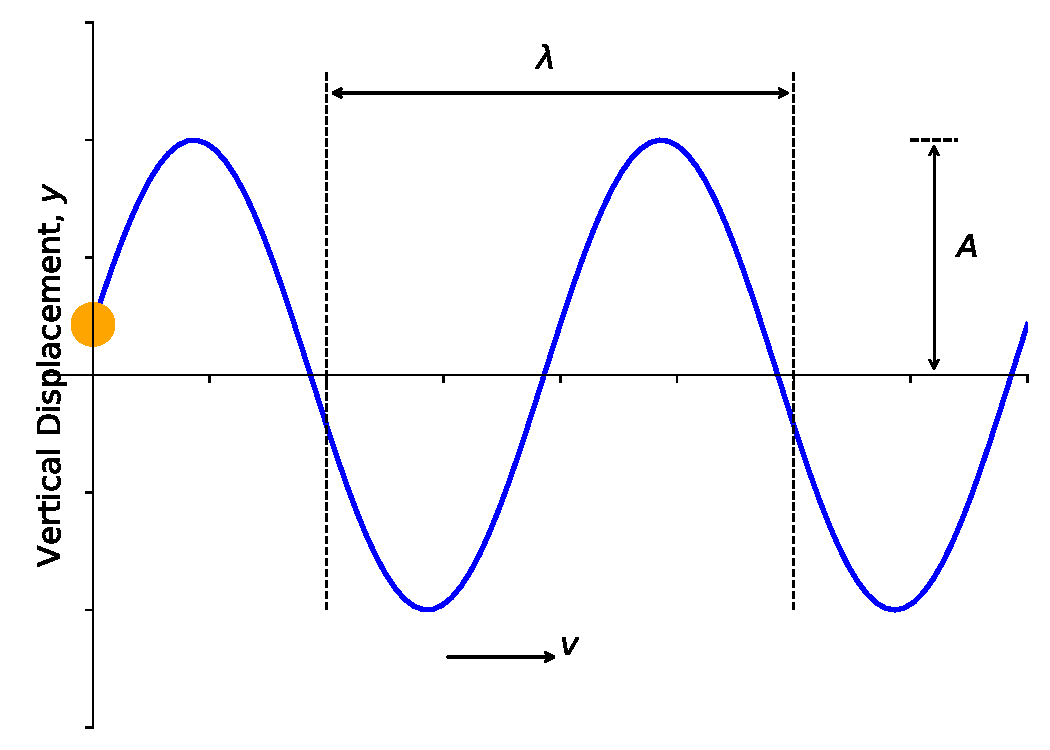
\includegraphics[width=0.7\linewidth]{visualisations/ch7-transversesine1} 

}

\caption{A sine wave in a string created by an oscillating particle.  The wavelength $\lambda$ is shown for one complete cycle, while the amplitude $A$ is defined as the maximum deviation from the origin point.}\label{fig:ch7-transversesine1}
\end{figure}

This sinusoidal appearance is known as a \textbf{harmonic wave}. Each point on the string oscillates up and down with the same frequency as the driving frequency. During the period \(T\), the wave moves through distance \(\lambda\):

\begin{equation}
v = \frac{\lambda}{T} = f\lambda
\label{eq:ch7-tranversesine1}
\end{equation}

\ldots where \(v\) is the phase velocity of the wave and \(f\) is the frequency in hertz (Hz), and \(\lambda\) defined as the \textbf{wavelength} \emph{i.e.} the spacial repeat distance of the wave.

A harmonic wave has a unique frequency and wavelength, and other waves (\emph{e.g.} wave pulses) may be regarded as a superposition of many harmonic waves of different frequencies (we will discuss the Fourier analysis of this later).

At any instant in time, the wave can be described by the relation in Equation \eqref{eq:ch7-tranversesine2}:

\begin{equation}
y = A \sin(kx + \delta)
\label{eq:tranversesine2}
\end{equation}

\ldots where \(A\) is the amplitude of the wave and \(\delta\) is the phase constant. Let's now choose the origin so that \(\delta\) is equal to zero (\emph{i.e.} there is no phase constant). Now we can show the periodic condition in Equation \eqref{eq:ch7-tranversesine3}:

\begin{equation}
\sin kx = \sin k(x+\lambda)
\label{eq:ch7-tranversesine3}
\end{equation}

Here we specify the periodic condition; the amplitude (and phase!) at position \(x\) is equal to the amplitude (and phase!) at position \(x\) \textbf{plus one wavelength}. Because this is a sine function, we know that, in order to achieve this condition, the value \(k\lambda\) must be equal to \(2\pi\):

\begin{equation}
\begin{array}{rcl}
\sin \theta &=& \sin \left( \theta + 2\pi \right)\\
\sin kx &=& \sin \left( kx + k\lambda\right) = \sin \left( kx + 2\pi \right) \\
k\lambda &=& 2\pi
\end{array}
\label{eq:ch7-tranvsersesine3b}
\end{equation}

This allows us to give a value for \(k\) (Equation \eqref{eq:ch7-tranversesine4}):

\begin{equation}
k = \frac{2\pi}{\lambda}
\label{eq:ch7-tranversesine4}
\end{equation}

The parameter \(k\) is defined as the \textbf{wave number} of the wave, in units radians per metre (rad m\textsuperscript{-1}).

\hypertarget{sec:ch7-travellingwaves}{%
\section{Travelling waves}\label{sec:ch7-travellingwaves}}

The wave we showed in Section \ref{sec:ch7-sinecosine} was a snapshot in time, so the wave was, in effect, static. We instead wish to consider a travelling wave. To do this, instead of writing \(x\) as in Equation \eqref{eq:tranversesine2} with \(x - vt\) (see Section \ref{sec:ch6-wavepulses}). Equation \eqref{eq:tranversesine2} then becomes Equation \eqref{eq:tranversesine5}:

\begin{equation}
y = A \sin k(x - vt) = A \sin (kx - kvt)
\label{eq:tranversesine5}
\end{equation}

As we have described, \(T\) is the period of the wave, so any point on the wave will oscillate up and down also with period \(T\). This means that, for the wave position at time \(t\), it will return to the same state at time \((t+T)\). We can therefore write Equation \eqref{eq:tranversesine5} in terms of this period:

\begin{equation}
\begin{array}{rcl}
y = A \sin \left( kx - kvt \right) &=& A \sin \left( kx - kv(t+T) \right) \\
&=& A \sin \left( kx - kvt - kvT \right)
\end{array}
\label{eq:ch7-travelling2}
\end{equation}

Applying the same reasoning as shown in Equation scheme \eqref{eq:ch7-tranvsersesine3b}, we are led to the result:

\begin{equation}
kvT = 2\pi
\end{equation}

If we revisit our discussions on SHM (Chapter \ref{sec:shm-freq-angularfreq}) we defined the relationship between \(T\) and \(2\pi\) (Equation \eqref{eq:ch1-definingomega1}) as \(T = \frac{2\pi}{\omega}\) (and also \(\omega = 2\pi f\)). This allows us to define a number of factors as follows:

\begin{itemize}
\tightlist
\item
  \textbf{Phase velocity}:
\end{itemize}

\begin{equation}
v = \frac{2\pi}{kT} = \frac{\omega}{k}
\label{eq:ch7-phasevel1}
\end{equation}

\begin{itemize}
\tightlist
\item
  \textbf{Travelling wave to the right}:
\end{itemize}

\begin{equation}
y = A \sin \left( kx - kvt \right) = A \sin \left( kx - \omega t \right)
\label{eq:ch7-travellingtoright1}
\end{equation}

\begin{itemize}
\tightlist
\item
  \textbf{Travelling wave to the left}:
\end{itemize}

\begin{equation}
y = A \sin \left( kx + kvt \right) = A \sin \left( kx + \omega t \right)
\label{eq:ch7-travellingtoleft1}
\end{equation}

It is worth noting for each of these factors:

\begin{enumerate}
\def\labelenumi{\arabic{enumi}.}
\tightlist
\item
  The sign of \(\omega\):

  \begin{itemize}
  \tightlist
  \item
    negative for waves travelling to right;
  \item
    positive for waves travelling to left
  \end{itemize}
\item
  The wave expressions can be shown to satisfy the wave equation by substitution.
\end{enumerate}

\hypertarget{sec:ch7-complexrep}{%
\section{Complex representation of waves}\label{sec:ch7-complexrep}}

We introduced complex numbers for descriptions of oscillations; we can use the same treatment for our wave equations. Just as \(\sin(kx - \omega t)\) and \(\cos(kx-\omega t)\) satisfy the wave equation, so too will \(\mathrm{e}^{\mathrm{i}(kx-\omega t)}\). It is often convenient to write the wave expression in a complex form as shown in Equation \eqref{eq:ch7-wavecomplex1}:

\begin{equation}
y = A \mathrm{e}^{\mathrm{i}(kx-\omega t)}
\label{eq:ch7-wavecomplex1}
\end{equation}

In this expression, the sine wave is given by the `imaginary' component of \(y\), while the cosine part is given by the `real' component.

\hypertarget{sec:ch7-energywavesstring}{%
\section{Energy carried by waves on a string}\label{sec:ch7-energywavesstring}}

Suppose we now have a string attached to an oscillating driver at one end. As the driver oscillates, it imparts energy to the string at \(x=0\) by:

\begin{enumerate}
\def\labelenumi{\arabic{enumi}.}
\tightlist
\item
  Stretching the string to give it potential energy, and
\item
  imparting transverse speed to the string to increase its kinetic energy.
\end{enumerate}

As the waves move along the string, so the energy is transported along the string.

\hypertarget{sec:ch7-peofstringsegment}{%
\subsection{Potential energy of string segment}\label{sec:ch7-peofstringsegment}}

We now consider the same string segment as we showed in Figure \ref{fig:ch6-waveeqnderiv1}, but now we consider it stretched (Figure \ref{fig:ch7-stretchedsegment1}). We can picture this as the string is ``relaxed'' in its `horizontal' orientation (length of segment is \(\Delta x\)), but when a wave passes along it, the string elongates to accommodate the curve of the wave form. This means our segment now takes on a new length \(\Delta l\).

\begin{figure}

{\centering 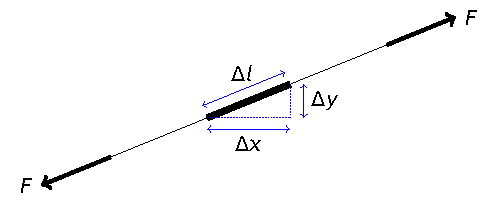
\includegraphics[width=0.7\linewidth]{visualisations/LaTeX/ch7-peofstringsegment} 

}

\caption{As the wave passes along a stretched string, we can consider it to be 'stretched'; considering a string element of lencth $\Delta x$, it is stretched to new length $\Delta l$ as the wave passes by.}\label{fig:ch7-stretchedsegment1}
\end{figure}

The work done (\Delta U) in stretching the segment \(\Delta x\) can be expressed as:

\begin{equation}
\Delta u = F(\Delta l - \Delta x)
\label{eq:ch7-workdonestring1}
\end{equation}

\ldots where \(F\) is the tension in the string and the extension is given by \((\Delta l - \Delta x)\). We can apply Pythagoras to relate \(\Delta x\) and \(\Delta l\):

\begin{equation}
\begin{array}{rcl}
\Delta l^2 &=& \Delta x^2 + \Delta y^2 \\
&=& \Delta x^2 \left[ 1 + \left( \dfrac{\Delta y}{\Delta x}\right)^2 \right]
\end{array}
\end{equation}

Therefore we can isolate \(\Delta l\):

\begin{equation}
\Delta l = \Delta x \left[ 1 + \left( \dfrac{\Delta y}{\Delta x}\right)^2 \right]^{\frac{1}{2}}
\end{equation}

We can approximate this expression by using the Taylor series expansion for \(\sqrt{1+n}\), where \(n = \left( \dfrac{\Delta y}{\Delta x}\right)^2\); assuming that the fraction is significantly less than one we can write this as an approximation and disregard terms past the first two terms:\footnote{The Taylor expansion for this expression is \(\sqrt{1+n} = 1+ \frac{n}{2} - \frac{n^2}{8} + \frac{n^3}{16} - \cdots\)}

\begin{equation}
\Delta l \approx \delta x \left[ 1 + \frac{1}{2}\left( \dfrac{\Delta y}{\Delta x}\right)^2 + \cdots \right]
\end{equation}

Rearranging this expression to obtain the expression for the extension of the string \(\Delta l - \Delta x\):

\begin{equation}
\Delta l - \delta x \approx   + \frac{\delta x}{2} \left( \dfrac{\Delta y}{\Delta x}\right)^2 + \cdots
\end{equation}

This now allows us to obtain an expression for the work done in stretching the spring solely in terms of the \(x\) and \(y\) displacement (from Equation \eqref{eq:ch7-workdonestring1})

\begin{equation}
\Delta u = \frac{F\Delta x}{2} \left( \dfrac{\Delta y}{\Delta x}\right)^2
\end{equation}

As we have an expression for \(y\) in terms of \(x\) (Equation \eqref{eq:tranversesine2}), we can differentiate this with respect to \(x\) to approximate \(\frac{\Delta y}{\Delta x}\):

\begin{equation}
\frac{\Delta y}{\Delta x} \simeq \frac{\mathrm{d} y}{\mathrm{d} x} = kA \cos (kx - \omega t)
\end{equation}

We also know that \(v^2 = \frac{F}{\mu}\) (from the wave equation), and that \(v = \frac{\omega}{k}\) (Equation \eqref{eq:ch7-phasevel1}), therefore:

\begin{equation}
\Delta U = \frac{1}{2} \left( \frac{\mu \omega^2}{k^2} \right) \Delta x \left( kA \cos (kx - \omega t) \right)^2
\end{equation}

Tidying up and cancelling, we obtain the expresion for the potential energy stored in an element of string of length \(\Delta x\) (Equation \eqref{eq:ch7-pestoredstring1}):

\begin{equation}
\Delta U = \frac{1}{2} \mu \omega^2 A^2 \Delta x \cos^2(kx-\omega t)
\label{eq:ch7-pestoredstring1}
\end{equation}

\hypertarget{sec:ch7-keofstringsegment}{%
\subsection{Kinetic energy of string segment}\label{sec:ch7-keofstringsegment}}

We will again consider the segment of string discussed in Section \ref{sec:ch7-peofstringsegment}; an element \(\Delta x\) of the string, of mass \(\Delta m\) (Figure \ref{fig:ch7-kestringsegment}).

\begin{figure}

{\centering 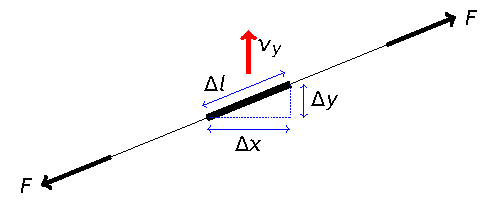
\includegraphics[width=0.7\linewidth]{visualisations/LaTeX/ch7-keofstringsegment} 

}

\caption{Similar to the situation shown above, the same string segment will have a kinetic energy associated with its velocity $v_y$.}\label{fig:ch7-kestringsegment}
\end{figure}

As before, the segment is stretched to new length \(\Delta l\), but the mass is still given by:

\begin{equation}
\Delta m = \mu \Delta x
\end{equation}

\ldots where \(\mu\) is the mass per unit length. We now use the \textbf{transverse velocity} of the segment (\emph{i.e.} \textbf{not} the wave velocity) to determine the kinetic energy of the segment:

\begin{equation}
\Delta KE = \frac{1}{2} \Delta m v_y^2 = \frac{1}{2} \mu \Delta x \left( \frac{\mathrm{d}y}{\mathrm{d}t} \right)^2
\end{equation}

Again, we know the expression for the vertical displacement \(y\) in terms of \(x\) and \(t\) (Equation \eqref{eq:tranversesine2}), so we now differentiate with respect to \(t\):

\begin{itemize}
\tightlist
\item
  \(y = A \sin(kx - \omega t)\)
\item
  \(v_y = \frac{\mathrm{d}y}{\mathrm{d}t} = -\omega A \cos(kx - \omega t)\)
\end{itemize}

Therefore our expression for the kinetic energy becomes:

\begin{equation}
\Delta KE =  \frac{1}{2} \mu \omega^2  A^2 \Delta x  \cos^2(kx - \omega t)
\label{eq:ch7-kestoredstring1}
\end{equation}

A quick comparison of Equations \eqref{eq:ch7-pestoredstring1} and \eqref{eq:ch7-kestoredstring1} shows that these expressions are identical; \emph{i.e.} the KE stored in the string is the \textbf{same} as the PE stored in the spring.

\hypertarget{sec:ch7-totenergystringsegment}{%
\subsection{Total energy of wave on a string}\label{sec:ch7-totenergystringsegment}}

We can therefore find the total energy of the string segment carrying a harmonic wave as the total of the kinetic and potential energies:

\begin{equation}
\Delta E = \Delta KE + \Delta U
\end{equation}

\emph{i.e.}:

\begin{equation}
\Delta E = \mu \omega^2  A^2 \Delta x  \cos^2(kx - \omega t)
\label{eq:ch7-totalenergywavestring1}
\end{equation}

Note that the energy of the segment varies with time with twice the frequency of the wave (since \(\cos^2 \theta = \frac{1}{2}(1+ \cos 2\theta)\)).

We can also define the average energy at any point (Equation \eqref{eq:ch7-averageenergystring1}) using the time-average definition \(\left< \cos^2 \theta \right> = \frac{1}{2}\):

\begin{equation}
\Delta E_{\mathrm{av}} = \frac{1}{2}\mu \omega^2 A^2 \Delta x
\label{eq:ch7-averageenergystring1}
\end{equation}

\ldots and we can define the average \emph{energy density} (per unit length) as:

\begin{equation}
\varepsilon = \frac{\Delta E_{\mathrm{av}}}{\Delta x} = \frac{1}{2} \mu \omega^2 A^2
\end{equation}

There are several things to note from this derivation:

\begin{itemize}
\tightlist
\item
  KE is at a maximum when displacement is zero
\item
  At this point the string is most stretched, so PE is at a maximum also
\item
  PE and KE are \textbf{in phase} (unlike in a pendulum)
\end{itemize}

These points are illustrated in Figure \ref{fig:ch7-kepestringplot1}.

\begin{figure}

{\centering 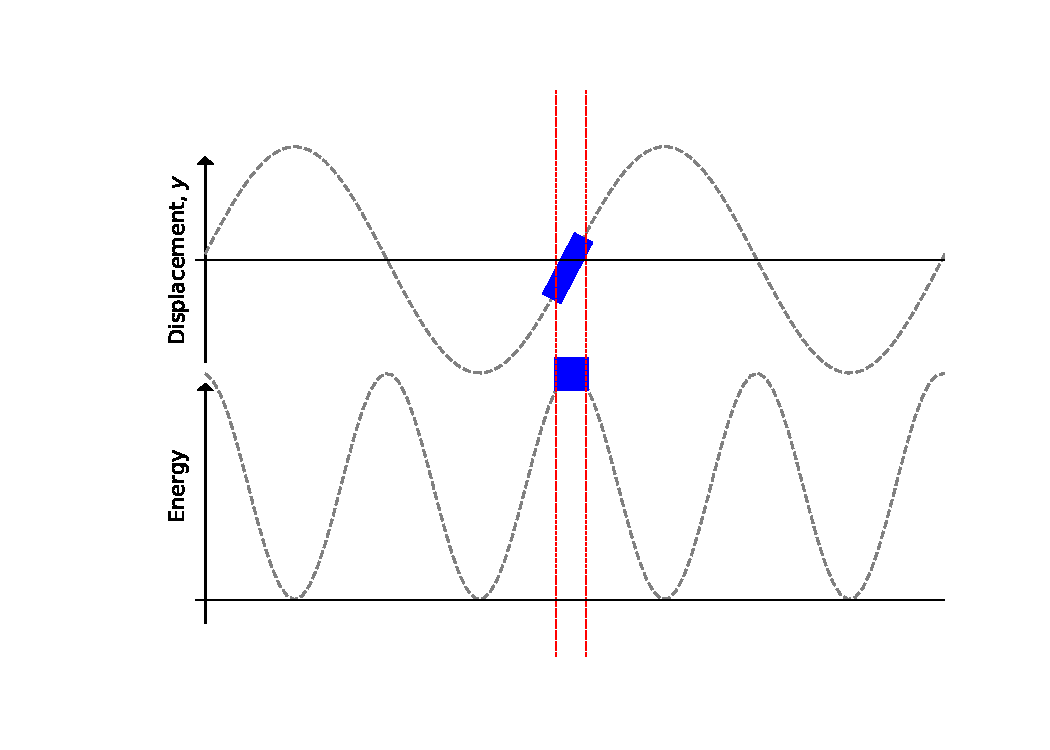
\includegraphics[width=0.7\linewidth]{visualisations/ch7-kepestringplot1} 

}

\caption{The kinetic energy and potential energy of a displaced string element have maxima and minima at the same points in the oscillation; as the element passes through the origin (top plot), it is at its most stretched (PE maximum), and it is traveling at its fastest (KE maximum).}\label{fig:ch7-kepestringplot1}
\end{figure}

\hypertarget{sec:ch7-transportenergypower}{%
\subsection{Transport of energy and power}\label{sec:ch7-transportenergypower}}

As the wave propagates along the string, energy is transported by the moving wavefront at speed \(v\). The average energy passing a point on the string in time \(\Delta t\) is the average energy in the segment of length \(\Delta x = v\Delta t\). This means we can rewrite Equation \eqref{eq:ch7-averageenergystring1}:

\begin{equation}
\Delta E_{\mathrm{av}} = \frac{1}{2}\mu \omega^2 A^2 v \Delta t
\label{eq:ch7-averageenergystring2}
\end{equation}

Since the power transmitted is a \emph{rate of change of energy}, \emph{i.e.} \(\frac{\Delta E}{\Delta t}\), we can obtain an expression for the average power transmitted:

\begin{equation}
\Delta P_{\mathrm{av}} = \frac{\mathrm{d} E_{\mathrm{av}}}{\mathrm{d}t} \approx \frac{\Delta E_{\mathrm{av}}}{\Delta t} = \frac{1}{2}\mu \omega^2 A^2 v
\label{eq:ch7-averagepowerstring1}
\end{equation}

From this result, we can see that both the average energy and average power transmitted are both proportional to \(A^2\); a similar observation as in SHM (Chapter \ref{sec:shm}).

\hypertarget{sec:ch7-summary}{%
\section{Summary}\label{sec:ch7-summary}}

We have covered a large amount of derivations in this chapter, however the takehome points are the following:

When describing sine waves travelling through a medium, the following statements apply:

\begin{itemize}
\tightlist
\item
  For a wave travelling to the \textbf{right}: \(y = A\sin(kx-\omega t)\)
\item
  For a wave travelling to the \textbf{left}: \(y = A\sin(kx+\omega t)\)
\item
  The \textbf{phase velocity}: \(v = \frac{\omega}{k}\) m s\textsuperscript{-1}
\end{itemize}

\ldots where:

\begin{itemize}
\tightlist
\item
  \(k\) = wavenumber = \(\frac{2\pi}{\lambda}\)
\item
  \(\lambda\) = wavelength /m
\item
  \(\omega\) = angular frequency = \(2\pi f\) /rad m\textsuperscript{-1}
\item
  \(f\) = frequency /Hz = \(\frac{1}{T}\)
\item
  \(T\) = period /s
\item
  \(A\) = amplitude /m
\end{itemize}

The average energy carried by a wave (per unit length) is given by:

\begin{equation}
\varepsilon = \frac{\Delta E_{\mathrm{av}}}{\Delta x} = \frac{1}{2} \mu \omega^2 A^2
\end{equation}

\ldots and the average power transmitted by the wave is given by:

\begin{equation}
\Delta P_{\mathrm{av}} = \frac{\Delta E_{\mathrm{av}}}{\Delta t} = \frac{1}{2}\mu \omega^2 A^2 v
\end{equation}

\hypertarget{sec:ch8-reflectiontrans}{%
\chapter{Reflection and Transmission at boundaries}\label{sec:ch8-reflectiontrans}}

We now turn our attention to what happens to waves and wave pulses when they encounter boundaries. We define a boundary as the dividing line between regions with different phase velocity. In the context of imagining our waves moving along strings, a boundary can exist either between the string and a rigid anchoring point, or at a point where the two strings join, each with a different mass density (\emph{i.e.} a thick string joining to a thin string).

\textbf{Any} wave incident on such a boundary between regions with different phase velocities will be partly reflected back from the boundary and partly transmitted through the boundary.

In the case of a boundary between a thick string and a thin string, the phase velocity \(v\) is related to the tension \(F\) and the mass density \(\mu\) \emph{via} \(v^2 = \frac{F}{\mu}\); \emph{i.e.} heavier strings will have a lower phase velocity.

Considering reflection/transmission across such a boundary in a purely qualitative manner:

\begin{enumerate}
\def\labelenumi{\arabic{enumi}.}
\tightlist
\item
  A wave propagating along a thin string towards a boundary with a thicker string will be reflected from the boundary \textbf{with inversion}, as well as a proportion of the energy transmitted as a wave into the thicker string.
\item
  A wave propagating along a thick string towards a boundary with a thinner string will be reflected from the boundary \textbf{without inversion}, as well as a proportion of the energy transmitted as a wave into the thinner string.
\end{enumerate}

This qualitative outcome is illustrated in Figures \ref{fig:ch8-thickthininversion1} and \ref{fig:ch8-thickthininversion1b}.

\begin{figure}

{\centering 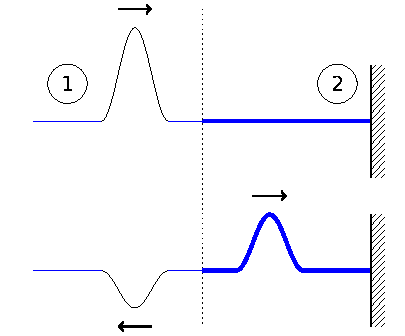
\includegraphics[width=0.7\linewidth]{visualisations/LaTeX/ch8-wavesonstrings1} 

}

\caption{When a wavepulse originates in string 1 (where $\mu_1 \ll \mu_2$), the wave will be both reflected with inversion and partially transmitted into string 2 of greater $\mu$}\label{fig:ch8-thickthininversion1}
\end{figure}

\begin{figure}

{\centering 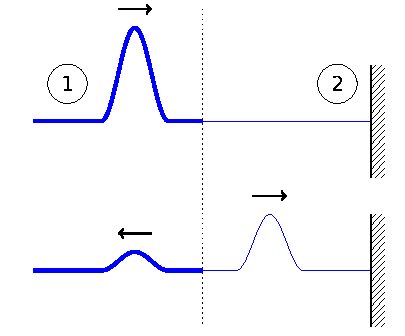
\includegraphics[width=0.7\linewidth]{visualisations/LaTeX/ch8-wavesonstrings2} 

}

\caption{If we reverse the situation with the wavepulse originating in the string with greater $\mu$ (now $\mu_1 \gg \mu_2$), the wave is still partially transmitted into string 2, but the reflection within string 1 is no longer inverted.}\label{fig:ch8-thickthininversion1b}
\end{figure}

If instead we fix a uniform string to an immovable anchor rather than another, thicker, string, we will get complete reflection of the wave pulse with inversion. This is akin to saying the anchor has an infinite mass density, \(\mu\).

To quantitatively assess these outcomes, we can obtain the reflected and transmitted amplitudes for harmonic waves by considering the power transmitted through the string as the wave propagates.

\hypertarget{sec:ch8-powertransmittedreflected}{%
\section{Power transmitted and reflected at a boundary}\label{sec:ch8-powertransmittedreflected}}

The principles of energy conversion state that, as a wave encounters a boundary, the energy in the incident wave must equal the total energy of the reflected and transmitted waves. This principle therefore also applies to the total power of the system, \emph{i.e.}:

\begin{equation}
P_i = P_r + P_t
\label{eq:ch8-powerconservation1}
\end{equation}

We can therefore use Equation \eqref{eq:ch7-averagepowerstring1} to derive an expression for the power before and the powers after the wave encounters the boundary (Equation \eqref{eq:ch8-powerconservation2}):

\begin{equation}
\frac{1}{2}\mu_1 \omega^2 A_i^2 v_1 = \frac{1}{2}\mu_1 \omega^2 A_r^2 v_1 + \frac{1}{2}\mu_2 \omega^2 A_t^2 v_2
\label{eq:ch8-powerconservation2}
\end{equation}

\ldots or, since \(\omega = v_n k_n\) and \(F = \mu_n v_n^2\) (rearrangments of equations seen previously):

\begin{equation}
\frac{1}{2} F k_1 \omega A_i^2  = \frac{1}{2}F k_1 \omega A_r^2 + \frac{1}{2}F k_2 \omega A_t^2
\label{eq:ch8-powerconservation3}
\end{equation}

Note that:
* \(A_i\), \(A_r\) and \(A_t\) are the amplitudes of the incident, reflected and transmitted waves respectively;
* \(\mu_1\), \(v_1\), \(\mu_2\), \(v_2\) refer to the mass per unit length and the phase velocities for strings 1 and 2 respectively;
* \(k_1\) and \(k_2\) are the wavenumbers for each of the two strings;
* \(\omega\) is the \textbf{same} for all waves - this depends only on the source;
* \(\lambda\) will be \textbf{different} on each string; since \(\lambda = \frac{v}{f} = \frac{2\pi v}{\omega}\), \emph{i.e.} \(\lambda\) will be smaller on the heavier string;
* Conversely \(k = \frac{2\pi}{\lambda}\) will be larger on the heavier string;
* \(\mu = \frac{F}{v^2}\); the tension \(F\) will be the same in both strings.

When we compare the proportion of the incident power which is reflected, we can show that:

\begin{equation}
\frac{\textrm{Reflected power}}{\textrm{Incident power}} = \frac{k_1 A_r^2}{k_1 A_i^2} = \left( \frac{k_1 - k_2}{k_1 + k_2} \right)^2
\label{eq:ch8-powerratio1}
\end{equation}

We can also show the proportion of the incident power which is transmitted:

\begin{equation}
\frac{\textrm{Transmitted power}}{\textrm{Incident power}} = \frac{k_2 A_t^2}{k_1 A_i^2} =  \frac{4k_1 k_2}{\left( k_1 + k_2\right)^2}
\label{eq:ch8-powerratio2}
\end{equation}

\textbf{Note} These results \textbf{only} hold for waves on strings where the tension, \(F\), is the same in both strings. We will discuss a more general result in the next section.

\hypertarget{proof-of-power-ratios}{%
\subsection*{Proof of power ratios}\label{proof-of-power-ratios}}
\addcontentsline{toc}{subsection}{Proof of power ratios}

From our expression of the conservation of powers (Equation \eqref{eq:ch8-powerconservation3}), we can cancel the common terms:

\begin{equation}
k_1  A_i^2  =  k_1  A_r^2 +  k_2  A_t^2
\label{eq:ch8-powerratio1b}
\end{equation}

However, at the interface, the wave must be continuous on both sides; therefore the amplitude on each side must be the same:

\begin{equation}
A_i + A_r  =  A_t
\label{eq:ch8-powerratio1c}
\end{equation}

We now substitute Equation \eqref{eq:ch8-powerratio1c} into \eqref{eq:ch8-powerratio1b} to eliminate \(A_r\):

\begin{equation}
k_1  A_i^2  =  k_1  (A_t - A_i)^2 +  k_2  A_t^2
\label{eq:ch8-powerratio1d}
\end{equation}

We can then expand and rearrange this:

\begin{equation}
\begin{array}{rcl}
k_1  A_i^2  &=&  k_1  (A_t - A_i)^2 +  k_2  A_t^2\\
            &=& k_1 (A_t^2 - 2A_t A_i + A_i^2) + k_2  A_t^2 \\
    0       &=& k_1 A_t^2 - 2 k_1 A_t A_i + k_2  A_t^2 \\
            &=& k_1\dfrac{A_t^2}{A_i^2} - 2 k_1 \dfrac{A_t}{A_i} + k_2 \dfrac{A_t^2}{A_i^2} \\
    0       &=& \left(\dfrac{A_t}{A_i} \right)^2 (k_1 + k_2) - 2 k_1 \dfrac{A_t}{A_i} \\
\end{array}
\label{eq:ch8-powerratio1e}
\end{equation}

This is a quadratic equation, and we can then say the following; either:

\begin{equation}
\frac{A_t}{A_i} = 0
\end{equation}

\ldots which represents total reflection (zero transmission), and not what we would expect to have with two joined strings, or:

\begin{equation}
\left(\frac{A_t}{A_i}\right) = \frac{2k_1}{k_1 + k_2}
\end{equation}

\ldots from which we obtain:

\begin{equation}
\frac{k_2}{k_1} \left(\frac{A_t}{A_i}\right)^2 = \frac{4k_1 k_2}{(k_1 + k_2)^2}
\end{equation}

\ldots as required in Equation \eqref{eq:ch8-powerratio2} for the ratio of transmitted to incident power.

We can obtain the result for Equation \eqref{eq:ch8-powerratio1} for ratio of reflected to incident power in a similar manner by substitution of Equation \eqref{eq:ch8-powerratio1c} into \eqref{eq:ch8-powerratio1b} to instead eliminate \(A_t\).

\hypertarget{sec:ch8-examplereflectiontransmission}{%
\section{Example of reflection and transmission}\label{sec:ch8-examplereflectiontransmission}}

Consider a wave travelling from a light string to a heavy string, where \(\mu_2 = 4\mu_1\).

Remember that:
\begin{equation}
\mu = \frac{F}{v^2} = F\frac{k^2}{\omega^2}
\end{equation}

\emph{i.e.}
\begin{equation}
k \propto \sqrt{\mu}
\end{equation}

We can therefore determine:

\begin{itemize}
\tightlist
\item
  \(k_2 = 2 k_1\) via the square-root relationship
\item
  The fraction of power reflected will be:
  \begin{equation}
  \frac{A_r^2}{A_i^2} = \left( \frac{1-2}{1+2}\right)^2 = \frac{1}{9}
  \end{equation}
\item
  The fraction of power transmitted:
  \begin{equation}
  \frac{k_2 A_t^2}{k_1 A_i^2} = \left( \frac{4 \times 2 \times 1}{(1+2)^2}\right) = \frac{8}{9}
  \end{equation}
\end{itemize}

\hypertarget{sec:ch8-stringimpedeance}{%
\section{The impedance of a piece of string}\label{sec:ch8-stringimpedeance}}

The examples we considered in Secion \ref{sec:ch8-powertransmittedreflected} were a particular result under constant tension. We can generalise the result by considering the impedances of the media on either side of the boundary.

We discussed the concept of impedance (both electrical and mechanical) in Section \ref{sec:ch5-impedance}; however the salient points are:

\begin{itemize}
\tightlist
\item
  ``Impedance'' describes the property of a system which resists motion, either mechanical or motion of charge;
\item
  Any material through which waves propagate presents impedance to those waves;
\item
  In general, impedance depends on inertia and elasticity;
\item
  For a string, we define impedance as:
  \begin{equation}
  Z = \frac{\textrm{transverse force}}{\textrm{transverse velocity}}
  \end{equation}
  \emph{i.e.} for a given force, a large \(Z\) implies a small velocity and \emph{vice versa};
\item
  Similar definitions can be written for longitudinal waves.
\end{itemize}

We now consider a string which is driven by an oscillating force (Figure \ref{fig:ch8-impedencestring1})

\begin{figure}

{\centering 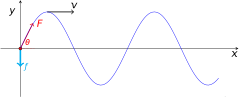
\includegraphics[width=0.7\linewidth]{visualisations/LaTeX/ch8-wavesonstrings3} 

}

\caption{When a wave is driven by an oscillating force at its origin ($f$), the element of the string indicated by the dot experiences the tension within the string, $F$, at angle $\theta$ from the direction of propagation.}\label{fig:ch8-impedencestring1}
\end{figure}

The driving force on this string is given by the relationship:

\begin{equation}
f = -f_0 \cos \omega t = -f_0 \mathrm{e}^{\mathrm{i}\omega t}
\end{equation}

This driving force is negative because \(f\) points downwards at time \(t = 0\).

As this is a wave, the vertical displacement at any point is given by the relationship:

\begin{equation}
y = A \mathrm{e}^{\mathrm{i}(kx - \omega t)}
\end{equation}

We now consider the tension in the string, \(F\), and resolve this in the transverse direction. At \(x = 0\), we assume small angle of \(\theta\):

\begin{equation}
\begin{array}{rcll}
f &=& -F\sin \theta \\
  &\simeq &  -F \tan \theta & \textsf{for small angles}\\
  &=& -F \dfrac{\partial y}{\partial x}
\end{array}
\end{equation}

We can now use the definition of impedance given above (\(Z = \frac{\textsf{force}}{\textsf{velocity}}\)) and the expressions for the force and velocity:

\begin{equation}
\begin{array}{rcl}
Z &=& \dfrac{f}{v_y} \\
 &=& -F\dfrac{\partial y}{\partial x} \div \dfrac{\partial y}{\partial t}
\end{array}
\end{equation}

We already have expressions for \(\frac{\partial y}{\partial x}\) and \(\frac{\partial y}{\partial t}\) by differentiating the wave equation \(y = A \mathrm{e}^{\mathrm{i}(kx - \omega t)}\):

\begin{equation}
\frac{\partial y}{\partial x} = ik A \mathrm{e}^{\mathrm{i}(kx - \omega t)}
\end{equation}

\begin{equation}
\frac{\partial y}{\partial t} = -i \omega A \mathrm{e}^{\mathrm{i}(kx - \omega t)}
\end{equation}

Therefore:

\begin{equation}
\begin{array}{rcl}
Z &=& \dfrac{-F \times ik A \mathrm{e}^{\mathrm{i}(kx - \omega t)}}{-i \omega A \mathrm{e}^{\mathrm{i}(kx - \omega t)}}\\
  &=& \dfrac{Fk}{\omega}
\end{array}
\end{equation}

Remember also that the phase velocity \(v = \frac{\omega}{k}\), so we can also express the impedance as \(Z = \frac{F}{v}\) and \(Z = \mu v\) (because \(v^2 = \frac{F}{\mu}\)), where \(\mu\) is the mass per unit length of the string and \(F\) is the tension within the string.

\hypertarget{sec:ch8-reflecttrans2}{%
\section{Reflection and transmission revisited}\label{sec:ch8-reflecttrans2}}

We can now express our previous result of the reflection and transmission coefficients (derived in Equation \eqref{eq:ch8-powerratio1e}) more generally:

Reflection coefficient:

\begin{equation}
\frac{A_r}{A_i} = \frac{Z_1 - Z_2}{Z_1 + Z_2}
\label{eq:ch8-reflectioncoeff1}
\end{equation}

Transmission coefficient:

\begin{equation}
\frac{A_t}{A_i} = \frac{2 Z_1 }{Z_1 + Z_2}
\label{eq:ch8-transmissioncoeff1}
\end{equation}

Writing these in terms of the power (the approach used in Section \ref{sec:ch8-powertransmittedreflected}), we obtain the following expressions:

\begin{equation}
\frac{\textsf{Reflected power}}{\textsf{Incident power}} = \frac{Z_1 A_r^2}{ Z_1 A_i^2} = \left(\frac{Z_1 - Z_2}{Z_1 + Z_2}\right)^2
\label{eq:ch8-reflectioncoeff2}
\end{equation}

and:

\begin{equation}
\frac{\textsf{Transmitted power}}{\textsf{Incident power}} = \frac{Z_2 A_t^2}{ Z_1 A_i^2} = \frac{4 Z_1 Z_2}{(Z_1 + Z_2)^2}
\label{eq:ch8-transmissioncoeff2}
\end{equation}

These are general expressions which apply in mechanical, electrical and optical systems. From them, we can see that:

\begin{itemize}
\tightlist
\item
  If \(Z_2 > Z_1\), the reflected wave is inverted;

  \begin{itemize}
  \tightlist
  \item
    From Equation \eqref{eq:ch8-reflectioncoeff1}, the term \(Z_1 - Z_2\) is negative under these conditions, leading to a negative amplitude
  \end{itemize}
\item
  If the second string is a ``wall'' (\emph{i.e.} immovable, infinite \(\mu\))

  \begin{itemize}
  \tightlist
  \item
    \(Z_2 \rightarrow \infty\);
  \item
    \(A_r = - A_i\) (by energy conservation);
  \item
    \(A_t = 0\);
  \item
    Therefore the wave is fully reflected and inverted.
  \end{itemize}
\item
  If \(Z_2 = Z_1\) we have:

  \begin{itemize}
  \tightlist
  \item
    Impedance matching;
  \item
    No reflection;
  \item
    Maximum power transfer.
  \end{itemize}
\end{itemize}

\hypertarget{sec:ch8-impedancemisccases}{%
\section{Impedance - Miscellaneous cases}\label{sec:ch8-impedancemisccases}}

For \textbf{longitudinal (sound) waves}, generally we expect the impedance \(Z\) to be described by \(Z = \rho_0 v_p\), where:

\begin{itemize}
\tightlist
\item
  \(\rho\) is the mean density of the medium
\item
  \(v_p\) is the phase velocity of the wave
\end{itemize}

Example values for longitudinal sound waves are:
* Air: \textasciitilde{} \(400\) kg m\textsuperscript{-2} s\textsuperscript{-1}
* Water: \(1.45 \times 10^6\) kg m\textsuperscript{-2} s\textsuperscript{-1}
* Steel: \(3.9 \times 10^7\) kg m\textsuperscript{-2} s\textsuperscript{-1}

For \textbf{transverse waves on a string}, the impedance \(Z\) is described by \(Z = \mu v_p\), where:

\begin{itemize}
\tightlist
\item
  \(\mu\) is the mass per unit length
\item
  \(v_p\) is the phase velocity of the wave
\end{itemize}

For \textbf{electromagnetic waves}, the impedance depends on the medium under consideration:

\begin{itemize}
\item
  In a dielectric medium:
  \begin{equation}
  Z = \sqrt{\frac{\mu \mu_0}{\epsilon \epsilon_0}}
  \end{equation}
  where in this case \(\mu\) and \(\epsilon\) are the permittivity and the permeability of the medium.
\item
  In free space:
  \begin{equation}
  Z = \sqrt{\frac{ \mu_0}{ \epsilon_0}} = 376.6 \Omega
  \end{equation}
\item
  For a light wave in a dielectric medium:
  \begin{equation}
  Z = \frac{1}{n}
  \end{equation}
  where \(n\) is the refractive index of the medium (see later).
\end{itemize}

\hypertarget{sec:ch9-sounddoppler}{%
\chapter{Sound waves and the Doppler effect}\label{sec:ch9-sounddoppler}}

\emph{Textbook link: Tipler and Mosca, Section 15.2-4}
As has been mentioned already, sound waves are a longitudinal wave propagated by the localised displacement of air molecules in the direction of propagation. This displacement of air molecules within sound waves can be described by the function shown in Equation\eqref{eq:ch9-soundwaveeq1}.

\begin{equation}
s(x,t) = s_0 \sin (kx - \omega t)
\label{eq:ch9-soundwaveeq1}
\end{equation}

In contrast to the transverse waves previously discussed, there are now only two dimensions to this function; while we considered the transverse displacement \(y\) of an element of the medium carrying the transverse wave, in this longitudinal wave the longitudinal displacement \(s\) is in the \(x\) direction, \emph{i.e.} the same direction as the propagation of the wave.

This displacement of the molecules leads to changes in both the density (\(\rho\)) and the pressure (\(p\)) of the medium. It is worth recognising that both \(p\) and \(\rho\) are out of phase with the displacement (when the displacement is at a maximum, the pressure and density are at a minimum):

\begin{equation}
p = p_0 \sin (kx - \omega t - \frac{\pi}{2})
\label{eq:ch9-soundwaveeq2}
\end{equation}

\ldots{} where the initial pressure \(p_0 = \rho \omega v s_0\) and \(v\) is the phase velocity.

\hypertarget{sec:ch9-energysoundwaves}{%
\section{Energy of sound waves}\label{sec:ch9-energysoundwaves}}

When considering the energy of sound waves, we can examine the expression we already have for transverse waves and adapt this for our longitudinal waves.

Recall that the expression for the energy within a transverse wave is given in Equation \eqref{eq:ch7-averageenergystring1}:

\begin{equation}
\Delta E_{\mathrm{av}} = \frac{1}{2}\mu \omega^2 A^2 \Delta x
\end{equation}

To adapt this for longitudinal sound waves, we perform the following substiutions:

\begin{itemize}
\tightlist
\item
  We replace the linear mass density \(\mu\) (units kg m\textsuperscript{-1}) with the density of the medium, \(\rho\) (units kg m\textsuperscript{-3})
\item
  We replace our transverse amplitude \(A\) with the longitudinal displacement \(s_0\)
\item
  To keep units congruent, we replace the change in segment length caused by the wave \(\Delta x\) with the change in segment volume caused by the wave \(\Delta V\)
\end{itemize}

Our result is therefore:

\begin{equation}
\Delta E_{\mathrm{av}} = \frac{1}{2}\rho \omega^2 s_0^2 \Delta V
\label{eq:ch9-averageenergysound1}
\end{equation}

\hypertarget{sec:ch9-waveintensity}{%
\section{Wave intensity}\label{sec:ch9-waveintensity}}

We have mentioned that with sound waves we are now considering a three-dimensional volume. This means we need to consider the effect of this on the energy of the wave at a distance \(r\) from its origin. The energy at a given distance will be spready uniformly over a spherical surface; therefore we need to consider the power per unit area of this surface. This is the \textbf{intensity} of the wave.

\begin{equation}
I = \frac{P_\text{av}}{4\pi r^2}
\label{eq:ch9-waveintensity1}
\end{equation}

We already know that the average power is defined as the rate of change of the average energy:

\begin{equation}
P_\text{av} = \frac{\Delta E_\text{av}}{\Delta t}
\end{equation}

We can therefore rewrite Equation \eqref{eq:ch9-waveintensity1} taking this into account.

\begin{equation}
\begin{array}{rcl}
I & = &  \dfrac{\Delta E_\text{av}}{4\pi r^2 \Delta r} \dfrac{\Delta r}{\Delta t} \\
 &=& \dfrac{\Delta E_\text{av}}{\Delta V} v
\end{array}
\label{eq:ch9-waveintensity2}
\end{equation}

In Equation \eqref{eq:ch9-waveintensity2} we idenitfy the term \(\frac{\Delta r}{\Delta t}\); this is the speed at which the wave travels from the centre of the sphere, so is the phase velocity \(v\). We can also say that the term \(4 \pi r^2 \Delta r\) is the rate of change of volume, \(\Delta V\). We now use our expression for the average energy (Equation \eqref{eq:ch9-averageenergysound1}) to simplify this expression:

\begin{equation}
I = \frac{1}{2}\rho \omega^2 s_0^2 v = \frac{p_0^2}{2\rho v}
\label{eq:ch9-waveintensity3}
\end{equation}

In other words, the intensity of the sound wave travelling at constant speed \(v\) through a medium of constant density \(\rho\) at a point in space is proportional to the square of the amplitude of the wave, \(p_0\).

\hypertarget{sec:ch9-intensitylevels}{%
\section{Levels of intensity}\label{sec:ch9-intensitylevels}}

The human ear perceives sounds according to the logarithm of their intensity - not the absolute value of the intensity.\footnote{When you encounter electronics you will find potentiometers labelled ``audio taper''; this describes their use in audio applications in which the resistance is a logarithmic response to accommodate our logarithmic perception of sound. } To represent an \textbf{intensity level} we use the term \textbf{decibel} (dB). This intensity level, \(\beta\) is represented in Equation \eqref{eq:ch9-decibel1} as follows:

\begin{equation}
\beta = 10 \log_{10}\left(\frac{I}{I_0}\right)
\label{eq:ch9-decibel1}
\end{equation}

The term \(I_0\) is the absolute intensity considered to be at the absolute limit of human hearing, where \(I_0 = 10^{-12}\) W m\textsuperscript{-2}. A description of approximate intensity levels is shown in Table \ref{tab:ch9-decibeldescription1}.

\begin{longtable}[]{@{}ll@{}}
\caption{\label{tab:ch9-decibeldescription1} A description of the approximate decibel level of particular sounds.}\tabularnewline
\toprule
\(\beta\) /dB & Description\tabularnewline
\midrule
\endfirsthead
\toprule
\(\beta\) /dB & Description\tabularnewline
\midrule
\endhead
0 & Hearing threshold\tabularnewline
40 & Library\tabularnewline
70 & Busy traffic\tabularnewline
120 & Pain threshold\tabularnewline
\bottomrule
\end{longtable}

\hypertarget{sec:ch9-dopplereffect1}{%
\section{The Doppler Effect (non-relativistic)}\label{sec:ch9-dopplereffect1}}

You have already met the Doppler effect for light in the context of the Special Relativity course; here we will briefly revisit it in the context of non-relativistic cases.

The general principles of the Doppler effect are unchanged, namely:

\begin{itemize}
\tightlist
\item
  If the source and observer move relative to each other, the observed frequency is different from the emitted frequency;
\item
  When the source and observer move towards each other, \(f_{\textsf{obs}} > f_{\textsf{source}}\);
\item
  When the source and observer move away from each other, \(f_{\textsf{obs}} < f_{\textsf{source}}\);
\item
  The frequency change, \(\Delta f\), depends on whether the source or observer move relative to each other.
\end{itemize}

Consider a source moving relative to its surrounding medium at a speed of \(u_s\). We can visualise this as a moving `dipper' in a pool of water (Figure \ref{fig:ch9-dopplerdipper1})

\begin{figure}

{\centering 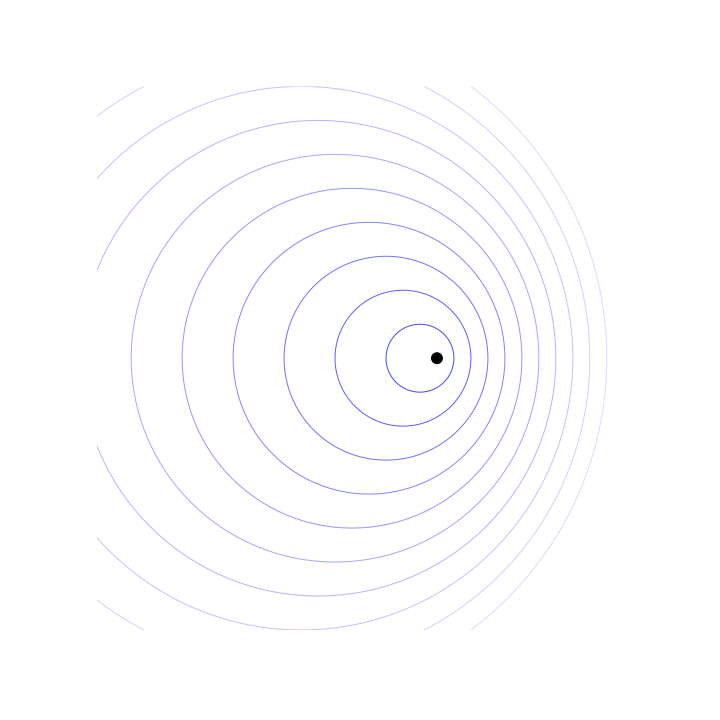
\includegraphics[width=0.7\linewidth]{visualisations/ch9-doppler1} 

}

\caption{When a dipper (marked by the black dot) moves relative to the water, we see that the wavefronts 'bunch' in the direction of motion and diverge behind the motion of the dipper.}\label{fig:ch9-dopplerdipper1}
\end{figure}

\begin{figure}

{\centering 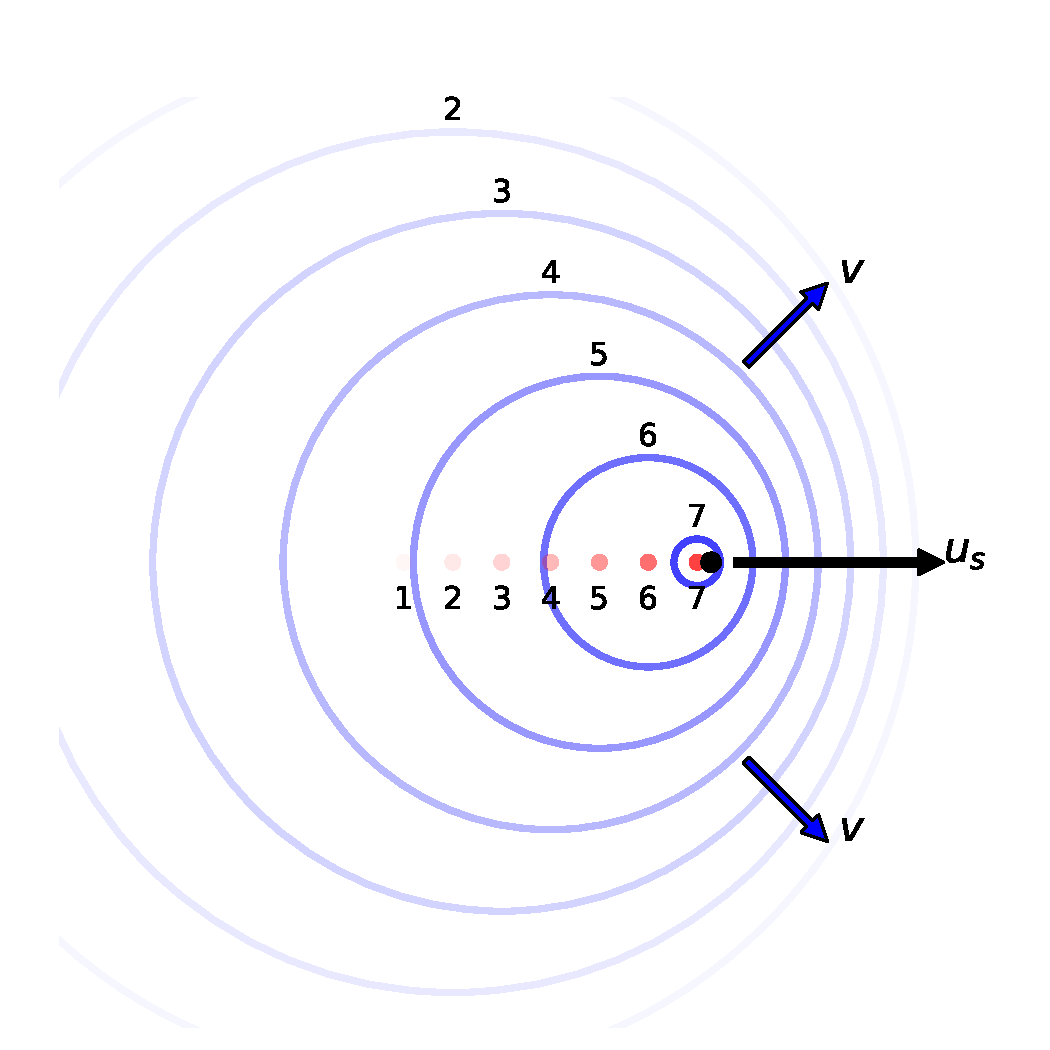
\includegraphics[width=0.7\linewidth]{visualisations/ch9-doppler2} 

}

\caption{We can look at this in more detail by showing where the dipper was for each of the spreading wavefronts. Here the dipper is moving forward at speed $u_r$, while the wavefronts spread out from their point of origin at speed $v$.}\label{fig:ch9-dopplerdipper2}
\end{figure}

This is a visual representation of a number of key statements:

\begin{itemize}
\tightlist
\item
  The speed of waves \(v\) in the medium is independent of the movement of the source;
\item
  The source produces waves at a frequency \(f_0\);
\item
  In a given time frame, \(\Delta t\), the source will emit \(N_s\) wavefronts, where:
  \begin{equation}
  N_s = f_0 \Delta t
  \end{equation}
\end{itemize}

From these statements, we can calculate the observed wavelength, \(\lambda^\prime\), by considering the relative distance travelled by the wave in a given timeframe and the number of waves produced by the source in that timeframe (Equation \eqref{eq:ch9-dopplereffect2}):

\begin{equation}
\lambda' = \frac{\textsf{relative distance}}{\textsf{no. of waves}} = \frac{(v\pm u_{s})\Delta t}{f_{0}\Delta t}
\label{eq:ch9-dopplereffect2}
\end{equation}

We can now consider two extremes; the observed wavelength in front of the source (to the right in the diagram), and the observed wavelength behind the source (to the left in the diagram):

\begin{equation}
\begin{array}{rcl}
\lambda^\prime_{\textsf{behind}} = \dfrac{v+u_{s}}{f_{0}} && \lambda^\prime_{\textsf{in front}} = \dfrac{v-u_{s}}{f_{0}}
\end{array}
\label{eq:ch9-dopplereffect3}
\end{equation}

We can now determine the frequency observed by using these expressions for the wavelength. Firstly, we determine the number of wavefronts passing the observer in the timeframe \(\Delta t\):

\begin{equation}
N_{\textsf{obs}} = \frac{v_{\textsf{obs}}\Delta t}{\lambda'}
\label{eq:ch9-dopplereffect4}
\end{equation}

\ldots where \(v_{\textsf{obs}}\) is the speed of the waves relative to the observer; i.e.~\(v_{\textsf{obs}} = v \pm u_{\textsf{obs}}\) ; where \(u_{\textsf{obs}}\) corresponds to the observer moving to the right in the diagram (as this reduces the relative velocity bewteen the observer and the wave). We can now rewrite the expression in Equation \eqref{eq:ch9-dopplereffect4} in terms of the phase velocity \(v\) and the relative speed of the observer, \(u_{\textsf{obs}}\):

\begin{equation}
N_{\textsf{obs}} = \frac{v \pm u_{\textsf{obs}}\Delta t}{\lambda'}
\label{eq:ch9-dopplereffect5}
\end{equation}

\ldots and finally we have the observed frequency \(f^\prime\) of a source in motion:

\begin{equation}
f^\prime = \frac{N_{\textsf{obs}}}{\Delta t} = \frac{v\pm u_{\textsf{obs}}}{\lambda'}
\label{eq:ch9-dopplereffect6}
\end{equation}

When we combine this with the equation for \(\lambda^\prime\), we obtain the general result (Equation @ref\{eq:ch9-dopplereffect7\})

\begin{equation}
f' = \left(\frac{v\pm u_{\textsf{obs}}}{v\pm u_{s}}\right)f_{0}\quad\textsf{or}\quad f' = \left(\frac{1\pm \frac{u_{\textsf{obs}}}{v}}{1\pm \frac{u_{s}}{v}}\right)f_{0}
\label{eq:ch9-dopplereffect7}
\end{equation}

It is important to pay attention to the signs when using the above equations; it can be easy to confuse the positive directions. The sign convention can help with this:

\begin{itemize}
\tightlist
\item
  The direction from the observer towards the source is positive
\end{itemize}

You can check your results using the principles:

\begin{itemize}
\tightlist
\item
  The observed frequency \(f'\) \textbf{increases} when the source and observer approach each other;
\item
  The observed frequency \(f'\) \textbf{decreases} when the source and observer move apart.
\end{itemize}

\hypertarget{sec:ch10-superposition}{%
\chapter{Superposition and Standing Waves}\label{sec:ch10-superposition}}

\emph{Textbook link: Tipler and Mosca, Section 15.1}

\hypertarget{sec:ch10-superposharmonic1}{%
\section{Superposition of harmonic waves}\label{sec:ch10-superposharmonic1}}

In Section \ref{sec:ch6-wavepulses} we showed that the wave equation (eq. \eqref{eq:ch6-waveequation1}) is satisfied by any function in the form \(y = f(x \pm vt)\). We can go further than this, and specify general expressions which can satisfy the wave equation.

Specifically, if we have two functions, \(y_1\) and \(y_2\) (Equation \eqref{eq:ch10-superposition1}), which satisfy the wave equation, then their sum (Equation \eqref{eq:ch10-superposition2}, including scaling constants \(C_1\) and \(C_2\)) must also satisfy the wave equation.

\begin{equation}
\begin{array}{rcl}
y_1 &=& A_1 \sin\left[k_1(x \pm vt)\right] \\
y_2 &=& A_2 \sin\left[k_2(x \pm vt)\right] \\
\end{array}
\label{eq:ch10-superposition1})
\end{equation}

\begin{equation}
y_3 = C_1 y_1 + C_2 y_2
\label{eq:ch10-superposition2}
\end{equation}

Using double angle formulae we can demonstrate that \(y_3\) can also be written in the form \(y = f(x \pm vt)\), thus satisfying the wave equation.\footnote{When including scaling factors, this can become less than trivial, but can still be done.} Therefore, the new wave \(y_3\) is a linear superposition of the original waves \(y_1\) and \(y_2\).

It is worth remembering that the wave equation was derived in the case of small amplitude disturbances; therefore if the vibration amplitudes become too large, the principle of superposition may fail. This can lead to some very interesting effects, including \textbf{non-linear optics}\footnote{Related to the non-linear response of the electromagnetic interactions with the medium, rather than light travelling in straight lines!}

\hypertarget{sec:ch10-identicalwaves1}{%
\section{Two waves with same amplitude and frequency}\label{sec:ch10-identicalwaves1}}

Let's now consider two waves with the same amplitude and frequency; but differing in phase (Equation \eqref{eq:ch10-superposition3}):

\begin{equation}
\begin{array}{rcl}
y_1 &=& y_0 \sin (kx - \omega t) \\
y_2 &=& y_0 \sin (kx - \omega t +\delta ) \\
\end{array}
\label{eq:ch10-superposition3}
\end{equation}

If the two waves are superimposed, for example if they are travelling through the same medium, the resultant wavefunction is just the sum of \(y_1\) and \(y_2\) (Equation \eqref{eq:ch10-superposition4}):

\begin{equation}
\begin{array}{rcl}
y &=& y_1 + y_2 \\
  &=& y_0 \sin (kx - \omega t) + y_0 \sin (kx - \omega t +\delta )
\end{array}
\label{eq:ch10-superposition4}
\end{equation}

In many situations it is mathematically simpler to use the complex exponential notation to treat waves and oscillations. However, in the case of a linear addition of two waves, it is simpler to just use trigonometric identities.

Here we will use the identity:

\begin{equation}
\sin\theta_{1}+\sin\theta_{2} = 2\sin\left(\frac{\theta_{1}+\theta_{2}}{2}\right)\cos\left(\frac{\theta_{1}-\theta_{2}}{2}\right)
\end{equation}

\ldots{} we obtain:

\begin{equation}
y = 2y_{0}\sin\left(kx-\omega t + \frac{\delta}{2}\right)\cos\left(\frac{-\delta}{2}\right)
\label{eq:ch10-superposition5}
\end{equation}

As an aside, we can do the same thing with complex notation; we can write our wave superposition as follows:

\begin{equation}
y = y_{1} + y_{2} =  y_{0}e^{i(kx - \omega t)} + y_{0}e^{i(kx - \omega t + \delta)}
\end{equation}

Remembering that we are interested in the `imaginary' component at the end since we started with \(y_1\) and \(y_2\) as sine waves, we can write this superposition as:

\begin{equation}
y = y_0 e^{i(kx-\omega t)}\left( 1 + \mathrm{e}^{\mathrm{i}\delta} \right)
\end{equation}

\begin{figure}

{\centering 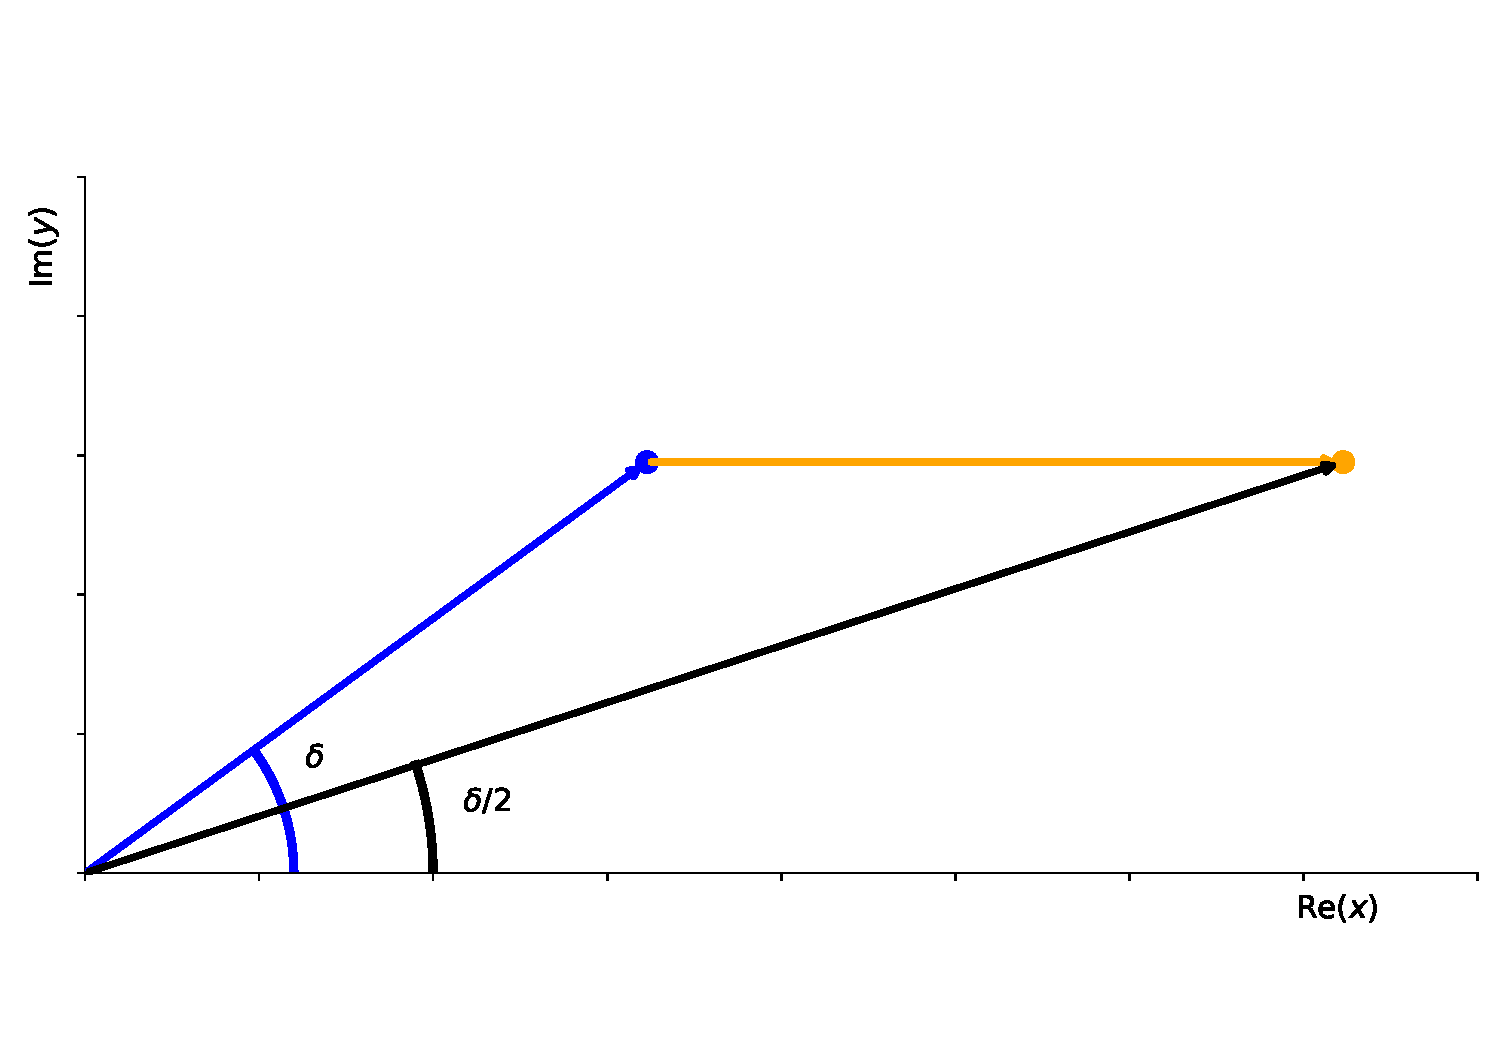
\includegraphics[width=0.7\linewidth]{visualisations/ch10-complexnumbers1} 

}

\caption{We can illustrate addition of complex numbers on an Argand diagram; here we show the sum $\left( 1 + \mathrm{e}^{\mathrm{i}\delta} \right)$; the result of this is the argument is halved from $\delta$ to $\frac{\delta}{2}$. }\label{fig:ch10-complexnumbers1}
\end{figure}

We can show using an Argand diagram (Figure \ref{fig:ch10-complexnumbers1}) that the term \((1 + \mathrm{e}^{\mathrm{i}\\delta})\) is equal to \(2\cos \left(\frac{\delta}{2}\right)e^{i\frac{\delta}{2}}\), and hence:

\begin{equation}
y = 2y_0 \cos(\delta/2) e^{i(kx-\omega t + \delta/2)}
\end{equation}

When we expand this expression using De Moivre's theorem, we obtain the same result as in Equation \eqref{eq:ch10-superposition5}:

\begin{equation}
y = \underbrace{2 y_0 \cos \left( \frac{\delta}{2} \right)}_{\textsf{New amplitude}} \underbrace{\sin \left( kx - \omega t + \frac{\delta}{2} \right)}_{\textsf{Travelling wave}}
\label{eq:ch10-superposition5b} 
\end{equation}

This tells us that the resulting wave has the same frequency as the component waves, but a different amplitude and phase. This new amplitude is given by the expression in Equation \eqref{eq:ch10-superposition5c}:

\begin{equation}
A_{\textsf{new}} = 2 y_0 \cos \left( \frac{\delta}{2} \right)
\label{eq:ch10-superposition5c} 
\end{equation}

There are three special cases to be aware of:

\begin{enumerate}
\def\labelenumi{\arabic{enumi}.}
\tightlist
\item
  If \(\delta = 0\), the waves are exactly in phase and the waves add together (constructive interference), with amplitude \(A = 2 y_0\);
\item
  If \(\delta = \pi\), the waves are exactly out of phase and the waves subtract (destructive interference), and the amplitude \(A = 0\);
\item
  If \(\delta = \frac{2\pi}{3}\), the resultant wave has exactly the same amplitude as the input waves.
\end{enumerate}

All three of these cases can be derived by substituting the relevant value of \(\delta\) into Equation \eqref{eq:ch10-superposition5c}.

\hypertarget{sec:ch10-standingwaves1}{%
\section{Standing waves}\label{sec:ch10-standingwaves1}}

A standing wave is a specific outcome which occurs when a wave is confined to space (for example on a piano string) and it reflects at the boundaries and travels back along its original path. This leads to waves travelling in both directions which combine by superposition. Only certain frequencies can exist in a standing wave, as the superposition leads to a stationary pattern called a \textbf{standing wave}.

\hypertarget{sec:ch10-standingwaves2}{%
\section{Wave function for a standing wave}\label{sec:ch10-standingwaves2}}

In order to fully consier a standing wave, we need to derive the form of its wavefunction. To do this, we consider two waves travelling in opposite directions along a string (Equation \eqref{eq:ch10-standingwaves1}). Because one is a reflection of the other (they each reflect from the boundaries), they will have the same frequency and phase.

\begin{equation}
\begin{array}{rcl}
y_1 &=& y_0 \sin (kx - \omega t) \\
y_2 &=& y_0 \sin (kx + \omega t) \\
\end{array}
\label{eq:ch10-standingwaves1}
\end{equation}

The resultant vertical displacement of the string is then the sum of these two waves (Equation \eqref{eq:ch10-standingwaves2}):

\begin{equation}
\begin{array}{rcl}
y &=& y_1 + y_2 \\
y &=& y_0 \sin (kx - \omega t) + y_0 \sin (kx + \omega t) \\
\end{array}
\label{eq:ch10-standingwaves2}
\end{equation}

We can add these directly using a trigonometric identify or we can work in the complex notation:

\begin{equation}
\begin{array}{rcl}
y &=& y_0 \sin (kx - \omega t) + y_0 \sin (kx + \omega t) \\
 &=& y_0 \mathrm{e}^{\mathrm{i}(kx - \omega t)} + y_0 \mathrm{e}^{\mathrm{i}(kx + \omega t)} \\
 &=& y_0 \mathrm{e}^{\mathrm{i}kx} \left( \mathrm{e}^{-\mathrm{i}\omega t} + \mathrm{e}^{\mathrm{i}\omega t} \right)
\end{array}
\label{eq:ch10-standingwaves3}
\end{equation}

We can use either an Argand diagram or De Moivre's theorem to show that the term \(\left( \mathrm{e}^{-\mathrm{i}\omega t}+ \mathrm{e}^{\mathrm{i}\omega t} \right) = 2 \cos \omega t\), and hence:

\begin{equation}
y = 2 y_0 \cos \omega t \mathrm{e}^{\mathrm{i}kx}
\end{equation}

We can now expand the complex exponent using De Moivre's theorem again and, remembering we are interested in the `imaginary' component (as this contains the desired sine function), and we obtain the result in Equation \eqref{eq:ch10-standingwaves4}:

\begin{equation}
y = \underbrace{2 y_0 \cos \omega t}_{\textsf{time-dependent amplitude}} \underbrace{\sin kx}_{\textsf{static wave}}
\label{eq:ch10-standingwaves4}
\end{equation}

This result describes a static wave, \(y = \sin kx\) whose amplitude varies in time as \(A = 2 y_0 \cos \omega t\). Note that it is possible to obtain this result via a trigonometric identity also.

\begin{figure}

{\centering 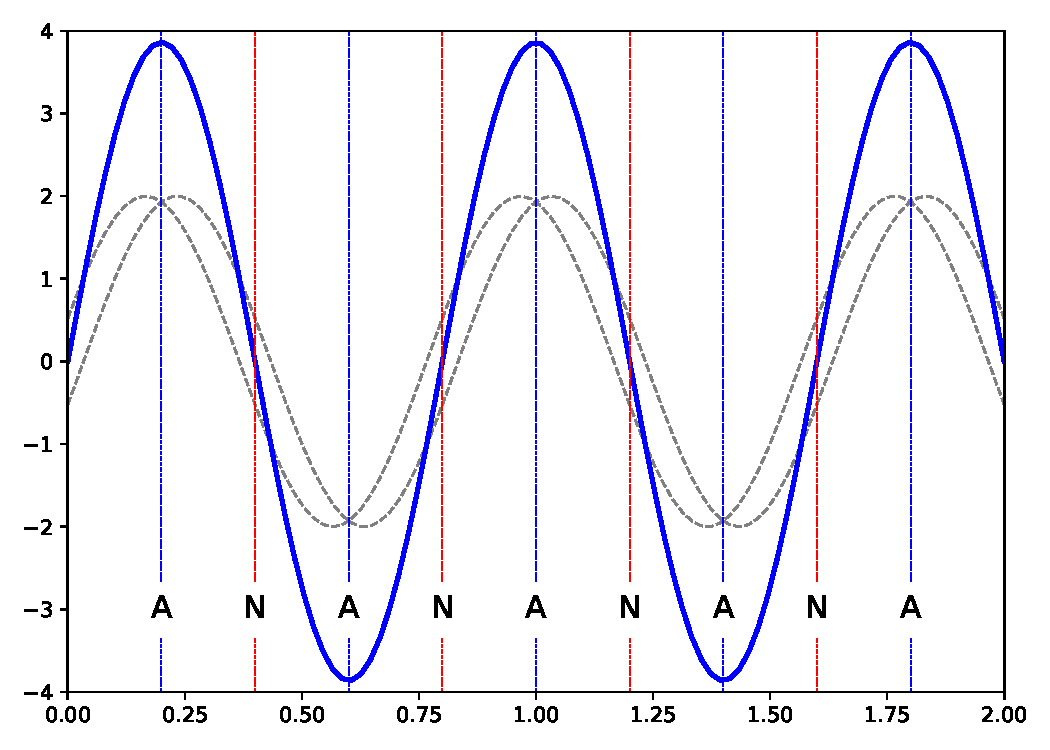
\includegraphics[width=0.7\linewidth]{visualisations/ch10-standingwave-n5} 

}

\caption{A standing wave is the result of two waves equal in frequency and amplitude moving past each other. This forms a static wave whose amplitude varies in time, and has nodes (N) and antinodes (A) present in the waveform. Here we show the fifth harmonic; 5 antinodes and a wavelength $\lambda = 2/5 = 0.8$.}\label{fig:ch10-standingwave1}
\end{figure}

This standing wave is illustrated in Figure \ref{fig:ch10-standingwave1}; but we notice that there are boundary conditions enforced; namely that the ends of the string are fixed at a constant, zero displacement; \emph{i.e.}:

\begin{itemize}
\tightlist
\item
  \(y = 0\) at \(x = 0\), and:
\item
  \(y = 0\) at \(x = L\) at all times \(t\)
\end{itemize}

\ldots where \(L\) is the length of the string. From this we deduce that \(\sin kL = 0\) and therefore there are a family of solutions for \(k\) and \(\lambda\), known as harmonics.

\begin{itemize}
\tightlist
\item
  If \(\sin kL = 0\), then \(kL = 0, \pi, 2\pi, \dots\), or \(k_n L = n\pi\)
\item
  Additionally, \(\lambda_n = \frac{2\pi}{k_n} = \frac{2L}{n}\) where \(n = 1, 2, 3, \dots\)
\end{itemize}

In other words, the vibrational modes are **quantised* due to the boundary conditions.

\hypertarget{sec:ch10-fixedstring1}{%
\section{Waves on strings fixed at both ends}\label{sec:ch10-fixedstring1}}

We have described the mathematics of standing waves; let's now apply this to a wave travelling on a string which is fixed at both ends. Figure \ref{fig:ch10-stringfundamental1} illustrates the fundamental wavelength of the string, which corresponds to twice the length of the string.

\begin{figure}

{\centering 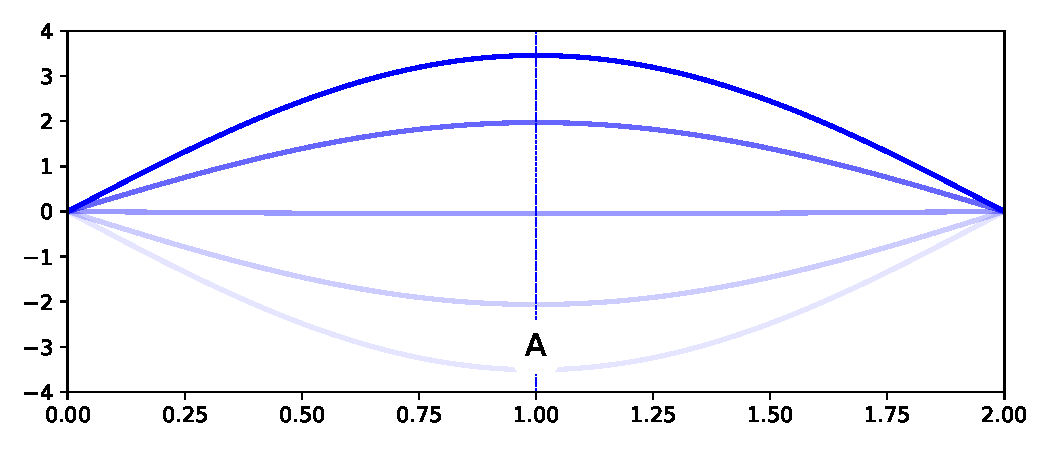
\includegraphics[width=0.7\linewidth]{visualisations/ch10-standingwave_stages-n1} 

}

\caption{The fundamental frequency, or first harmonic. This is one half-wavelength enclosed in the boundaries and has a single antinode.}\label{fig:ch10-stringfundamental1}
\end{figure}

We can then visualise the harmonics within the standing wave on this fixed string (Figure \ref{fig:ch10-stringharmonics1})

\begin{figure}

{\centering 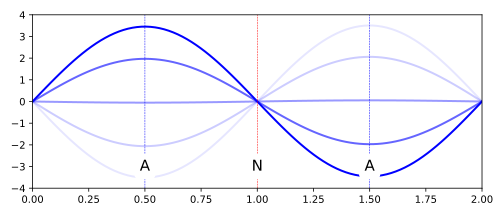
\includegraphics[width=0.7\linewidth]{visualisations/ch10-standingwave_stages-n2} 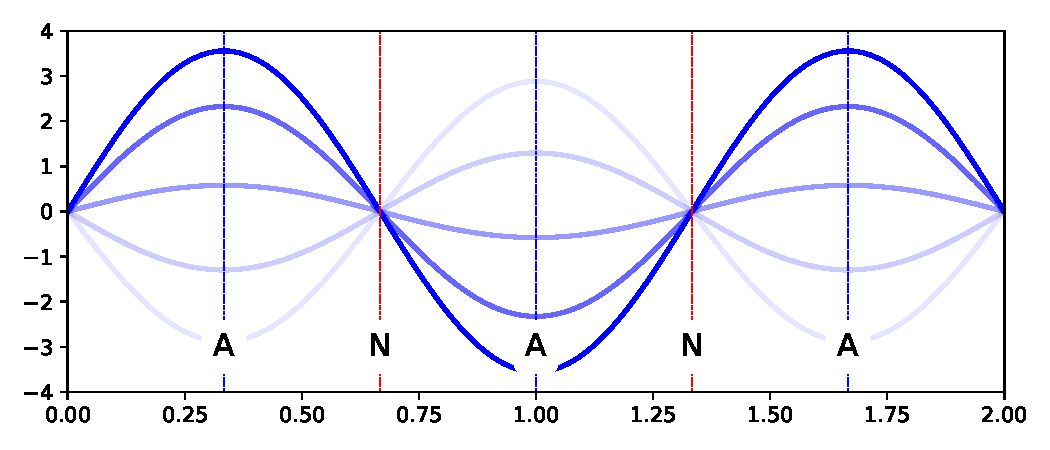
\includegraphics[width=0.7\linewidth]{visualisations/ch10-standingwave_stages-n3} 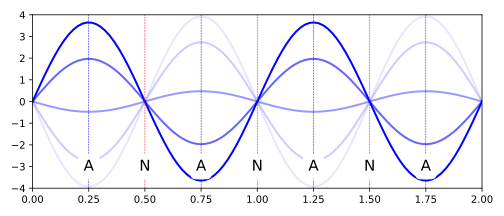
\includegraphics[width=0.7\linewidth]{visualisations/ch10-standingwave_stages-n4} 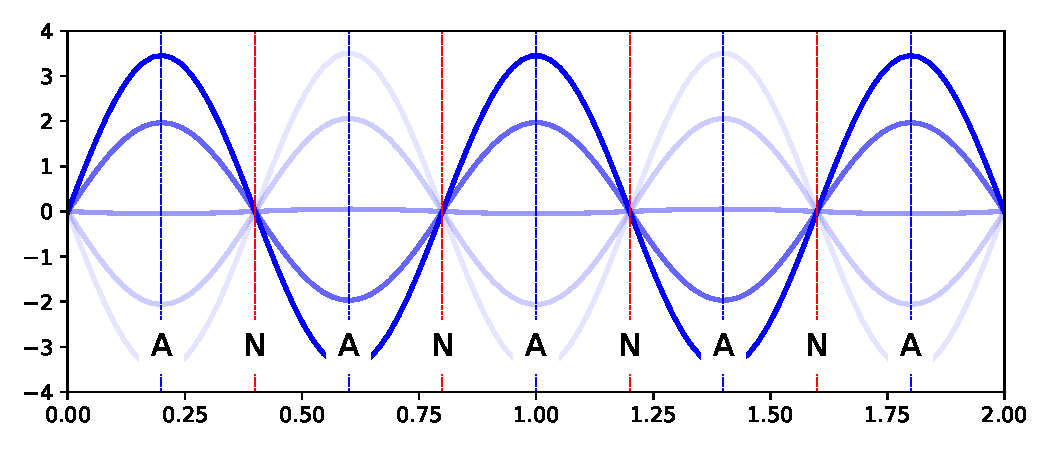
\includegraphics[width=0.7\linewidth]{visualisations/ch10-standingwave_stages-n5} 

}

\caption{The second, third, fourth and fifth harmonics of a standing wave on a string. Notice that the $n$th harmonic has $\frac{n}{2}$ wavelengths contained in the space.}\label{fig:ch10-stringharmonics1}
\end{figure}

The modes of vibration (resonances) shown in Figure \ref{fig:ch10-stringharmonics1} illustrate the occurence of \textbf{nodes} (points which do not move) and \textbf{antinodes} (points with the maximum vibration amplitudes). Note also that the end-points of the string must be nodes as well, as these points are fixed.

In general, the \(n\)th harmonic will have \(\frac{1}{n} \times\) wavelength and \(n \times\) the frequency of the fundamental vibration shown in Figure \ref{fig:ch10-stringfundamental1}.

\begin{longtable}[]{@{}lll@{}}
\caption{\label{tab:ch10-standingfrequencies} Showing the variation of wavelength and frequency of each harmonic with respect to the first (fundamental) wave.}\tabularnewline
\toprule
Harmonic & \(\lambda\) & \(f\)\tabularnewline
\midrule
\endfirsthead
\toprule
Harmonic & \(\lambda\) & \(f\)\tabularnewline
\midrule
\endhead
Fundamental, first & \(2L\) & \(f_1\)\tabularnewline
Second & \(L\) & \(2f_1\)\tabularnewline
Third & \(\frac{2L}{3}\) & \(3f_1\)\tabularnewline
Fourth & \(\frac{L}{2}\) & \(4f_1\)\tabularnewline
Fifth & \(\frac{2L}{5}\) & \(5f_1\)\tabularnewline
\(n\)th & \(\frac{2L}{n}\) & \(nf_1\)\tabularnewline
\bottomrule
\end{longtable}

In general, for the \(n\)th harmonic:

\begin{itemize}
\tightlist
\item
  Wavelength is given by \(\lambda_n = \frac{2L}{n}\)
\item
  Frequency is given by \(f = nf_1 = \frac{nv}{\lambda_1} = \frac{nv}{2L}\)
\end{itemize}

\ldots where \(v\) is the phase velocity (the speed of propagation of the wave along the string).

The resonant frequencies, or harmonics, of the string are known as its natural frequencies. Any string will resonate with maximum amplitude when excited with these frequencies, and this set of harmonics are known as a harmonic series. The actual harmonics heard when the string is excited will depend on the manner of its excitation; \emph{e.g.} a string plucied at its centre will \emph{only} display the odd harmonics; \emph{i.e.} those with an anti-node in the centre.

In stringed instruments (violin, piano, guitar etc.) the vibration of the string is amplified by a mechanical resonator; a soundboard in the case of the piano, or resonant cavities for a guitar or violin. These resonators must be carefully designed to resonate equally well over a wide range of frequencies.

\hypertarget{sec:ch10-pipesandwindinstruments}{%
\section{Organ pipes and other wind instruments}\label{sec:ch10-pipesandwindinstruments}}

In contrast to a vibrating string, wind instruments rely on a resonance within a column of air. We can model these pipes as a simple pipe, resonating at its natural frequencies when air is blown into (or across) an opening at one end. The resonant behaviour will differ depending on whether the other end of the pipe is open or closed. We will consider each of these cases in turn.

\hypertarget{pipes-open-at-both-ends}{%
\subsection{Pipes open at both ends}\label{pipes-open-at-both-ends}}

In this model, the column of air is able to vibrate at its ends, so we have a similar set of harmonics as for a string, but with displacement antinodes at its ends (the air can vibrate freely at the ends of the tube). There is a second set of nodes/antinodes corresponding to the pressure; these do not align with the displacement nodes/antinodes; rather a \textbf{pressure node} aligns with a \textbf{displacement antinode} and vice versa. (if an air molecule does not move, we have a displacement node, but it is continuously `squashed' from both sides by the oscillating air molecules, so experiences the biggest pressure change).

\begin{figure}

{\centering 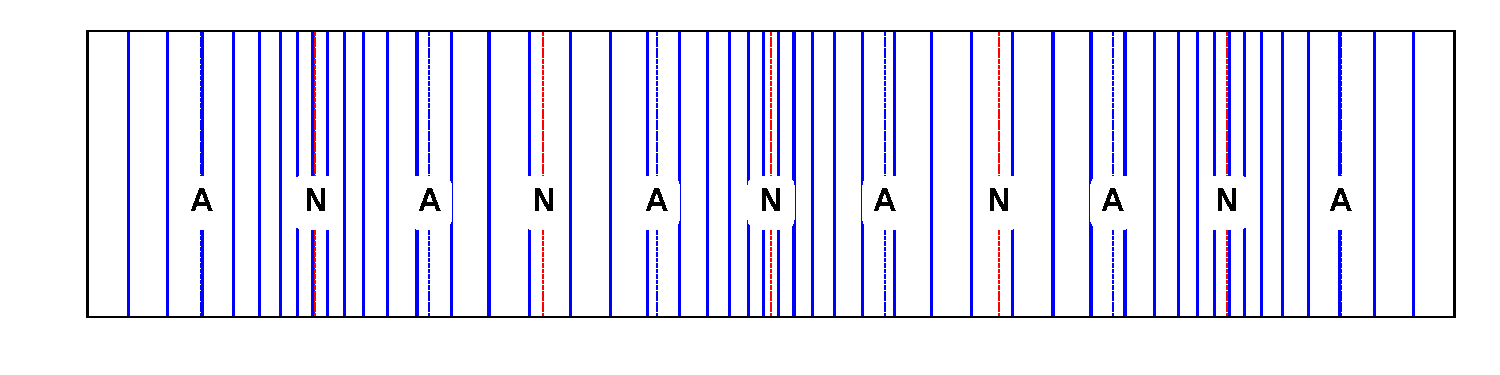
\includegraphics[width=0.7\linewidth]{visualisations/ch10-longitudinal-standingwave-n6closed} 

}

\caption{This image shows the node/antinode structure of a standing wave in a closed tube. Note the presence of a displacement node at either end where molecules are compressed against the end of the tube }\label{fig:ch10-waves-closedtube}
\end{figure}

We observe \textbf{all} harmonics in this system; there are no concerns about `position of plucking' that there is for the string. The displacement of the air molecules extends a little beyond the ends of the tube, so the effective length is given by \(L_\textsf{eff} = L + \Delta L\), where \(\Delta L\) is a small end correction. Therefore:

\begin{equation}
\lambda_n = \frac{2L_\textsf{eff}}{n} \quad \textsf{and} \quad f_n = \frac{nv}{2L_\textsf{eff}}
\end{equation}

\hypertarget{pipe-closed-at-one-end}{%
\section{Pipe closed at one end}\label{pipe-closed-at-one-end}}

We now have a different situation with different boundary conditions:

\begin{itemize}
\tightlist
\item
  There must be a displacement node at the closed end
\item
  There must be a displacement antinode at the open end
\end{itemize}

This now gives us a fundamental wavelength four times longer than the effective length of the tube (the shortest node-antinode separation is a quarter wavelength).

This means that we only observe the \textbf{odd} harmonics (the even harmonics would not allow the boundary conditions for this tube).

\begin{figure}

{\centering 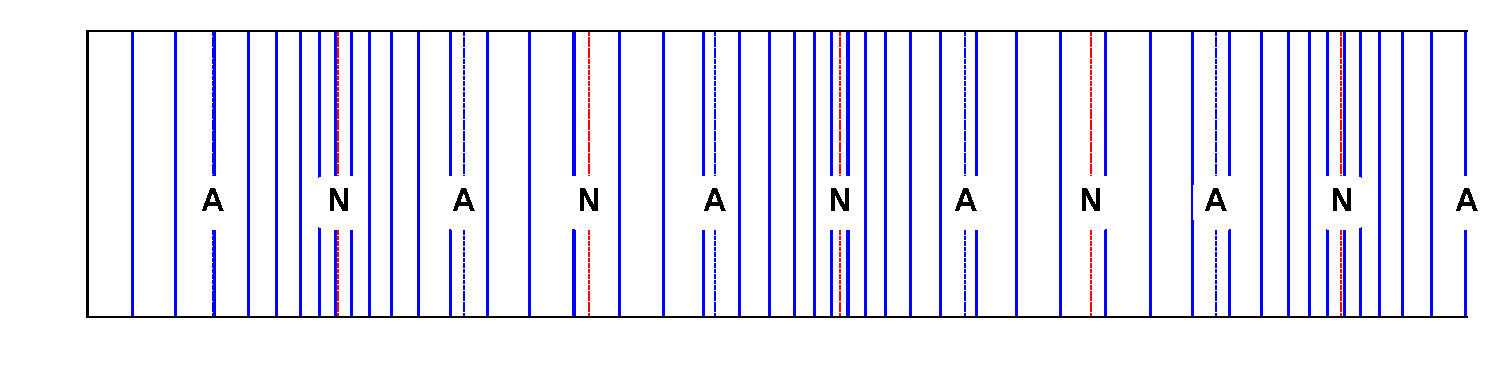
\includegraphics[width=0.7\linewidth]{visualisations/ch10-longitudinal-standingwave-n6open} 

}

\caption{For a tube open at one end, the standing waves now have a node at the closed end, and an antinode at the open end. This changes the available harmonics within the tube.}\label{fig:ch10-waves-opentube}
\end{figure}

\begin{equation}
\lambda_n = \frac{4 L_\textsf{eff}}{n} \quad n = 1,3,5,\dots
\end{equation}

\begin{equation}
f_n = \frac{nv}{4 L_\textsf{eff}} \quad n = 1,3,5,\dots
\end{equation}

\hypertarget{sec:ch11-fourieranalysis}{%
\chapter{Fourier analysis}\label{sec:ch11-fourieranalysis}}

Any vibrating string such as those in stringed musical instruments contain a range of different harmonics all drawn from the harmonic series. The exact combination of harmonics will vary depending on the way the string is set in motion; \emph{e.g.} a violin string is bowed, while a piano string is struck. The resulting sound wave will be a complicated periodic function, and not obviously a sine wave. The fundamental theorem of Fourier analysis is that \textbf{any} periodic function can be constructed by a linear superposition of sine and cosine waves. A corollary to this is that any periodic waveform can therefore be \emph{constructed} using a linear superposition of sine and cosine waves. The set of sines and cosines used to represent a function in Fourier analysis is referred to as a \emph{Fourier series}, and the set of constants in the series are known as \emph{Fourier coefficients}.

The standard form for a Fourier series representation of a function \(P(t)\) with period \(T\) is:

\begin{equation}
\begin{array}{rclcl}
P(t) = \dfrac{1}{2}a_0 & +& a_1 \cos \omega t &+& b_1 \sin \omega t \\
                      & + &a_2 \cos 2\omega t &+& b_2 \sin 2\omega t \\
                      & +& a_3 \cos 3\omega t &+& b_3 \sin 3\omega t \\
\end{array}
\end{equation}

\ldots or, to express as a summation:

\begin{equation}
P(t) = \frac{1}{2}a_{0} + \sum_{n=1}^{\infty}\left(a_{n}\cos n\omega t + b_{n}\sin n\omega t\right)
\end{equation}

\ldots where \(\omega = \frac{2\pi}{T}\)

The presence of both sine and cosine terms allows the relative phase of each component to be controlled:

\begin{itemize}
\tightlist
\item
  If \(P(t)\) is an \textbf{even function}, only \textbf{cosine} terms are required;
\item
  Similarly, only \textbf{sine} terms are required if the function is \textbf{odd}
\end{itemize}

The Fourier coefficients \(a_0\), \(a_1\), \(a_2\) etc. are given by:

\begin{equation}
a_n = \frac{2}{T} \int_{-\frac{T}{2}}^{\frac{T}{2}} P(t) \cos n \omega t ~\mathrm{d}t \quad n = 0,1,2,3 \dots
\end{equation}

\begin{equation}
b_n = \frac{2}{T} \int_{-\frac{T}{2}}^{\frac{T}{2}} P(t) \sin n \omega t ~\mathrm{d}t \quad n = 1,2,3 \dots
\end{equation}

It can be seen that \(\frac{a_0}{2}\) is equal to the averave value of \(P(t)\) over one cycle.

\hypertarget{sec:ch11-squarewave}{%
\section{Example: the square wave}\label{sec:ch11-squarewave}}

Consider a square wave defined on the interval \(\left[-1,1 \right]\) by:

\begin{equation}
P(t) = \left\{ \begin{array}{rl} 1 & -\frac{1}{2} \leq t \leq \frac{1}{2} \\ 0 & \textsf{elsewhere} \end{array} \right.
\end{equation}

\begin{figure}

{\centering 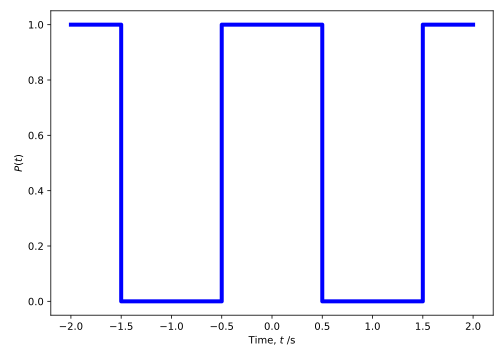
\includegraphics[width=0.7\linewidth]{visualisations/ch11-squarewave1} 

}

\caption{The form of a square wave; often termed a 'top hat' function. This is interpreted in electronics as a digital signal which is either on or off.}\label{fig:ch11-squarewave1}
\end{figure}

The period of this function is 2 s, so that \(\omega = \pi\).

Since \(P(t)\) is an even function (\emph{i.e.} it has symmetry about the \(y\) axis), it follows from symmetry that \(b_1 = b_2 = b_3 = \dots = 0\). On the other hand, the cosine coefficients are given by:

\begin{equation}
\begin{array}{rcl}
a_0 &=& \displaystyle{\int_{-1}^{1}} P(t) \cos 0 \mathrm{d}t = \displaystyle{\int_{-\frac{1}{2}}^{\frac{1}{2}}} \mathrm{d}t = 1 \\
a_n &=& \displaystyle{\int_{-1}^{1}} P(t) \cos n \pi t \mathrm{d}t \\
    &=& \displaystyle{\int_{-\frac{1}{2}}^{\frac{1}{2}}} P(t) \cos n \pi t \mathrm{d}t \\
    &=& \dfrac{2}{n\pi} \sin \left( \frac{n\pi}{2} \right) \quad n = 1, 2, 3, \dots
\end{array}
\end{equation}

Thus, we find the following:

\begin{itemize}
\tightlist
\item
  \(a_0 = 1\)
\item
  \(a_1 = \frac{2}{\pi}\)
\item
  \(a_2 = 0\)
\item
  \(a_3 = -\frac{2}{3\pi}\)
\item
  \(a_4 = 0\)
\item
  \(a_5 = \frac{2}{5\pi}\)
\item
  \(a_6 = 0\)
\item
  \(\dots\)
\end{itemize}

\ldots and the Fourier series is given by:

\begin{equation}
P(t) = \frac{1}{2} + \frac{2}{\pi}\left(\cos\pi t - \frac{\cos3\pi t}{3} + \frac{\cos5\pi t}{5} -\ldots\right)
\end{equation}

As we increase the number of terms in the series, we see out wave comes closer and closer to the square wave we sketched earlier.

\begin{figure}

{\centering 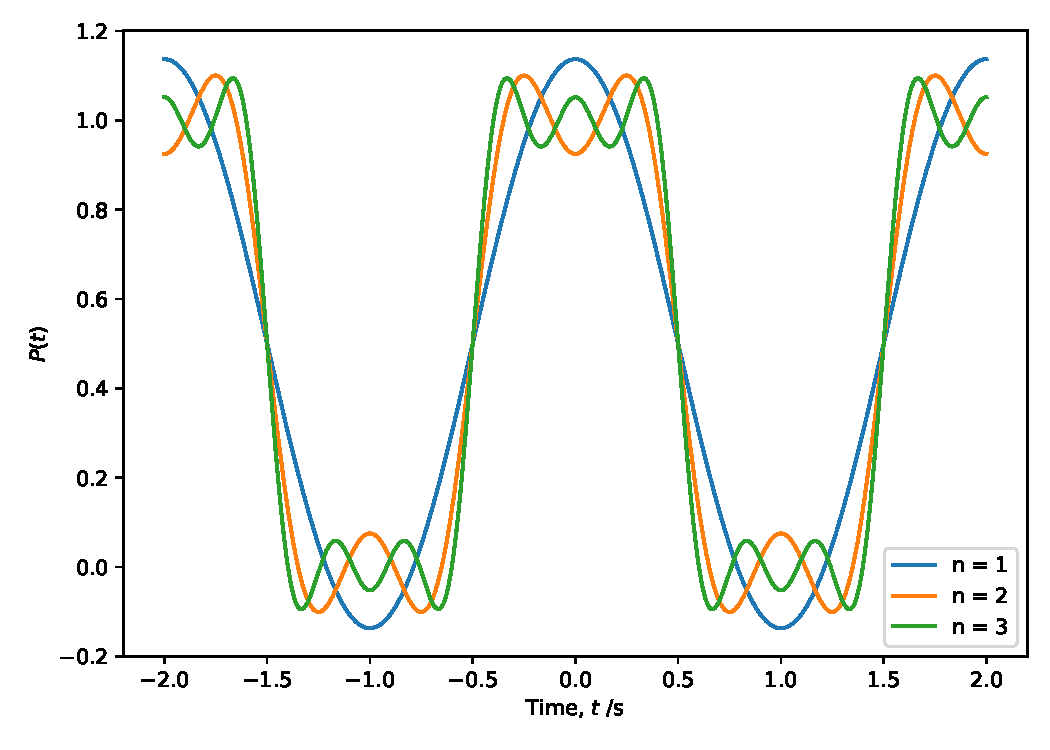
\includegraphics[width=0.7\linewidth]{visualisations/ch11-fouriersum5} 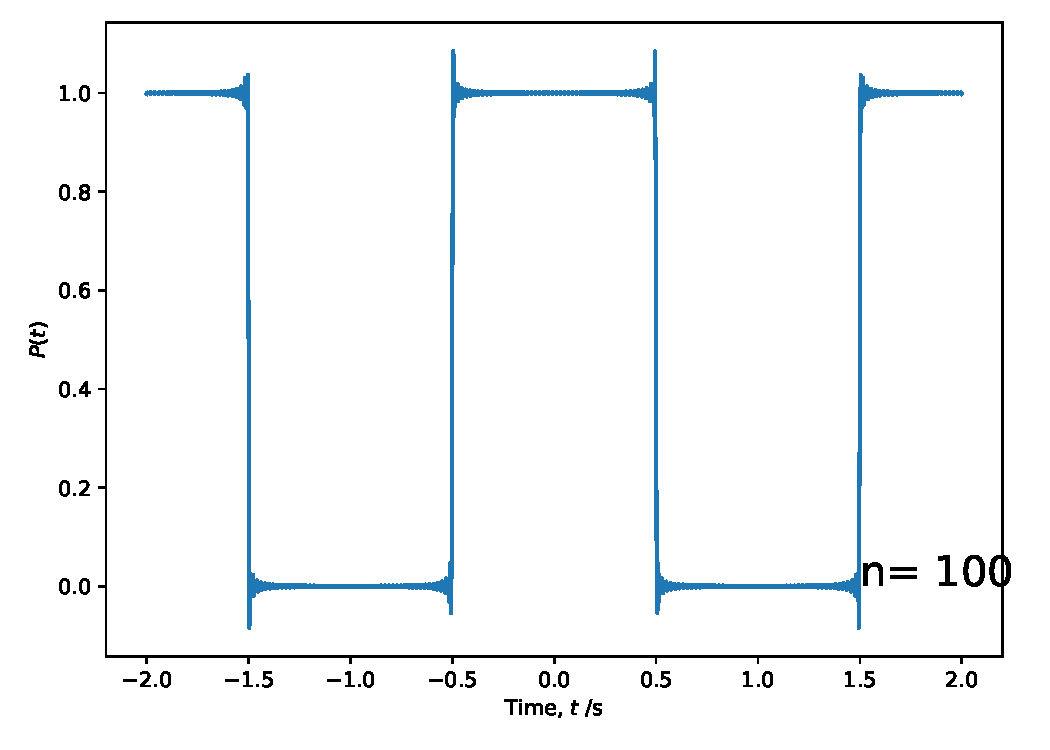
\includegraphics[width=0.7\linewidth]{visualisations/ch11-fouriersum100} 

}

\caption{As we add increasing numbers of terms to the Fourier summation, our collection of sinusoidal waves converges on the form of the 'top hat' function.}\label{fig:ch11-fouriersum5}
\end{figure}

A square wave can be thought of as the most extreme deviation from a sinusoidal function; yet we have demonstrated that we can reconstruct a square wave from a linear superposition of sinusoidal wave forms. Using these principles, we can build any waveform from a linear superposition of sinusoidal waves.

\hypertarget{sec:ch11-harmonicwavemakeup1}{%
\section{The harmonic makeup of any wave}\label{sec:ch11-harmonicwavemakeup1}}

We have shown using the example of the square wave that any wave can be made of the sum of harmonic sinusoidal components, each with a characteristic amplitude. Once again, let's consider the example of musical instruments. When two different wind instruments play the same note, (concert A, 440 Hz), they naturally sound different; the oboe sounds distinctly different to a clarinet, however they are, ostensibly, playing a note with the same frequency. The reason they sound different is because the wave which comes out of each has a fundamentally differnet form; the \textbf{tone quality}.

The wave-forms for the oboe and clarinet are shown in Figure \ref{fig:ch11-oboeclarinetwaveform1}, where, despite having the same fundamental frequency, the waveform is considerably more complex than that of a tuning fork (a `nearly pure' wave form with no additional harmonics).

\begin{figure}

{\centering 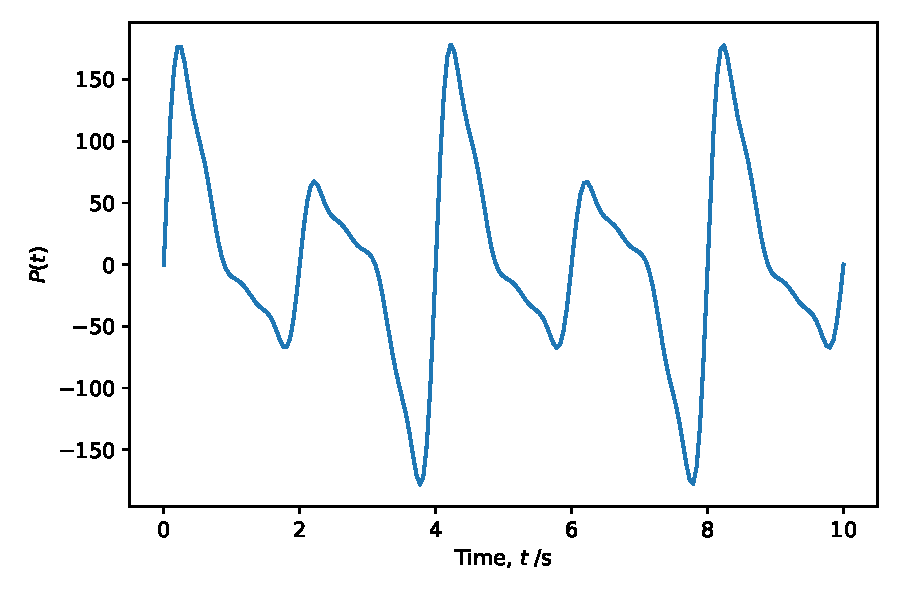
\includegraphics[width=0.7\linewidth]{visualisations/slides-harmonicsum_oboe} 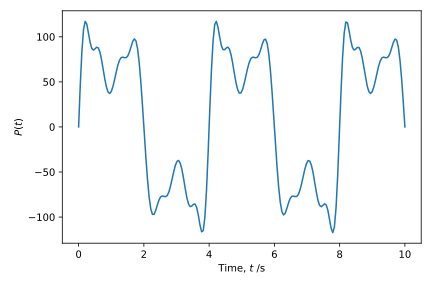
\includegraphics[width=0.7\linewidth]{visualisations/slides-harmonicsum_clar} 

}

\caption{We have an illusration of the waveforms for an oboe (top) and clarinet(bottom); these are both playing the same frequency, but we see a very different harmonic makeup.}\label{fig:ch11-oboeclarinetwaveform1}
\end{figure}

These waveforms can be analysed in terms of the relative contributions from each of the harmonics in the harmonic series, and we can see in Figure \ref{fig:ch11-oboeclarinetharmonics} that the contributions from each of the harmonics in the harmonic series is quite different between the two. The shapes of the tubes for each of the instruments leads to different contributions from the harmonics in each instrument, and this shapes the distinctive sound we hear. The real trick of course is identifying what this harmonic makeup is from the presented waveform. This is the essence of Fourier analysis; identifying the harmonic makeup of a given waveform, and has applications way beyond musical instruments!

\hypertarget{sec:ch11-fouriertransforms}{%
\section{Fourier Transforms}\label{sec:ch11-fouriertransforms}}

A Fourier transform is a mathematical tool which allows for the identification of the component frequencies and corresponding amplitude of a given waveform. It is a tool which is used in almost area of instrumental analysis, and its importance cannot be understated. The principles of the Fourier transform are as follows:

\begin{itemize}
\tightlist
\item
  If a period of oscillation is allowed to become infinite (\emph{i.e.} the wave becomes non-periodic), we can calculate the spectral density (the amplitude of each contributing harmonic wave) of any non-periodic function \emph{e.g.} a wave pulse.
\item
  In this limit the Fourier coefficients become continuous functions \emph{i.e.} all frequencies are allowed;
\item
  The (infinite) array of Fourier coefficients is referred to as the \textbf{Fourier Transform} of the function
\item
  Thus, we can show that \textbf{any} arbitrary wave pulse can be produced from a superposition of harmonic waves, which is why we attach such importance to understanding their behaviour.
\end{itemize}

\hypertarget{sec:ch11-importantfouriertransforms}{%
\section{Some important Fourier transforms}\label{sec:ch11-importantfouriertransforms}}

\hypertarget{sec:ch11-ftcosine}{%
\subsection{A cosine wave}\label{sec:ch11-ftcosine}}

\begin{figure}

{\centering 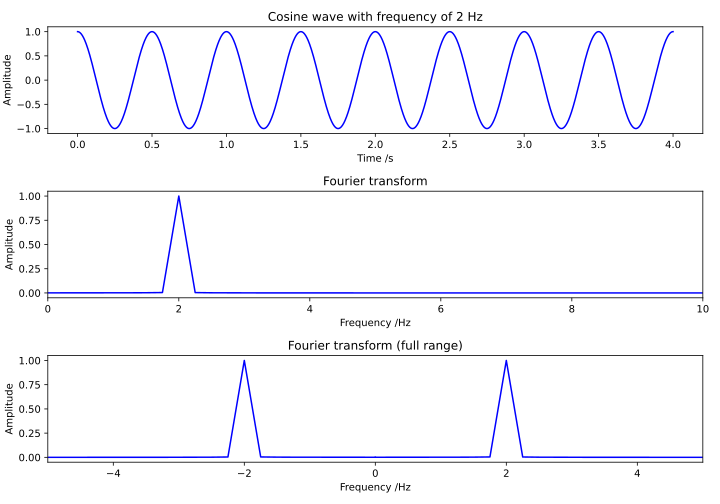
\includegraphics[width=0.7\linewidth]{visualisations/ch11-ftcosinefunction1} 

}

\caption{A periodic cosine function (top) made up of a single frequency gives a single 'spike' in the Fourier transform (bottom) at the appropriate frequency. Note that this Fourier transform has finite width because it is a genuine 'fast Fourier transform' performed in Python using data from a cosine plot; so is not the idealised 'infinitesimally narrow delta function' which it would otherwise be.}\label{fig:ch11-ftcosinefunction1}
\end{figure}

A pure cosine wave has a single frequency; the Fourier transform yields a single spike (a single Fourier coefficient) at this frequency. Strictly, there is also a spike at \(-\omega_0\) because the transform is symmetric.

\hypertarget{sec:ch11-fttophat}{%
\subsection{The `top hat' function}\label{sec:ch11-fttophat}}

\begin{figure}

{\centering \includegraphics[width=0.7\linewidth]{visualisations/ch11-fttophat1} 

}

\caption{A non-periodic 'top hat' function is made up of an infinite Fourier series, involving all frequencies. We see this reflected in the Fourier transform (bottom) where the tranform function extends to infinity.}\label{fig:ch11-fttophat1}
\end{figure}

A top-hat function is a wavepulse for a square wave, defined as a pulse width of \(\tau\). The Fourier transform yields a continuous series of Fourier coefficients, with defined positions along the frequency axis.

\hypertarget{sec:ch11-ftgaussian}{%
\subsection{A Gaussian function}\label{sec:ch11-ftgaussian}}

\begin{figure}

{\centering \includegraphics[width=0.7\linewidth]{visualisations/ch11-ftgaussian1} 

}

\caption{The Fourier tranform of a finite Gaussian function is another Gaussian function, but the width is a reciprical of the original function.}\label{fig:ch11-ftgaussian1}
\end{figure}

For a Gaussian function with full-width at half-maximum (FWHM) \(\tau\), its Fourier transform yields another Gaussian function, with FWHM = \(\frac{2\pi}{\tau}\). A Gaussian function is a good approximation to a laser pulse; the shorter the laser pulse, the more frequencies are required to generate it. This has ramifications on the colour of the pulse! (this is a subject for another course!)

\hypertarget{sec:ch11-bandwidththeorem}{%
\section{The Bandwidth Theorem}\label{sec:ch11-bandwidththeorem}}

\emph{Tipler and Mosca, 16.3}

The relationship between the widths of the two Gaussian functions shown in Section \ref{sec:ch11-ftgaussian} is important and has far-reaching consequences. If the Gaussian function represents a wave pulse with width (in time) \(\Delta t\), the Fourier transform tells us it contains a spread of frequencies, \(\Delta \omega\). However, the product \(\Delta t \Delta \omega\) is a constant:

\begin{equation}
\Delta t \Delta \omega = 2\pi
\end{equation}

This is known as the ``Bandwidth theorem'' and, if we examine the spatial width of the pulse (\(\Delta x\) rather than \(\Delta t\)) we see a similar relationship:

\begin{equation}
\Delta x \Delta k = 2\pi
\end{equation}

For a more general pulse shape, the determination of the width of the pulse becomes more arbitrary, and so the bandwidth theorem becomes:

\begin{equation}
\Delta t \Delta \omega \approx 2\pi \quad \textsf{and} \quad \Delta x \Delta k \approx 2\pi
\end{equation}

There are a number of implications of the bandwidth theorem:

\begin{itemize}
\tightlist
\item
  A \textbf{narrow} wave pulse will contain a \textbf{wide} range of frequencies;
\item
  A \textbf{broad} wave pulse will contain a \textbf{narrow} range of frequencies'
\item
  \(\Delta \omega = 0\) implies that \(\Delta t = \infty\); \emph{i.e.} an infinite sine wave with a single frequency - a perfect wave;
\item
  Similarly, \(\Delta k = 0\) implies \(\Delta x = \infty\).
\end{itemize}

\hypertarget{sec:ch12-wavepackets}{%
\chapter{Wave packets and Dispersion}\label{sec:ch12-wavepackets}}

\emph{Textbook link: Tipler and Mosca, Section 16.3}

A \textbf{wave packet} is exactly what it sounds like; a ``parcel'' containing a group of waves all of different frequencies. How these wave packets travel will vary depending on the properties of the medium through which they travel. If all the frequency components of the wave packet (or wave pulse) travel with the same phase velocity, \(v_p\), the resulting disturbance propagates without changing shape and the medium is known as a \textbf{non-dispersive medium}. If, however, frequency components travel at different speeds through the medium, we have a \textbf{dispersive} medium. You will have likely observed the effects of a dispersive medium; if you have ever stood at a quiet railway platform (usually underground), you can hear the tell-tale sound of an approaching train from the ``pinging'' sound in the rails long before you hear the actual vehicle itself as the high-frequencies travel faster through the rail than the lower frequencies.

The velocity of propagation of the packet is known as the \textbf{group velocity} \(v_g\), the velocity at which energy is carried through the medium. In a non-dispersive medium, this is equal to the phase velocity \(v_p\). If the medium is \textbf{dispersive} however, different frequencies travel with different values of \(v_p\), and the wavepacket spreads as it travels; this is the origin of the `pinging' sound we hear in railway tracks.

\begin{figure}

{\centering \includegraphics[width=0.7\linewidth]{visualisations/ch12-wavepacketdispersion1} 

}

\caption{As a wave packet travels through a dispersive medium in which higher frequencies travel faster than lower frequencies, the wave packet 'spreads out' in space.}\label{fig:ch12-dispersionillustration1}
\end{figure}

\hypertarget{sec:ch12-twowavesbeats1}{%
\section{Two waves, same amplitude, different frequency (Beats)}\label{sec:ch12-twowavesbeats1}}

Let's consider two waves with the same amplitude but differing in frequency (\emph{i.e.} amplitude \(y_0\) is common to both, each has independent frequency \(\omega_1\) and \(\omega 2\)). For convenience we will assume that the phase difference between the two is zero at time \(t=0\), and we will then consider their displacements at an arbitrary \(x\) coordinate (\emph{e.g.} \(x=0\)).

Firstly, let's lay out the mathematical description of each wave:

\begin{equation}
y_{1} = y_{0} \sin \omega_{1} t \quad \textsf{and} \quad y_{2} = y_{0} \sin \omega_{2} t
\label{eq:ch12-addtwowavebeats1}
\end{equation}

We can now obtain an expression for the overall observed amplitude, \(y = y_1 + y_2\), and use the standard trigonometric identities\footnote{Here we use the sum-to-product identity \(\sin A + \sin B = 2\cos \left(\frac{A-B}{2}\right) \sin\left(\frac{A+B}{2}\right)\)} to combine the two equations:

\begin{equation}
\begin{array}{rcl}
y &=& y_1 + y_2 \\
 &=& y_{0} \sin \omega_{1} t +  y_{0} \sin \omega_{2} t \\
 &=& 2y_{0}\cos\left(\dfrac{\omega_{1}-\omega_{2}}{2}t\right)\sin\left(\dfrac{\omega_{1}+\omega_{2}}{2}t\right)
\end{array}
\label{eq:ch12-addtwowavebeats2}
\end{equation}

As an aside, we can achieve the same result by using complex exponentials where the sum of the two waves is given in Equation \eqref{eq:ch12-addtwowavebeats1}, where we are interested in the imaginary component since we started with sine waves:

\begin{equation}
y = y_0 \mathrm{e}^{\mathrm{i}\omega_1 t} + y_0\mathrm{e}^{\mathrm{i}\omega_2 t}
\label{eq:ch12-addtwowavebeats3}
\end{equation}

These can be added on an Argand diagram to show the result in Equation \eqref{eq:ch12-addtwowavebeats4}

\begin{equation}
y = y_0 r\mathrm{e}^{\mathrm{i}\theta}
\label{eq:ch12-addtwowavebeats4}
\end{equation}

\ldots where:

\begin{equation}
r = 2 \cos\left(\frac{\omega_1t - \omega_2t}{2}\right) \quad \textsf{and} \quad \theta = \frac{\omega_1 t + \omega_2 t}{2}
\end{equation}

Our end result if we expand this complex representation is:

\begin{equation}
y = 2 y_0 \cos \left( \frac{\omega_1t - \omega_2t}{2} \right) \mathrm{e}^{\mathrm{i}\left(\frac{\omega_1 t + \omega_2t}{2} \right)}
\end{equation}

As we said above, we are interested in the `imaginary' (sine) component, and we end up with the same result as shown in Equation \eqref{eq:ch12-addtwowavebeats2}. We can simplify the expression as in Equation \eqref{eq:ch12-addtwowavebeats5}.

\begin{equation}
y = \underbrace{ 2y_{0} \cos \left( \frac{\Delta \omega}{2}t \right)}_{\textsf{slowly varying amplitude}} \underbrace{ \sin \omega_{av}t}_{\textsf{wave with average frequency}}
\end{equation}

\ldots where \(\Delta \omega = \omega_1 - \omega_2\).

The frequency fo the resulting wave is the average of the two input waves, while the amplitude oscillates with frequency \(\frac{\Delta \omega}{2}\). This is known as \textbf{beating}. The actual frequency of the beats themselves is twice this, as shown in Figure \ref{fig:ch12-oscillationbeats1}.

\begin{figure}

{\centering \includegraphics[width=0.7\linewidth]{visualisations/ch12-beats1} 

}

\caption{As two waves interfere with each other ($f_1 = 3.0$ Hz; $f_2 = 3.2$ Hz), we see the interference structure as a waveform of frequency 3.1 Hz with a slowly varying amplitude at frequency 0.1 Hz (the 'envelope'). This visualises the 'beats' in the interference structure.}\label{fig:ch12-oscillationbeats1}
\end{figure}

Therefore, if the frequency of the slowly varying amplitude is \(\frac{\Delta \omega}{2}\), the observed frequency of the `beats' will be twice this; \emph{i.e.} the difference in frequency between the two sources.

Repeating the analysis above but with the full expressions for the two sine waves (\emph{i.e.} \(y_n = y_0 \sin(kx - \omega t)\)), we obtain the expession in Equation \eqref{eq:ch12-addtwowavessine1}

\begin{equation}
y= 2 y_{0} \cos \left (\frac{\Delta kx - \Delta\omega t}{2}\right) \cdot \sin(k_\textsf{av}x - \omega_\textsf{av}t )
\label{eq:ch12-addtwowavessine1}
\end{equation}

From Equation \eqref{eq:ch12-addtwowavessine1} we find there are two velocities to consider; the phase velocity of the ``average'' wave, and the phase velocity of the ``envelope'' (the waveform which describes the amplitude; see Figure \ref{fig:ch12-oscillationbeats1}). These are laid out below:

The phase velocity of the ``average'' wave:

\begin{equation}
v_{av} = \frac{\omega_{av}}{k_{av}}
\end{equation}

The phase velocity of the envelope:

\begin{equation}
v_{env} = \frac{\Delta\omega}{\Delta k}
\end{equation}

In a \emph{non-dispersive} medium (\emph{i.e.} all frequencies travel with the same phase velocity), it can be shown that \(v_{\textsf{av}} = v_{\textsf{env}} = \frac{\omega_1}{k_1} = \frac{\omega_2}{k_2} =\) the phase velocity of the medium.

However, in a dispersive medium, the velocities are not equal, \emph{i.e.} \(v_av \neq v_env\), and the ``envelope'' propagates at a different speed to the individual components. We associate \(v_env\) with the group velocity \(v_g\) and in this case would be represented as:

\begin{equation}
v_{g} = \frac{\Delta\omega}{\Delta k}
\end{equation}

\hypertarget{sec:ch12-dispersion}{%
\section{Dispersion}\label{sec:ch12-dispersion}}

As has already been mentioned, in a \textbf{dispersive} medium, \(v_p\) is different for every frequency component, and the group velocity is not equal to the initial phase velocity \(v_p\); \emph{i.e.} \(v_g \neq v_p\). For any dispersive medium, we can write a relationship between \(\omega\) and \(k\) so that \(\omega\) varies as a function of \(k\); \emph{i.e.} \(\omega = \omega(k)\). This is called the \textbf{dispersion relation} and depends on the physics of the particular wave phenomena being observed.

In the general case, the group velocity is given by the derivative of the dispersion relation (Equation \eqref{eq:ch12-dispersion1}). The proof of this relation is available in some advanced textbooks, but it is not necessary for this course.

\begin{equation}
v_g \equiv \frac{\partial w(k)}{\partial k}
\label{eq:ch12-dispersion1}
\end{equation}

For a non-dispersive medium, \(\omega\) is directly proportional to \(k\) (Equation \eqref{eq:ch12-dispersion2})

\begin{equation}
w(k) = v_p k \quad \textsf{with} \quad v_p = \textsf{constant}
\label{eq:ch12-dispersion2}
\end{equation}

The consequence of this is that, when the function is differentiated according to the principle in Equation \eqref{eq:ch12-dispersion1}, we find that \(v_g = v_p\) (Equation \eqref{eq:ch12-dispersion2b}) as has been mentioned previously.

\begin{equation}
v_g \equiv \frac{\partial w(k)}{\partial k} = \frac{\mathrm{d} (v_p k)}{\mathrm{d}k} = v_p
\label{eq:ch12-dispersion2b}
\end{equation}

For a dispersive medium however, \(v_p\) becomes a function of \(k\). If we consider a simple case where \(\omega\) has a linear dependence on k (Equation \eqref{eq:ch12-dispersion3}) with constant terms \(a\) and \(b\):

\begin{equation}
\omega = ak + b
\label{eq:ch12-dispersion3}
\end{equation}

As before, the phase velocity is still defined as \(v_p = \frac{\omega}{k} = a + \frac{b}{k}\), while the group velocity is found by differentiation (Equation \eqref{eq:ch12-dispersion4}):

\begin{equation}
v_g = \frac{\partial w(k)}{\partial k} = a
\label{eq:ch12-dispersion4}
\end{equation}

We wee that these expressions for the phase velocity \(v_p = a + \frac{b}{k}\) and the group velocity \(v_g = a\) are different; therefore the envelope of the wave packet will move at a different speed from the phase velocity of the wave. However, the group velocity is still the same for all wavenumbers \(k\).

When \(\omega\) is a more general function of \(k\), the group and phase velocities will each depend differently on \(k\). The dependence of the group velocity on \(k\) means that envelope doesn't move at a single velocity and its components of different wavenumber (or wavelength) have different velocities, distorting the envelope.

So-called \emph{normal dispersion} occurs when the group velocity is lower than the phase velocity (\(v_g < v_p\)); this is the most common situation, however it is possible to have \emph{anomalous dispersion} in which the group velocity, and hence the energy, travels faster than the individual waves.

Examples of dispersion include:

\begin{itemize}
\tightlist
\item
  Splitting of light by prism
\item
  Formation of a rainbow
\item
  Phonons propagating through a crystalline solid
\item
  Spreading of light pulses in fibre-optic cables. The dispersion limits the maximum length of cable before signal reconditioning is needed.
\end{itemize}

\hypertarget{sec:ch12-waterwaves}{%
\section{Water waves}\label{sec:ch12-waterwaves}}

The dispersion relation for water is given in Equation \eqref{eq:ch12-waterdispersion1}, which includes the acceleration due to gravity (\(g\)) and the depth of the water (\(h\)):

\begin{equation}
\omega^2 = gk\tanh(kh)
\label{eq:ch12-waterdispersion1}
\end{equation}

For shallow water and/or long wavelengths, \(kh \ll 1\) and \(tanh(kh) \simeq kh\). This allows Equation \eqref{eq:ch12-waterdispersion1} to be simpified to:

\begin{equation}
\omega^2 \simeq gk \cdot kh \quad \textsf{and} \quad \omega \simeq k \sqrt{gh}
\end{equation}

We can then detemrine the phase velocity \(\v_p\) in this situation as:

\begin{equation}
v_p = \frac{\omega}{k} = \sqrt{gh}
\end{equation}

\ldots and there is \textbf{no dispersion} (the phase velocity has no variable dependences). This applies in the case of the tsunami, where the water depth is small compared to the wavelength, even when crossing oceans. This means that these waves are able to propagate over global distances without significantly changing shape.

For intermiediate depths, we might use the expansion of \(\tanh(x)\) to write this term as:

\begin{equation}
\tanh(kh) = kh - \frac{(kh)^3}{3} + \cdots
\end{equation}

\ldots from which we obtain:

\begin{equation}
\omega^2 \simeq gk \cdot \left(kh - \frac{(kh)^3}{3} \right)
\end{equation}

We can now use this to determine the phase velocity of the wavepacket in water (Equation \eqref{eq:ch12-waterdispersion2}):

\begin{equation}
v_p = \frac{\omega}{k} = \frac{\sqrt{gh}}{\sqrt{1+\frac{(kh)^2}{3}}}
\label{eq:ch12-waterdispersion2}
\end{equation}

Equation \eqref{eq:ch12-waterdispersion2}) tells us that the dispersion of the wave increases with increasing water depth relative to the wavelength.

\hypertarget{sec:ch12-phonondispersion}{%
\section{Sound waves in a crystal (phonons)}\label{sec:ch12-phonondispersion}}

When we consider sound-waves in a crystal, we can consider both longitudinal sound waves as well as transverse sound waves (as we are not in a fluid, a transverse wave is now possible due to the intermolecular forces within the crystal).

We will first consider the one-dimensional case, as the three dimensional case can be derived from the principles laid out here. Firstly, let's consider what a wave might look like when propagating along a one-dimensional crystal. We imagine our one-dimensional lattice to be a line of molecules, all connected by a ``spring'' (to model the molecular bond). In this model, we can either have a longitudinal wave, where the springs are stretched and compressed as the molecules oscillate in the direction of the crystal axis, or we can have a transverse wave, in which the 1-D line of molecules behaves as a string. These are illustrated in Figure \ref{fig:ch12-phononvibration1}.

\begin{figure}

{\centering \includegraphics[width=0.7\linewidth]{visualisations/ch12-phonons1} 

}

\caption{A 1 dimensional lattice can carry sound waves (phonons, also known as lattice vibrations) via both transverse and longitudinal vibrational modes. }\label{fig:ch12-phononvibration1}
\end{figure}

From this model, it can be shown that the phase velocity can be given by the relationship shown in Equation \eqref{eq:ch12-phononvibration1}, relating the tension in the 1-D lattice (\(F\)), the linear density of the 1-D lattice (\(\mu\)) and the periodicity of the lattice, \(a\).

\begin{equation}
v_{p} = \frac{\omega}{k} = \frac{F}{\mu}\frac{\sin \left(\frac{ka}{2}\right)}{\frac{ka}{2}}
\label{eq:ch12-phononvibration1}
\end{equation}

In the long-wavelength limit, \(k \rightarrow 0\) and \(v_p \rightarrow \frac{F}{\mu}\).

Additionally, we can rewrite Equation \eqref{eq:ch12-phononvibration1} to gain an expression for \(\omega\):

\begin{equation}
\omega = \frac{kF}{\mu}\frac{\sin \left(\frac{ka}{2}\right)}{\frac{ka}{2}} = \frac{2F}{a\mu}\sin \left(\frac{ka}{2}\right)
\label{eq:ch12-phononvibration2}
\end{equation}

If we plot the angular frequency \(\omega\) against the wavenumber \(k\), we obtain the \textbf{dispersion curve}, shown in Figure \ref{fig:ch12-dispersioncurve1}.

\begin{figure}

{\centering \includegraphics[width=0.7\linewidth]{visualisations/ch12-dispersioncurve1} 

}

\caption{The variation in angular frequency $\omega$ with wavenumber $k$ in a dispersive medium. There is an upper limit to the wavenumber which the medium can sustain, namely $\pi / a$}\label{fig:ch12-dispersioncurve1}
\end{figure}

From Equation \eqref{eq:ch12-phononvibration2}, we can find the group velocity \(v_g\) by differentiation:

\begin{equation}
v_g = \frac{\mathrm{d}\omega}{\mathrm{d}k} = \frac{F}{\mu} \cos \left(\frac{ka}{2}\right)
\label{eq:ch12-phononvibration3}
\end{equation}

Once again, examination of Equation \eqref{eq:ch12-phononvibration3} shows:

\begin{itemize}
\tightlist
\item
  The group velocity, \(v_g\) tends to \(\frac{F}{\mu}\) as \(k \rightarrow 0\); and:
\item
  The group velocity also drops to zero when \(k = \frac{\pi}{a}\)
\end{itemize}

At the point when \(k = \frac{\pi}{a}\), alternate atoms move in exact anti-phase, and we have the appearance of a standing wave (Figure \ref{fig:ch12-dispersionlattice1}). Therefore there is an effective cut-off at \(k = \frac{\\pi}{a}\); waves with a greater wave number than this (shorter wavelength, higher frequency) cannot be supported by the lattice.\footnote{This is a similar effect to the aliasing obserfved in sample signals in Experiment S}

\begin{figure}

{\centering \includegraphics[width=0.7\linewidth]{visualisations/ch12-phonons2} 

}

\caption{When the wavenumber $k = \pi / a$, the atoms move in perfect anti-phase and the movement appears as a standing wave. The lattice can no longer support a higher wavenumber than this.}\label{fig:ch12-dispersionlattice1}
\end{figure}

Note that the periodicity of the lattice, \(a\) (also known as the molecular spacing) is typically around \(10^{-9} - 10^{-10}\) m, so this effect will only be observed for \textbf{very} high frequencies.

\hypertarget{sec:ch13-interference}{%
\chapter{Interference and Diffraction}\label{sec:ch13-interference}}

\hypertarget{sec:ch13-conditionsinterference}{%
\section{Conditions for interference}\label{sec:ch13-conditionsinterference}}

In Section \ref{sec:ch10-identicalwaves1}, we discussed the principle of superposition of two waves with the same frequency and wavelength in the context of forming a standing wave. Specifically, we found that the resultant wave has an amplitude which depends on the phase difference.

Mathematically, for two waves described by \(y_1\) and \(y_2\), we obtain the result shown below (from Equation \eqref{eq:ch10-superposition5b}):

\begin{equation}
y_1 = A_0 \sin(k r - \omega t) \quad \textsf{and} \quad y_2 = A_0 \sin(k r - \omega t + \delta)
\end{equation}

\begin{equation}
y = \underbrace{2 A_0 \cos \left( \frac{\delta}{2} \right)}_{\textsf{New amplitude}} \underbrace{\sin \left( kr - \omega t + \frac{\delta}{2} \right)}_{\textsf{Travelling wave}}
\end{equation}

Therefore the amplitude \(A\) of the resultant wave may be described by:

\begin{equation}
A = 2 A_0 \cos \left( \frac{\delta}{2} \right)
\label{eq:ch13-amplitudeinterfere1}
\end{equation}

This amplitude \(A\) is a maximum when the waves are \emph{in phase} (\(\delta = 2m\pi\)), and at a minimum when the waves are \emph{out of phase} (\(\delta = (2m+1)\pi\)).

Typically, a phase difference between identical waves results from a path difference; for example two light waves travelling by different routes. For such a path difference, \(\Delta r\), the phase difference is given by \(\delta = \frac{2 \pi \Delta r}{\lambda}\). In the case of \textbf{constructive} interference, \(\delta = 2m\pi\) and \(\Delta r = m\lambda\), while for \textbf{destructive} interference \(\delta = (2m+1)\pi\) and \(\Delta r = \left(m+\frac{1}{2}\right)\lambda\).

For any two waves to interfere, they must be \textbf{coherent}; \emph{i.e.} there must be a fixed phase relationship between the two sources. This is usually achieved by splitting a single light source. Light sources such as tungsten filament bulbs are \textbf{not} coherent; the emission results from thermal excitation and the different componetns of the bulb radiate independently of one another. A LASER on the other hand \textbf{is coherent}; the beam is produced by stimulated emission, a process which only occurs if all photons are in phase.

\hypertarget{sec:ch13-lightpropagation}{%
\section{Propagation of Light - Huygens's Principle}\label{sec:ch13-lightpropagation}}

Huygens' Principle is summarised as follows:

\begin{quote}
Each point on a primary wavefront serves as a source of spherical secondary wavelets, which advance with a speed and frequency equal to those of the primary wave. The primary wavefront at some later time is the envelope of these wavelets.
\end{quote}

While the propagation of light is in fact goverened by Maxwell's equations, Huygens' construction provides an extremely valuable way of analysing diffraction problems. An illustration of Huygens' principle is shown in Figure \ref{fig:ch13-huygenswavelets1}; we only consider the \emph{forward moving} portion of the wavelet, not the whole spherical wavelet.

\begin{figure}

{\centering \includegraphics[width=0.7\linewidth]{visualisations/ch13-huygenswavelets1} 

}

\caption{The Huygens' wavelet construction. A wavefront is considered to be a source of secondary wavelets; each subsequent wavefront is the envelope of the forward moving component of the wavelets.}\label{fig:ch13-huygenswavelets1}
\end{figure}

\hypertarget{sec:ch13-twoslitinterference}{%
\section{The two-slit interference pattern}\label{sec:ch13-twoslitinterference}}

\emph{Tipler and Mosca, 33.3}

Consider a double slit experiment, where uniform coherent waves approach a pair of slits in a barrier (Figure \ref{fig:ch13-doubleslit1}). According to Huygens' Principle, each slit then becomes a source of wavelets, which then radiate outwards from this point and, since the wavelets from each source are coheret, they then interfere.

\begin{figure}

{\centering \includegraphics[width=0.7\linewidth]{visualisations/LaTeX/ch13-doubleslits} 

}

\caption{The configuration of the double slit experiment. Two narrow slits are separated at distance $d$, each of which becomes a source of secondary wavelets which can then create the interference pattern.}\label{fig:ch13-doubleslit1}
\end{figure}

If we examine the path of waves travelling in an arbitrary direction from each slit which converge on the observation screen (Figure \#ref(fig:ch13-doubleslit2)), we can start to consider the behaviour of our wavelets.

\begin{figure}

{\centering \includegraphics[width=0.7\linewidth]{visualisations/LaTeX/ch13-doubleslits2} 

}

\caption{Looking at the whole double slit experiment, we can determine the angles within the experiment and define the observation position $X$ on the screen as a function of these angles. Under the Fraunhofer condition (long field interference), the rays can be considered parallel, allowing the path difference and hence phase offset to be determined.}\label{fig:ch13-doubleslit2}
\end{figure}

If we assume that the distance to the screen \(L\) is considerably larger than the distance between the slits \(d\) then, since \(L \gg d\), then we can say that the angles \(\theta_1\), \(\theta_2\) and \(\theta\) are approxiamtely equal (\emph{i.e.} \(\theta_1 \approx \theta_2 \approx \theta\)); the Fraunhofer diffraction condition.

Note that when \(L \simeq d\), this approximation no longer applies and the diffraction becomes very complex, and is termed \textbf{Fresnel conditions}. For the purposes of this discussion we will only consider the Fraunhofer case (\emph{i.e.} \(L \gg d\)).

We can obtain an expression for the path difference between the waves; if we are assuming that the distance to the screen is so large the rays may be considered parallel, then the path difference may be determined from Figure \ref{fig:ch13-doubleslit2}:

\begin{equation}
\begin{array}{rclrcll}
d\sin\theta &=& m\lambda \quad; & m &=& 0,1,2, \dots &\textsf{for maxima} \\
d\sin\theta &=& \left(m + \frac{1}{2}\right) \lambda \quad; & m &=& 0,1,2, \dots &\textsf{for minima}
\end{array}
\end{equation}

At point \(P\) on the observation screen we can then determine the phase difference, \(\delta\):

\begin{equation}
\delta = \frac{2\pi}{\lambda}d\sin\theta
\end{equation}

However, remember that, as \(L \gg d\), then \(\sin \theta \approx \tan \theta = \frac{X}{L}\) for small \(\theta\). Therefore, at points where interference maxima are observed (\emph{i.e.} \(d\sin\theta = m\lambda\)):

\begin{equation}
d\sin\theta = \frac{d X_m}{L}= m\lambda \quad \textsf{and} \quad X_m = \frac{m\lambda L}{d}
\label{eq:ch13-fraunhoferderiv1}
\end{equation}

Equation \eqref{eq:ch13-fraunhoferderiv1} tells us that the distance of the ``\(m\)''th maximum from the midpoint of the diffraction pattern scales only with the value of \(m\); all other values being constant for the particular experimental setup; \emph{i.e.} the maxima will be \textbf{equally spaced}.

We can also consider the intensity of the fringes; from our work in Section \ref{sec:ch7-transportenergypower}, the intensity (the transmitted power) is proportional to the square of the amplitude. Using the result shown in Equation \eqref{eq:ch13-amplitudeinterfere1}, we can derive the expression in Equation \eqref{eq:ch13-amplitudeinterfere2}:

\begin{equation}
I = A^2 = 4 A_0^2 \cos^2 \left(\frac{\delta}{2}\right)
\label{eq:ch13-amplitudeinterfere2}
\end{equation}

However, since we have the expression \(\delta = \frac{2\pi d}{\lambda}\sin\theta \approx \frac{2\pi d X}{\lambda L}\) the phase difference \(\delta\) is proportional to the distance of the fringe from the midpoint of the interference pattern, \(X\). Therefore, since \(\delta \propto X\), we expect to see fringes following the intensity of a \(\cos^2\) function (Figure \ref{fig:ch13-cos2fringes}).

\begin{figure}

{\centering \includegraphics[width=0.7\linewidth]{visualisations/LaTeX/ch13-cos2-interference} 

}

\caption{The interference pattern from two narrow slits gives an intensity pattern proportional to a $\cos^2$ function.}\label{fig:ch13-cos2fringes}
\end{figure}

\hypertarget{sec:ch13-singlewideslit}{%
\section{Diffraction from a single wide slit}\label{sec:ch13-singlewideslit}}

Let's now turn to the effect of coherent plane wavefronts incident on a single wide slit (Figure \ref{fig:ch13-singlewideslit1}).

\begin{figure}

{\centering \includegraphics[width=0.7\linewidth]{visualisations/LaTeX/ch13-singlewideslit1} 

}

\caption{A single wide slit of width $d$ can be thought of as a source of many different wavelets; here we have shown three rays to give an indication of the complexity of the interference pattern.}\label{fig:ch13-singlewideslit1}
\end{figure}

In this situation, we imagine dividing the aperture into a set of secondary sources and use the Huygens' construction to consider secondary wavelets. These `diffracted waves' will appear to spread. To find the diffracted intensity in a particualr direction, we add to gether the secondary waves travelling in that direction, taking into account the path (and hence phase) differences.

We will conduct our analysis in two stages:

\begin{enumerate}
\def\labelenumi{\arabic{enumi}.}
\tightlist
\item
  We consider the superposition of waves from two secondary sources, symmetrically disposed about the centre of the slit, similar to the ``two narrow slit'' example above;
\item
  We then add together the contributions from all pairs of sources across the wide slit.
\end{enumerate}

The workthrough for this example is slightly involved, so is shown elsewhere, however we show the elements of the solution here and, as for the two narrow slits example above, use it to determine the amplitude of the superposition as a function of \(X\), the distance on screen.

\begin{figure}

{\centering \includegraphics[width=0.7\linewidth]{visualisations/LaTeX/ch13-singlewideslit2b} 

}

\caption{Construction of the diffraction pattern from a single wide slit involves looking at pairs of wavelets $\Delta x$; through quantifying the phase difference between these two wavelets and summing over the slit we can reconstruct the diffraction pattern.}\label{fig:ch13-singlewideslit2}
\end{figure}

The result of the derivation is that the superposition observed as a function of \(X\) is a travelling wave with amplitude as:

\begin{equation}
A \propto \mathrm{sinc}\left(\frac{\pi a X}{\lambda L}\right)
\end{equation}

\ldots where \(\mathrm{sinc}(x) = \frac{\sin (x)}{x}\).\footnote{The ``sinc'' function is used often in signal processing, and its name comes from its name the `sine cardinal' function, and is widely used in Fourier transforms.} Therefore the intensity (\(\propto A^2\)) observed on the screen is given by:

\begin{equation}
I \propto A^2 \propto \mathrm{sinc}^2 \left(\frac{\pi a X}{\lambda L}\right)
\label{eq:ch13-singlewideslit1}
\end{equation}

The positions of the dark fringes can then be determined by setting this equal to zero:

\begin{equation}
\begin{array}{rrcl}
&\mathrm{sinc}^2 \left(\frac{\pi a X}{\lambda L}\right) &=& 0 \\
\equiv & \dfrac{\sin^2 \left(\frac{\pi a X}{\lambda L}\right)}{x^2 }&=& 0 \\
& \sin^2 \left(\frac{\pi a X}{\lambda L}\right) &=& 0 \\
& \frac{\pi a X}{\lambda L} &=& \pi, 2\pi, 3\pi, \dots \equiv m \pi \\
& \frac{ a X}{\lambda L} &=& m , \textsf{where } m \neq 0
\end{array}
\label{eq:ch13-singlewideslit2}
\end{equation}

From Equation \eqref{eq:ch13-singlewideslit2}, we can determine that our dark fringes occur when the output of the sinc function in Equation \eqref{eq:ch13-singlewideslit1} is equal to zero; \emph{i.e.} dark fringes occur at \(X_m = \frac{m\lambda L}{a}\) where \(m = 1, 2, 3, \dots\), but \(m \neq 0\). Therefore the separation of the dark fringes, \(X_m\) is inversely proportional to the slit width \(a\), \emph{i.e} \(X_m \propto \frac{1}{a}\).

\hypertarget{sec:ch13-difftwowideslits}{%
\section{Diffraction from two wide slits}\label{sec:ch13-difftwowideslits}}

Once again, we have a series of coherent planar wavefronts approaching the barrier, this time with two wide slits present (Figure \ref{fig:ch13-twowideslits1}).

\begin{figure}

{\centering \includegraphics[width=0.7\linewidth]{visualisations/LaTeX/ch13-doubleslitswide1} 

}

\caption{The configuration for two wide slits of width $a$ at separation $b$ appears similar to the construction for narrow slits, except now each slit is a source of a number of wavelets, rather than a single wavelet. This has profound implications on the diffraction pattern observed.}\label{fig:ch13-twowideslits1}
\end{figure}

We can use the same method as was used previously, but with different limits of integration, and we obtain a travelling wave with amplitude as given in Equation \eqref{eq:ch13-twowideslits1}:

\begin{equation}
A = a A_0 \cos \left( \frac{\pi b X}{\lambda L} \right) \mathrm{sinc}\left( \frac{\pi a X}{\lambda L} \right)
\label{eq:ch13-twowideslits1}
\end{equation}

The corresponding intensity observed of the fringes observed on the screen is then as shown in Equation \eqref{eq:ch13-twowideslits2}:

\begin{equation}
I \propto A^2 = a^2 A_0^2 \cos^2 \left( \frac{\pi b X}{\lambda L} \right) \mathrm{sinc}^2 \left( \frac{\pi a X}{\lambda L}\right)
\label{eq:ch13-twowideslits2}
\end{equation}

In other words, the intensity is the product of the diffraction pattern from the two ``narrow'' slits with that from the single wide slit:

\begin{equation}
I \propto A^2 = \underbrace{a^2 A_0^2}_{\textsf{Constant scaling factors}} 
\underbrace{\cos^2 \left( \frac{\pi b X}{\lambda L} \right)}_{\textsf{Double slit intensity}} \underbrace{\mathrm{sinc}^2 \left( \frac{\pi a X}{\lambda L}\right)}_{\textsf{Wide slit intensity}}
\label{eq:ch13-twowideslits3}
\end{equation}

WHen we have two functions combined in this manner, we say that one is the `envelope' of the other - it effectively ``contains'' and controls the intensity of the other. In general, the lower frequency function is the `envelope', so here the \(\mathrm{sinc}^2\) function is the envelope of the \(\cos^2\) function. The intensities of this combined function are shown in Figure \ref{fig:ch13-twowideslits2}

\begin{figure}

{\centering \includegraphics[width=0.7\linewidth]{visualisations/ch13-doublewideslit1} 

}

\caption{The diffraction pattern from two wide slits is a combination of the result of a single wide slit and that of two narrow slits. The sinc$^{2}$ function becomes the envelope shaping the intensities of the peaks from the narrow slit solution.}\label{fig:ch13-twowideslits2}
\end{figure}

\hypertarget{sec:ch13-diffmultipleslits}{%
\section{Multiple slits with equal spacing}\label{sec:ch13-diffmultipleslits}}

Over the past few sections we have laid out the principles of diffraction and interference of light from a pair of narrow slits, a single wide slit, and a pair of wide slits. We have shown how the relative intensity functions are combined and how this gives us our intensity patterns for the combination of the two more simple examples. We can apply these principles to determine the expected interference patterns we would observe for multiple slit systems.

\hypertarget{sec:ch13-ftindiffraction}{%
\section{Fourier transforms in diffraction}\label{sec:ch13-ftindiffraction}}

The method we have used to determine the intensities of fringes in diffraction/interference patterns may be generalised for any aperture by introducing a general aperture function \(f(x)\) which describes the shape of the apterture (\emph{e.g.} if we have two narrow slits, we use two delta functions to describe them). We can then sum the phase components from all elements \(\Delta x\) across this aperture. The amplitude of the constant wave is then given by Equation \eqref{eq:ch13-ftindiffraction1}

\begin{equation}
A = \sum_{\textsf{aperture}} f(x) \mathrm{e}^{\mathrm{i}\delta(x)} \Delta x
\label{eq:ch13-ftindiffraction1}
\end{equation}

Equation \eqref{eq:ch13-ftindiffraction1} is telling us that we can scale our wave (described by the complex representation) originating from aperture element \(\Delta x\) by the aperture function \(f(x)\), and find out the overall result by summing up all these components.

If we substitute \(\delta(x) = 2\pi \left(\frac{x}{\lambda}\right) \sin \theta\) and let \(\Delta x \rightarrow \mathrm{d}x\), we can then replace the summation with the integral shown in Equation \eqref{eq:ch13-ftindiffraction2}:

\begin{equation}
A = \int_{-\infty}^{\infty} f(x) \mathrm{e}^{\mathrm{i}2\pi \left(\frac{x}{\lambda}\right) \sin \theta} \Delta x
\label{eq:ch13-ftindiffraction2}
\end{equation}

This integral is an example of a Fourier transform \emph{i.e.} the \emph{amplitude} of a (far-field, Fraunhofer) diffraction pattern is given by the Fourier transform of the aperture. The diffracted intensity is then given by the square of this Fourier transform.

\textbf{Example} In Section \ref{sec:ch11-fttophat} we demonstrated a `top-hat' function, which could represent a broad slit. The Fourier tranform of this gave us the diffracted amplitude which, when squared, gives us the expected intensity pattern derived above.

\hypertarget{sec:ch13-resolutionlimit}{%
\section{Resolution limit of optical instruments}\label{sec:ch13-resolutionlimit}}

\emph{Textbook link Tipler and Mosca, 33.7}

Light from a point source will be diffracted by a circular aperture (*e.g.~the objective lens of a telescope, microscope or even your eye) to give a pattern similar to that of a single wide slit, but with circular symmetry. This is illustrated in Figure \ref{fig:ch13-circulardiffraction1}.

\begin{figure}

{\centering \includegraphics[width=0.7\linewidth]{visualisations/ch13-singlesource-diffraction} \includegraphics[width=0.7\linewidth]{visualisations/ch13-singlesource-diffraction-b} 

}

\caption{A simulation of the diffraction pattern of a point source through an aperture. The defined disc in the center is known as the Airy disc image. The intensity across the diffraction pattern is as we have seen for the one dimensional slit, derived from the sinc function.}\label{fig:ch13-circulardiffraction1}
\end{figure}

Knowing that this intensity is based on the \(\mathrm{sinc}^2\) function described in Equation \eqref{eq:ch13-singlewideslit1}, we can determine the angular position of the first dark fringe (first zero point) is given by the angular position:

\begin{equation}
\sin \theta = \frac{1.22 \lambda}{D}
\end{equation}

\ldots where \(D\) is the diameter of the aperture.

This is the end result for a single incoherent source passing through an aperture; however what happens if we consider more than one incoherent source? At what point is it impossible to determine the number of sources? It is this which determines the limit of optical resolution.

Let's now consider two incoherent point sources with an angular separation \(\alpha\) at the aperture.

The sources are at the limit of resolution (``just resolved'') if the maximum of the diffraction pattern of one point source (caused by the aperture) correponds to the first minimum of the diffraction pattern of the other; in other words; we see a `bright spot' where we would expect to see darkness. In terms of the angular separation \(\alpha\), the two sources are just resolved if:

\begin{equation}
\alpha = \frac{1.22 \lambda}{D}
\end{equation}

(note the use of the small angle approximation here)

This is simulated in the intensity profile shown in Figure \ref{fig:ch13-opticalreslimit1}.

\begin{figure}

{\centering \includegraphics[width=0.7\linewidth]{visualisations/ch13-opticalresolutionlimit1} 

}

\caption{The limit of optical resolution occurs if the maximum of one source aligns with the minimum of the second; this creates a 'dip' between the observed signal intensity allowing the sources to be separately resolved. Any closer however and these will merge into a single bright peak in the middle.}\label{fig:ch13-opticalreslimit1}
\end{figure}

Figure \ref{fig:ch13-opticalreslimit2} shows two point sources which are clearly resolved (\(\alpha > \frac{1.22 \lambda}{D}\)), while Figure \ref{fig:ch13-opticalreslimit3} shows two point sources which are just at the limit of resolution (\(\alpha = \frac{1.22 \lambda}{D}\))

\begin{figure}

{\centering \includegraphics[width=0.7\linewidth]{visualisations/ch13-opticalresolutionlimit2} 

}

\caption{Sources can be clearly defined up to a certain limit; but diffraction patterns cause interference around the image plane, but each source still has its defined Airy disc.}\label{fig:ch13-opticalreslimit2}
\end{figure}

\begin{figure}

{\centering \includegraphics[width=0.7\linewidth]{visualisations/ch13-opticalresolutionlimit3} 

}

\caption{At the resolution limit, a 'dimming' can still be perceived between the sources. At closer separation however, the two Airy discs will blend into one bright source.}\label{fig:ch13-opticalreslimit3}
\end{figure}

It is easier to visualise this limit by plotting a graph of the expected intensities. We can resolve the two sources provided there is a clear ``dip'' in intensity of the resulting intensity sum between the peaks of the two interference patterns, however if they are close enough together such that the result has no dip in the middle we can no longer resolve the sources.

\hypertarget{sec:ch14-propertieslight}{%
\chapter{Properties of Light}\label{sec:ch14-propertieslight}}

The consideration of the wave nature of light offers a way to explain part of its behaviour; it is worth therefore giving this some consideration.

\hypertarget{sec:ch14-reflectionrefraction}{%
\section{Reflection and Refraction}\label{sec:ch14-reflectionrefraction}}

Refraction is a phenomenon arising from the differing speeds at which light travels in different media. The refractive index \(n\) of a material is a way to describe this variation and may be determined by the ratio of the speed of light in a vacuum (\(c\)) to its speed \(v\) in the medium concerned:

\begin{equation}
n = \frac{c}{v}
\end{equation}

Refractive indices are however approximate; different wavelengths of light travel at different speeds in a given material - we covered this phenomenon in Section \ref{sec:ch12-dispersion}. Refractive indices do not account for these differences, so values reported are usually at a standardised wavelength (usually that of sodium d-line emission, \(\lambda = 589\) nm).

\begin{longtable}[]{@{}lr@{}}
\caption{\label{tab:ch14-refractiveindices} A list of refractive indices of common materials}\tabularnewline
\toprule
Material & \(n_{589 \textsf{nm}}\)\tabularnewline
\midrule
\endfirsthead
\toprule
Material & \(n_{589 \textsf{nm}}\)\tabularnewline
\midrule
\endhead
vacuum & 1\tabularnewline
air & 1.003\tabularnewline
water & 1.33\tabularnewline
common glass & 1.52\tabularnewline
diamond & 2.42\tabularnewline
\bottomrule
\end{longtable}

It is worth noting that the \textbf{frequency} of light remains unchanged while passing through different media; rather it is the \textbf{wavelength} which varies:

\begin{equation}
\lambda_n = \frac{\lambda}{n}
\end{equation}

When a beam of light encounters an interface between two transparent media of different refractive indices, part of the light is reflected from the interface, and part of the beam is refracted through the interface (Figure \ref{fig:ch14-reflectionrefraction}).

\textbf{Figure showing reflection/refraction}
\label{fig:ch14-reflectionrefraction}

From Figure \ref{fig:ch14-reflectionrefraction}, we note the following:

\begin{itemize}
\tightlist
\item
  The reflected beam has an angle of reflection equal to the angle of incidence
\item
  The angle of incidence \(\theta_1\) is the angle between the incident beam and the normal to the surface
\item
  The angle of reflection \(\theta_1'\) is the angle between the reflected beam and the normal to the surface
\item
  The angle of refractin \(\theta_2\) is the angle between the refracted beam and the same normal.
\end{itemize}

The paths that the light rays take through either reflection or refraction are described by \textbf{Fermat's principle}, namely that the light travels along the path of least time; however due to the variation of the speed of light, this path is not necessarily the shortest path between the two points. Let's first consider the case of reflection (Figure \ref{fig:ch14-fermatsprinciple}).

\textbf{Figure showing Fermat's principle}
\label{fig:ch14-fermatsprinciple}

Consider a light ray travelling from \(A\) to \(B\) by reflection from the interface at point \(P\). The distance \(APB\) is at a minimum when the angles \(\theta_1\) and \(\theta_1'\) are equal, where the light ray reflects at point \(P_{\textsf{min}}\).

For a light ray travelling from \(A\) to \(C\) by refraction through the interface at point \(P\), a similar principle may be used. Since the light travels more slowly in the bottom material, there is a balance to be found in minimising the time taken to travel from \(A\) to \(C\). This is akin to a lifeguard racing to save a swimmer in difficulty; the lifeguard can run faster over sand than swimming through the sea, but the quickest path to the swimmer is not a direct line.

Through following Fermat's principle, we arrive at \textbf{Snell's law of refraction} (Equation \eqref{eq:ch14-snellslaw1}), allowing us to calculate the angles of reflection and refraction of a light ray passing from one material into another.

\begin{equation}
n_1 \sin \theta_1 = n_2 \sin \theta_2
\label{eq:ch14-snellslaw1}
\end{equation}

We can also consider the intensity of light reflected from an interface; this depends on:

\begin{enumerate}
\def\labelenumi{\arabic{enumi}.}
\tightlist
\item
  the angle of incidence of the light ray;
\item
  the polarisation of the light; and
\item
  the refractive indices of the two media.
\end{enumerate}

When light is perpendicular to the interface (as is often the case for optical instruments), the reflectivity \(R\) is defined as the ration between the intensities of the reflected light \(I\) and the incident light \(I_0\):

\begin{equation}
R = \frac{I}{I_0} \quad \textsf{or} \quad I = R I_0
\end{equation}

\ldots where:

\begin{equation}
R = \left( \frac{n_1 - n_2}{n_1 + n_2} \right)^2
\end{equation}

Similarly, there is also a \textbf{transmission coefficient}, defined as \(T = 1-R\), which defines the proportion of light transmitted through the interface. Complete reflection/transmission behaviour is described by Fresnel's equations.

\hypertarget{sec:ch14-internalreflection}{%
\section{Total internal reflection}\label{sec:ch14-internalreflection}}

When a beam of light passes through an interface from a larger to a smaller refractive index (\(n_1 > n_2\)), the angle of refraction \(\theta_2\) is larger than the angle of incidence \(\theta_1\). As \(\theta_1\) reaches a particular value (the `critical angle', \(\theta_c\)), \(\theta_2 = 90^\circ\), and the refracted beam disappears. At this point the beam is reflected from the interface back into the first medium.

The conditions for the critical angle are found from Snell's law (Equation \eqref{eq:ch14-snellslaw1}), setting \(\theta_1 = \theta_c\) and \(\theta_2 = 90^\circ\):

\begin{equation}
\sin \theta_c = \frac{n_2}{n_1}\sin(90^\circ) = \frac{n_2}{n_1}
\end{equation}

\hypertarget{sec:ch14-evanescence}{%
\subsection{Evanescence}\label{sec:ch14-evanescence}}

A full solution of the wave equations for light undergoing total internal reflection reveals a solution within the low refractive index region. This is a consequence of the continuity equations \emph{i.e.} the wave amplitude must be continuous across the interface.

The solution to these equations is a decaying exponential, known as an \textbf{evanescent ``wave''} (Figure \ref{fig:ch14-evanescentwave1})

\textbf{Figure to show evanescent ``wave''}
\label{fig:ch14-evanescentwave1}

The decay length of this evanescent ``wave'' is approximately equal to the wavelength of the incident beam, \(\lambda\). The reason for terming this a ``wave'' is that it does not propagate - \emph{i.e.} it is not a travelling wave. The evanescent ``wave'' stores energy and, if a second glass block is placed ``close'' to the first (\emph{i.e.} within one micron), the energy may be taken from the evanescent wave and a travelling wave produced in the second block (albeit with a smaller amplitude to the incident wave).

\textbf{Figure to show evanescent wave extractin}
\label{fig:ch14-evanescentwave2}

This example of extracting enerby from an evanescent wave (Figure \ref{fig:ch14-evanescentwave2}) is known as `frustrated total internal reflection'; the photons have `tunneled' across the air gap.\footnote{We often use the term ``tunneling'' to describe quantum phenomena passing through a barrier; you will meet the term frequently!}

\hypertarget{sec:ch14-tirapplications}{%
\subsection{Applications of total internal reflection}\label{sec:ch14-tirapplications}}

Total internal reflection has many applications; we mention some here, however the list is not exhaustive!

\textbf{Optical fibres}: A light beam which is coupled to a very thin glass fibre is almost parallel to the axis of the fibre. In this condition light will hit the fibre walls with an angle larger than the critical angle resulting in total internal reflection and very high transmission.

\textbf{Touch screen technology and fingerprint acquisition}: Light is coupled into a thin glass screen. As a fingertip touches the screen it scatters the evanescent wave above the screen and can be detected.

\hypertarget{sec:ch15-mirrors}{%
\chapter{Mirrors}\label{sec:ch15-mirrors}}

We have introduced the properties of light as it interacts with different materials. In the next two sections we will now use this to show how simple optical elements work and how to determine factors describing how light rays behave when interacting with these simple optical elements. IN this chapter, we discuss \textbf{mirrors}.

\hypertarget{sec:ch15-planemirror1}{%
\section{Plane mirror: object and image}\label{sec:ch15-planemirror1}}

Consider an object placed at point \(P\), shown in Figure \ref{fig:ch15-planemirror1}; light rays coming from this object are reflected by a mirror to reach the observer.

\textbf{Figure to show plane mirror}
\label{fig:ch15-planemirror1}

As shown in Figure \ref{fig:ch15-planemirror1} the observer perceives the light rays as though they are coming from point \(P'\); we call this point the \textbf{image} of the object \(P\). This image is called a \textbf{virtual} image because the rays coming from the object do not converge onto \(P'\), When rays from the object converge on the image, the image is called \textbf{real}. A real image can be observed on a screen or recorded on a film/CCD sensor without the use of lenses.

\hypertarget{sec:ch15-planemirror2}{%
\subsection{Construction of a ray diagram for a plane mirror}\label{sec:ch15-planemirror2}}

To locate the the image of an object produced by a plane mirror, we follow a series of steps to draw the ray diagram:

\begin{enumerate}
\def\labelenumi{\arabic{enumi}.}
\tightlist
\item
  From a point on the object, trace a ray perpendicular to the mirror. This ray will be reflected along the same direction;
\item
  Trace a second ray from the same point on the object and forming an angle θ with the normal to the mirror;
\item
  Extend these two rays behind the mirror;
\item
  They will meet in one point that is the virtual image of the object point.
\end{enumerate}

\hypertarget{sec:ch15-sphericalmirror1}{%
\section{A spherical mirror}\label{sec:ch15-sphericalmirror1}}

We follow a similar process as we did for the plane mirror (Section \ref{sec:ch15-planemirror1}) in considering the nature of the image. Once again, we place an object at point \(P\) and consider how the light rays from this object are reflected from a concave mirror (Figure \ref{fig:ch15-sphericalconcave1}).

\textbf{Ray diagram of spherical concave mirror}
\label{fig:ch15-sphericalconcave1}

This time, rays coming from point \(P\), located on the optical axis of the concave mirror, are refleced by the mirror and focussed to a point \(P'\) (a `real' image, as the rays converge). Any rays which are far from the optical axis (non-paraxial) are not focussed on \(P'\); a term known as \emph{spherical aberration}.

\hypertarget{sec:ch15-mirrorequ}{%
\subsection{The Mirror equation}\label{sec:ch15-mirrorequ}}

The `mirror equation' is a tool to calculate the position of an image of a spherical concave mirror relative to the object position and the centre point of the mirror. Figure \ref{fig:ch15-concavesphericalmirroreq1} shows all the relevant distances and angles which are needed for considering the mirror equation.

\textbf{Rays needed for mirror equation}
\label{fig:ch15-concavesphericalmirroreq1}

We can use geometric relations in Figure \ref{fig:ch15-concavesphericalmirroreq1} to determine relationships between the labelled angles:

\begin{equation}
\begin{array}{rcl}
\beta &=& \alpha + \theta \\
\gamma &=& \alpha + 2\theta \\
\alpha + \gamma &=& 2\beta
\end{array}
\end{equation}

We are now going to make a few assumptions regarding the angles. Assuming that all rays are paraxial and that the object is sufficiently far away that the condition \(\sin X \approx X\):

\begin{equation}
\alpha \approx \frac{l}{s} \quad \beta \approx \frac{l}{r} \quad \gamma \approx \frac{l}{s'}
\end{equation}

Substituting these approimxations into the expression \(\alpha + \gamma = 2\beta\), we get the \textbf{mirror equation}:

\begin{equation}
\frac{1}{s} + \frac{1}{s'} = \frac{2}{r}
\end{equation}

\ldots and, as \(s \rightarrow \infty\) (\emph{i.e.} we have paraxkal rays), then:

\begin{equation}
s' = \frac{r}{2} = f
\end{equation}

\ldots where \(f\) is the focal length of the mirror. This is the distance of the focal point \(F\) from the optical surface of the mirror along the optical axis. Light from distant objects forms an image at \(s' = f\); \emph{i.e.} the image of a distant field is formed in the focal plane, perpendicular to teh optical axis and intersects it at \(F\).

An alternate representation of the mirror equation therefore becomes:

\begin{equation}
\frac{1}{s} + \frac{1}{s'} = \frac{1}{f}
\label{eq:ch15-mirrorequation1}
\end{equation}

\hypertarget{sec:ch15-raydiagramconcavesphericalmirror}{%
\subsection{Constructing a ray diagram for a spherical mirror}\label{sec:ch15-raydiagramconcavesphericalmirror}}

As before with the plane mirror, there is a procedure to construct a ray diagram for a spherical mirror:

\begin{enumerate}
\def\labelenumi{\arabic{enumi}.}
\tightlist
\item
  A ray from the object at \(P\) parallel to the mirror axis will be reflected towards the focal point of the mirror, \(F\);
\item
  The focal point \(F\) is on the mirror axis, half-way between the centre of the mirror and the mirror surface;
\item
  The ray from the object at \(P\) and passing through the mirror centre will be reflected back on itself;
\item
  The point at which the reflected rays intersect will define the position of the image of an object at point \(P\).
\end{enumerate}

When we follow these steps, we find differing results depending on where point \(P\) is relative to the mirror itself:

\begin{enumerate}
\def\labelenumi{\arabic{enumi}.}
\tightlist
\item
  When \(P\) is beyond the centre of the mirror, \(C\), the image formed is \textbf{real}, \textbf{inverted} and **smaller* than the object;
\item
  When \(P\) lies between \(C\) and \(F\), the image is \textbf{real}, \textbf{inverted} and \textbf{larger} than the object;
\item
  When \(P\) is between \(F\) and the optical surface of the mirror, the image is \textbf{virtual}, \textbf{erect} and \textbf{larger} than the object.
\end{enumerate}

\hypertarget{considering-a-convex-spherical-mirror}{%
\subsection{Considering a convex spherical mirror}\label{considering-a-convex-spherical-mirror}}

All of the principles we introduced for a concave spherical mirror apply for a convex mirror, only now the rays need to be projected back through the optical surface to the focal point and centre of the mirror. This time however, now that the object at point \(P\) lies past the optical surface, the rays appear to diverge from a point behind the mirror, forming a virtual image. We use the same rays as before to find the image as \textbf{virtual}, \textbf{erect} and \textbf{smaller} than the object.

\hypertarget{sec:ch15-lateralmagnificatin}{%
\subsection{Lateral magnification}\label{sec:ch15-lateralmagnificatin}}

Spherical mirrors can be considered to have magnification properties; anyone seeing personal vanity mirrors (these used to be known as `shaving' or `makeup' mirrors); or even a spoon - will have seen the magnification effect of such mirrors. This magnification ratio is found from the ratio of the distance of the image from the optical axis and the object from the optical axis:

\begin{equation}
m = \frac{y'}{y} = - \frac{s'}{s}
\end{equation}

If the image is inverted, then the magnification is negative.

It is useful to consider the \textbf{sign conventions} when using these equations:

\begin{enumerate}
\def\labelenumi{\arabic{enumi}.}
\tightlist
\item
  \(s\) is:

  \begin{itemize}
  \tightlist
  \item
    \textbf{positive} when the object (real) is in front of the mirror;
  \item
    \textbf{negative} when the object (virtual) is behind the mirror;
  \end{itemize}
\item
  \(s'\) is:

  \begin{itemize}
  \tightlist
  \item
    \textbf{positive} when the image (real) is in front of the mirror;
  \item
    \textbf{negative} when the image (virtual) is behind the mirror;
  \end{itemize}
\item
  \(r\), \(f\) are:

  \begin{itemize}
  \tightlist
  \item
    \textbf{positive} when the centre/focus are in front of the mirror (concave);
  \item
    \textbf{negative} when the centre/focus is behind the mirror (convex).
  \end{itemize}
\end{enumerate}

\hypertarget{sec:ch16-lenses}{%
\chapter{Lenses}\label{sec:ch16-lenses}}

\emph{Textbook link: Tipler and Mosca, Section 15.1}

Having examined the principles of reflection in respect of curved mirrors, we now look at the case of a curved interface between two optically transparent materials. We introduced the principle of refraction in Section \ref{sec:ch14-reflectionrefraction}, where a light ray will slow down on entering a more optically dense medium (higher refractive index) and its path will change as described by Snell's law of refraction (Equation \eqref{eq:ch14-snellslaw1}). With a plane interface, the behaviour is straightforward, however now that we have a curved surface, the angle of incidence (and hence the angle of refraction) will vary depending on which part of the surface a parallel light ray interacts with. The theory introduced here describes how lenses are used to manipulate light rays.

\hypertarget{sec:ch16-sphericalsurface1}{%
\section{Refraction at a spherical surface}\label{sec:ch16-sphericalsurface1}}

We will first consider how a light ray refracts when encountering a single curved interface between two media. In the example shown in Figure \ref{fig:ch16-sphericalsurface1}, the image is shown inside the more optically dense medium.

\textbf{Figure of refraction at single spherical surface}
\label{fig:ch16-sphericalsurface1}

Examining the rays in Figure \ref{fig:ch16-sphericalsurface1}, we can use Snell's law and geometry to establish the relationships between the refractive indices and the image properties.

Firstly, via Snell's law:

\begin{equation}
\begin{array}{rcll}
n_1 \sin \theta_1 &=& n_2 \sin \theta_2 &\\
n_1 \theta_1 &\approx& n_2 \theta_2 & \textsf{(for small angles)}
\end{array}
\label{eq:ch16-lensequation1}
\end{equation}

We use the equivalency that, at small angles (in radians), \(\sin \theta \approx \theta\). This allows us to study the geometry and establish relationships between the angles:\footnote{It is worth ensuring you can follow through the geometric arguments which lead to these results.}

\begin{equation}
\begin{array}{rcl}
\beta &=& \theta_2 + \gamma = \dfrac{n_1}{n_2}\theta_1 + \gamma \\
\theta_1 &=& \alpha + \beta
\end{array}
\label{eq:ch16-lensequation2}
\end{equation}

We can then substitute our expression for \(\theta_1\) to eliminate this from the first expression and rearrange:

\begin{equation}
\begin{array}{rcl}
\beta &=& \dfrac{n_1}{n_2}(\alpha + \beta) + \gamma \\
(n_2 -n_1)\beta &=& n_1 \alpha + n_2 \gamma
\end{array}
\label{eq:ch16-lensequation3}
\end{equation}

As we are assuming small angles, we are also assuming that the rays are paraxial, we can then establish relations for the angles in relation to Figure \ref{fig:ch16-sphericalsurface2}:

\textbf{Figure of refraction dimensions at single spherical surface}
\label{fig:ch16-sphericalsurface2}

Assuming paraxial rays, then:

\begin{equation}
\alpha \approx \sin \alpha = \frac{l}{s} \quad \beta \approx \sin \beta = \frac{r}{l} \quad \gamma \approx \frac{l}{s'}
\label{eq:ch16-lensequation4}
\end{equation}

We can now combine the results in Equation \eqref{eq:ch16-lensequation4} with that of Equation \eqref{eq:ch16-lensequation3} to obtain the general equation for a curved interface (Equation \eqref{eq:ch16-lensequation5}), relating the image position to the refractive indices of the two materials and the radius of curvature, \(r\):

\begin{equation}
\frac{n_1}{s} + \frac{n_2}{s'} = \frac{(n_2 - n_1)}{r}
\label{eq:ch16-lensequation5}
\end{equation}

\hypertarget{sec:ch16-signconventioncurvedsurface1}{%
\subsection{Sign conventions}\label{sec:ch16-signconventioncurvedsurface1}}

As with the mirror, there are a number of sign conventions to be aware of for a reflecting surface:

\begin{enumerate}
\def\labelenumi{\arabic{enumi}.}
\tightlist
\item
  \(s\) is:

  \begin{itemize}
  \tightlist
  \item
    \textbf{positive} when the object (real) is in front of the surface (incident side);
  \item
    \textbf{negative} when the object (virtual) is behind the surface (transmission side) \emph{e.g.} formed by another lens or mirror;
  \end{itemize}
\item
  \(s'\) is:

  \begin{itemize}
  \tightlist
  \item
    \textbf{positive} when the image (real) is behind the surface (transmission side);
  \item
    \textbf{negative} when the image (virtual) is in front of the surface (incident side);
  \end{itemize}
\item
  \(r\), \(f\) are:

  \begin{itemize}
  \tightlist
  \item
    \textbf{positive} when the centre/focus are behind the surface (transmission side)
  \item
    \textbf{negative} when the centre/focus are in front of the surface (incident side);
  \end{itemize}
\end{enumerate}

\textbf{Note that these conventions are different to the mirror conventions.}

\hypertarget{sec:ch16-magnificationcurvedsurface1}{%
\subsection{Magnification}\label{sec:ch16-magnificationcurvedsurface1}}

As for the spherical mirror, the curved interface can be considered to have magnification properties. We can consider these in terms of the angles of incidence and refraction along the optical axis of the surface (Figure \ref{fig:ch16-sphericalsurfacemag1}).

\textbf{Figure to show magnification on a spherical surface}
\label{fig:ch16-sphericalsurfacemag1}

In this construction, we have defined two triangles, each of which give us expressions for the angles of incidence and refraction; the angle of incidence can be determined by the height of the object (\(y\)) and its distance from the surface (\(s\)), while the angle of refraction is defined by the height of the image (\(y'\)) and its distance behind the surface (\(s'\)).

This allows us to then define the relationships between these angles:

\begin{equation}
\begin{array}{rclcrcll}
\tan \theta_1 &=& \dfrac{y}{s} & & \theta_1 &\approx& \dfrac{y}{s} & (\textsf{at small angles}) \\
\tan \theta_2 &=& \dfrac{y'}{s'} & & \theta_2 &\approx& \dfrac{y'}{s'} & (\textsf{at small angles}) \\
\end{array}
\label{eq:ch16-sphericalsurfacemag1}
\end{equation}

Once again, we define the magnification as the ratio between the image size (\(y'\)) and the object size (\(y\)); therefore using Snell's law (\(n_1 \theta_1 \approx n_2 \theta_2\) for small angles) we can now relate these statements of \(y\) and \(s\) to find the magnification, \(m\):

\begin{equation}
m = \frac{y'}{y} = -\frac{n_1 s'}{n_2 s}
\label{eq:ch16-sphericalsurfacemag2}
\end{equation}

The significance of the negative sign in Equation \eqref{eq:ch16-sphericalsurfacemag2} is in indicating the inverted image (see Figure \ref{fig:ch16-sphericalsurfacemag1})

\hypertarget{sec:ch16-thinlens1}{%
\section{Refraction through a thin lens}\label{sec:ch16-thinlens1}}

We now consider a thin lens. The term ``thin'' is a way of describing the lens such that it is sufficiently thin that an image of an object is not able to form inside the more dense medium as described in Section \ref{sec:ch16-sphericalsurface1}. Rather, light rays refract once passing into the more dense medium, and then are refracted again back into the less dense medium before an image is formed.

Refraction occurs at two surfaces of radius \(r_1\) and \(r_2\) respectively. Generally we assume the lens is in air, so the refractive index of the material is \(n\) and we assume the refractive index of air to be \(\sim 1\). We consider the refraction at each surface separately in order to build the overall picture of the light path shown in Figure \ref{fig:ch16-thinlens1}.

\textbf{Ray diagram of light and thin lens}
\label{fig:ch16-thinlens1}

The best way to understand what is happening in Figure \ref{fig:ch16-thinlens1} is to look at each interface in turn:

\begin{itemize}
\tightlist
\item
  At the first surface, we have the same process as we encountered in Section \ref{sec:ch16-sphericalsurface1} with the light refracting from the air into the lens material. This creates a light path within the lens appearing to originate from a virtual object image at \(P_1\). We can determine its position by adapting Equation \eqref{eq:ch16-lensequation5} by replacing our values of \(n_1 = 1\) and \(n_2 = n\) (Equation \eqref{eq:ch16-thinlensequation1}).
\end{itemize}

\begin{equation}
\frac{1}{s} + \frac{n}{s_1'} = \frac{(n - 1)}{r_1}
\label{eq:ch16-thinlensequation1}
\end{equation}

This virtual object formed at \(P_1\) now becomes the object image for refraction at teb second surface, and lies at a distance \(s_1'\) from the lens. Note that:

\begin{itemize}
\tightlist
\item
  \(s_1'\) is \textbf{negative} in the first refraction as \(P_1\) is a virtual image for refraction at the first surface (image on same side as the object);
\item
  \(s_1'\) is \textbf{positive} for the second refraction as the ``object image'' at \(P_1\) is on the incident side for the second surface.
\end{itemize}

We can now again adapt Equation \eqref{eq:ch16-lensequation5} for the second refraction, again adapting our values of \(n_1 = n\) and \(n_2 = 1\):\footnote{Note that \(n_1\) and \(n_2\) are now reversed because we are now moving from the more dense material into the less dense material.}

\begin{equation}
-\frac{n}{s_1'} + \frac{1}{s'} = \frac{(1 - n)}{r_2}
\label{eq:ch16-thinlensequation2}
\end{equation}

We combine Equations \eqref{eq:ch16-thinlensequation1} and \eqref{eq:ch16-thinlensequation2} to eliminate the position of the virtual object at \(P_1\) to obtain the overall equation for a light ray from an object refracting through a thin lens (Equation \eqref{eq:ch16-thinlensequation3})

\begin{equation}
\frac{1}{s} + \frac{1}{s'} = (n-1)\left( \frac{1}{r_1} - \frac{1}{r_2}\right)
\label{eq:ch16-thinlensequation3}
\end{equation}

The consequence of this is that, if we take the object distance \(s = \infty\) (\emph{i.e.} parallel rays), then \(s' = f\), the focal length of the lens; therefore we can find the focal length of the lens via Equation \eqref{eq:ch16-thinlensequation4}:

\begin{equation}
\frac{1}{f} = (n-1) \left(  \frac{1}{r_1} - \frac{1}{r_2} \right)
\label{eq:ch16-thinlensequation4}
\end{equation}

Equation \eqref{eq:ch16-thinlensequation4} is known as the \emph{lens maker's equation}, allowing the creation of a given focal length \(f\) by shaping the radii of curvature on either side. Additionally, by equating Equations \eqref{eq:ch16-thinlensequation3} and \eqref{eq:ch16-thinlensequation4}, we obtain the \emph{thin lens equation}, Equation \eqref{eq:ch16-thinlensequation5}:

\begin{equation}
\frac{1}{s} + \frac{1}{s'} = \frac{1}{f}
\label{eq:ch16-thinlensequation5}
\end{equation}

Note that this is the same form as the mirror equation (Equation \eqref{eq:ch15-mirrorequation1}), but using the differing sign conventions, reflecting the position of the image.

\hypertarget{types-of-lens}{%
\section{Types of lens}\label{types-of-lens}}

Having derived the lens equation, we now look at the different forms which lenses can take.

\hypertarget{sec:ch16-converginglens1}{%
\subsection{The converging lens}\label{sec:ch16-converginglens1}}

Any lens (with material of \(n\) greater than that of the surrounding medium) which is \textbf{thicker} in the middle than at the edges will be a \textbf{converging lens} \emph{i.e.} parallel rays from any direction are brought to a focus on the focal plane (Figure \ref{fig:ch16-converginglens1}).

\textbf{Figure to show converging lens}
\label{fig:ch16-converginglens1}

\(F\) and \(F'\) are the first and second focal points respectively, each at a distance \(f\) from the lens.

\hypertarget{sec:ch16-diverginglens1}{%
\subsection{The diverging lens}\label{sec:ch16-diverginglens1}}

In contrast to the converging lens (Section \ref{sec:ch16-converginglens1}), a \textbf{diverging lens} will be any lens (where \(n\) is greater than the surrounding medium) which is \textbf{thinner} in the middle than at the edges. In this case, parallel rays from any direction are diverged as though originating \emph{from} the focual point \(F\) on the incident side of the lends (Figure \ref{fig:ch16-diverginglens1})

\textbf{Figure to show diverging lens}
\label{fig:ch16-diverginglens1}

\hypertarget{sec:ch16-raydiagrams1}{%
\section{Ray diagrams}\label{sec:ch16-raydiagrams1}}

We now need to set a series of rules for constructing ray diagrams. This allows us to understand how lenses form their images, where those images lie, and allow us to ensure we use the correct sign conventions within the lens equations.

We consider three principal rays:

\begin{enumerate}
\def\labelenumi{\arabic{enumi}.}
\tightlist
\item
  Parallel ray - drawn parallel to the lens axis, which is bent by the lens to pass through the focus (converging lens) or is bent to appear as though it comes \emph{from} the focus (diverging lens);
\item
  Central ray - this passes through the centre of the lens and is undeviated by the lens;\footnote{Actually, the central ray will be slightly affected, but the emerging ray is parallel to the incident ray, and the offset is negligible in most circumstances.}
\item
  Focal ray - this is a ray originating from the focal point of a converging lens, and the emerging ray will be parallel to the lens axis. Generally this ray is not needed as the other two rays are usually sufficient to identify the location of the image.
\end{enumerate}

\hypertarget{sec:ch16-rayconverge1}{%
\subsection{Ray diagram for a converging lens}\label{sec:ch16-rayconverge1}}

\textbf{Ray diagram for converging lens}
\label{fig:ch16-rayconverge1}

Using Figure \ref{fig:ch16-rayconverge1} we can see that, for an object between \(\infty\) and \(F\), the image is \textbf{real} and \textbf{inverted}. We can then determine the magnification by using geometry:

Since:

\begin{equation}
\tan \theta = \frac{y}{s} = \frac{-y'}{s'}
\end{equation}

(remember that since the image is inverted, \(y'\) is negative). We can then determine the magnification \(m\) by finding the ratio of the object and image height:

\begin{equation}
m = \frac{y'}{y} = -\frac{s'}{s}
\end{equation}

The negative term in the magnification tells us that the image is inverted.

\hypertarget{sec:ch16-raydiverge1}{%
\subsection{Ray diagram for a diverging lens}\label{sec:ch16-raydiverge1}}

\textbf{Ray diagram for diverging lens}
\label{fig:ch16-raydiverge1}

Using Figure \ref{fig:ch16-raydiverge1} we can see that, for an object between \(\infty\) and \(F\), the image is \textbf{virtual} and \textbf{erect}. We can then determine the magnification \(m\) by using geometry as before:

\begin{equation}
m = \frac{y'}{y} = -\frac{s'}{s}
\end{equation}

\hypertarget{sec:ch16-lenscombination1}{%
\section{Combining lenses}\label{sec:ch16-lenscombination1}}

When two lenses are put together, the image formed by the first lens becomes the object for the second lens; this then becomes the basis for constructing a ray diagram. We can use these diagrams to determine the effective focal length of the combined lens system.

\hypertarget{sec:ch16-2lenszerodistance}{%
\subsection{Lenses side-by-side, zero distance}\label{sec:ch16-2lenszerodistance}}

In this example we imagine the two lenses sitting exactly next to each other along the principal axis such that there is no distance between them. Firstly, we write the thin lens equation for lens 1 (derived from Equtation \eqref{eq:ch16-thinlensequation5}), remembering that \(s_1\) is the distance of the object from the lens, \(s_1'\) is the distance of the image from the lens, and \(f_1\) is the focal length of the lens.

\begin{equation}
\frac{1}{s_1} + \frac{1}{s'_1} = \frac{1}{f_1}
\label{eq:ch16-lenscombination1}
\end{equation}

We can now write the thin-lens equation for lens 2 - this time, remember that the \emph{image} formed by lens 1 becomes the \emph{object} for lens 2; \emph{i.e.} the distance of ``object 2'' (the image from lens 1) from lens 2 is \(s_2 \equiv - s_1'\) (since this new ``object'' is a virtual object on the transmission side of the lens):

\begin{equation}
\frac{1}{s_2} + \frac{1}{s'_2} = -\frac{1}{s_1'} + \frac{1}{s'_2}= \frac{1}{f_2}
\label{eq:ch16-lenscombination2}
\end{equation}

We can now add together Equations \eqref{eq:ch16-lenscombination1} and \eqref{eq:ch16-lenscombination2} to gain an expression for the effective focal length of the two-lens system, \(f_{\textsf{eff}}\):

\begin{equation}
\begin{array}{rcl}
\dfrac{1}{f_{\textsf{eff}}} &=& \dfrac{1}{f_1} + \dfrac{1}{f_2} \\
  &=& \dfrac{1}{s_1} + \dfrac{1}{s'_1} -\dfrac{1}{s_1'} + \dfrac{1}{s'_2}\\
  &=& \dfrac{1}{s_1}  + \dfrac{1}{s'_2}
\end{array}
\label{eq:ch16-lenscombination3}
\end{equation}

\hypertarget{sec:ch16-2lensseparated}{%
\subsection{Lenses adjacent, but separated}\label{sec:ch16-2lensseparated}}

We can carry out the same analysis as in Section \ref{sec:ch16-2lenszerodistance} and obtain the same result, however it will be more instructive this time to look at ray diagrams as this will help to explain what is happening, particularly in respect of the ``virtual object'' phenomenon.

\textbf{Step One: consider the first lens}

We draw the ray diagram for the first lens, following the conventions for ray paths as laid out in Section \ref{sec:ch16-raydiagrams1}; we can see that the image formed by the first lens in this example lies past the second lens.

\textbf{Step Two: consider the second lens}

As the ``object'' which the second lens focuses is a ``virtual object'' (\emph{i.e.} it lies on the transmission side of the lens), we need to treat the ray diagram for this second lens slightly differently; we need to project the rays \emph{backwards} through the lens to the focal point and lens centre:

\begin{enumerate}
\def\labelenumi{\arabic{enumi}.}
\tightlist
\item
  The Parallel ray is projected back from the virtual object, parallel to the principal axis. As this ray existed in the first ray diagram, it is parallel to the principal axis before it encounters Lens 2; therefore this needs to be refracted to pass through the focal point of lens 2, \(F'_2\);
\item
  The central ray is projected back from the virtual object and passes through the centre of lens 2. Where this intersects with the refracted parallel ray we define the position of the final image.
\item
  The focal ray is projected back from the virtual object to pass through \(F_2\); in contrast to the parallel ray, it is refracted to be parallel to the principal axis, once again intersecting with the first two rays to form the final image.
\end{enumerate}

This two-lens system ultimately yields a final image which is \textbf{real} (on the transmission side of the lens system), \textbf{inverted} and, for this example, smaller than the object.

Compound lens systems such as this are the basis of \emph{optical trains} in instrumentation; a series of optical elements carrying and shaping a light beam through an instrument.

\hypertarget{sec:ch16-astronomicaltelescope}{%
\subsection{The Astronomical Telescope}\label{sec:ch16-astronomicaltelescope}}

A basic telescope consists of two optical elements; for example two lenses, two mirrors, or one lens and one mirror. The aim of using a telescope is to produce an image of a distant object which appears ``close'' to the eye. A consequence of this is that the image is much smaller than the object, but is closer to the observer and therefore appears larger. However, the lateral magnification is small. For this reason, we tend to think of telescopes in terms of \textbf{angular magnification} - the increase in angle subtended by the image at the eye. The larger this angle, the larger the apparent magnification of the object.

We can determine the angular magnification of a telescope through construction of an appropriate ray diagram. A telescope is constructed by placing the lenses so that the image of the objective lens is formed at the focal plane of the objective lens, with the eyepiece lens being placed so that the image \emph{also} lies on its focal plane. This way the appearance of the light-rays coming from infinity (parallel rays) is preserved for the observer.

\textbf{Figure to show optics of telescope}
\label{fig:ch16-telescopeoptics1}

The angular magnification is defined in a similar way to the linear magnification described in Section \ref{sec:ch16-magnificationcurvedsurface1}; namely the ratio of the eyepiece observation angle (\(\theta_{\textsf{e}}\)) and the objective observation angle (\theta\_\{\textsf{o}\}), \emph{i.e.}:

\begin{equation}
M = \frac{\theta_{\textsf{e}}}{\theta_{\textsf{o}}}
\end{equation}

Via trigonometry on Figure \ref{fig:ch16-telescopeoptics1}, we can determine expressions for the angles in terms of the distances within the telescope, namely:

\begin{equation}
\tan \theta_{\textsf{o}} = -\frac{y'}{f_{\textsf{o}}} \approx \theta_{\textsf{o}} \quad \textsf{and} \quad \tan \theta_{\textsf{e}} = \frac{y'}{f_{\textsf{e}}} \approx \theta_{\textsf{e}}
\end{equation}

Remember that the image height \(y'\) is negative as the image is inverted relative to the source. We can then write the magnification as:

\begin{equation}
M = \frac{\theta_{\textsf{e}}}{\theta_{\textsf{o}}} = -\frac{f_{\textsf{o}}}{f_{\textsf{e}}}
\end{equation}

This expression for the magnification is negative telling us that the final image we observe through the eyepiece is inverted relative to the source.

\hypertarget{sec:ch17-waveparticle}{%
\chapter{The Wave-Particle duality}\label{sec:ch17-waveparticle}}

\emph{Textbook link: Tipler and Mosca, Chapter 34}

So far, we have spoken about light as an electromagnetic wave; indeed it was demonstrated to have wave behaviour by Thomas Young in 1801 with his double-slit experiment. We covered the background to this experiment in Section \ref{sec:ch13-twoslitinterference} and demonstrated how this shows the wave nature of light using our knowledge of superposition. Prior to Young's demonstration however there had been much debate about whether light was a wave or a particle.

In 1905, Einstein reintroduced the idea that light might behave as a particle, suggesting that light is quantised into photons of discrete energies; this offered an explanation for the photoelectric effect (the emission of electrons from a metal surface by light of certain frequencies or higher).

In this argument, the energy of a photon is related to the frequency \(\nu\) (Greek letter \emph{nu}) \emph{via} Einstein's relation (Equation \eqref{eq:ch17-planck1}):

\begin{equation}
E = h \nu = \frac{hc}{\lambda} = \hbar \omega
\label{eq:ch17-planck1}
\end{equation}

In this relationship, \(h\) is Planck's constant (\(h = 6.626 \times 10^{-34}\) J s) and \(\hbar\) is the reduced Planck constant, \(\hbar = \frac{h}{2\pi}\).

As we have two experiments, each of which demonstrates that light behaves as either a wave or as a particle depending on the circumstances, but neither wave nor particle behaviour adequately describes the behaviour of light in all situations. Generally however, we can say that the interaction between light and matter can be described by its particle properties, while the propagation of light can be described by its wave properties.

\hypertarget{sec:ch17-debrogliehyp1}{%
\section{The de Broglie hypothesis}\label{sec:ch17-debrogliehyp1}}

In 1924, Louis de Broglie suggested that if something which was previously understood to be a wave (light) can have particle properties, could something already understood to be a particle (\emph{i.e.} matter) also have wave properties? He therefore postulated that particles might posess a wavelength related to its linear momentum \(p\), described in Equation \eqref{eq:ch17-debroglie1}:

\begin{equation}
\lambda = \frac{h}{p}
\label{eq:ch17-debroglie1}
\end{equation}

Conversely, determination of the linear momentum of a wave could be determined by Equation \eqref{eq:ch17-debroglie2}:

\begin{equation}
p = \frac{h}{\lambda} = \hbar k
\label{eq:ch17-debroglie2}
\end{equation}

This creates the relationship between the linear momentum of a wave \(p\) and its wave number \(k\) (see Equation \eqref{eq:ch7-tranversesine4} for more on the wave number).

De Broglie went further, using the Einstein relation (Equation \eqref{eq:ch17-planck1}) to define the frequency \(\nu\) as in Equation \eqref{eq:ch17-planck2}, where \(E\) is the \textbf{total} energy; \emph{i.e.} not just the kinetic energy, but also the potential energy and any other energy terms (including rest mass energy):

\begin{equation}
\nu = \frac{E}{h}
\label{eq:ch17-planck2}
\end{equation}

However, in a non-relativistic case (the only case we are considering), then the rest mass can be subtracted form this, resetting the energy scale to a new zero point. Of course, this will also change the frequency \(\nu\) compared to a particle where we included the rest-mass energy. This is ok; we simply think of the frequency of the associated wave as being another measure of the energy of the particle for whatever energies we are considering.

In non-relativistic cases, the rest-mass energy is often just ignored without comment and, for our purposes, we wil do the same. This means we consider \(E\) to simply consist of the sum of the kinetic and potential energies of hte particle and ignore any other energies in the system. For particles, their momentum is not ambiguous and its relationship wiht wavelength is clear; this is therefore more ulseful than thinking about energy and frequency for most cases.

These equations are thought to apply to all particles, \textbf{including photons}. Therefore, via de Broglie's equation, photons must therefore carry momentum (Equation \eqref{eq:ch17-debroglie2b}), leading to the idea of radiation pressure \emph{i.e.} that a beam of light exerts a pressure on any surface it strikes.

\begin{equation}
p = \frac{h}{\lambda} = \frac{E}{c}
\label{eq:ch17-debroglie2b}
\end{equation}

For macroscopic objects the de Broglie wavelenght is vanishingly small \emph{e.g.} for a golfball \(\lambda \approx 10^{-34}\) m, and the macroscopic object behaves distinctly like a particle. However, for subatomic particles, the wavelength can have relatively large values in the nanometre range, leading to observable wave effects.

Today, the wave-nature of particles is well established, with electron and neutron diffraction experiments becoming routine. However, a question remains:

\begin{itemize}
\tightlist
\item
  If a particle is a wave, what is the nature of the wave, and what is the wave equation which governs it?
\end{itemize}

\hypertarget{sec:ch17-wavefunction1}{%
\section{The wavefunction and its interpretation}\label{sec:ch17-wavefunction1}}

\emph{Tipler and Mosca 34.5}

The \textbf{wavefunction} is a concept which we use to describe the wave behaviour of particles; it can be thought of as a `\emph{guiding wave}', and from it we can determine a full mathematical description of the particle's behaviour and properties. It uses the Greek letter \(\psi\) (psi) and is dependent on a particle's position in space; \(\psi(x)\) in one dimension, up to \(\psi(x,y,z)\) in three dimensions.

If a particle does behave like a wave, what does the wavefunction, \(\psi(x)\), look like and what does it actually mean? There are a numnber of interpretations depending on what we are considering:

\begin{itemize}
\tightlist
\item
  For waves on a string, \(\psi(x)\) is the displacement of the string;
\item
  For a soundwave, it is either the lateral displacement of the molecules, or the pressure at a given point;
\item
  For an electromagnetic wave (light), it is either the electric or the magnetic field vector.
\end{itemize}

Recall that, for any wave, its power is proportional to the square of the amplitude, \(\textsf{power} \propto \textsf{amplitude}^2\) (Section \ref{sec:ch7-transportenergypower}). In the context of light, we additionally said that the power was proportional to the intensity (Section \ref{sec:ch13-twoslitinterference}) and that the intensity was proportional to the number of photons. I ttherefore follows that the number of photons is proportional to the square of the amplitude of the wavefunction; \emph{i.e.}:

\begin{equation}
N \propto \psi^2 (x)
\end{equation}

The probability of finding a \textbf{single} photon in a small volume element, \(\textrm{d}x\), is written as \(P(x) \mathrm{d}x\). Since \(P(x)\) is proportional to the number of photons, it follows that:

\begin{equation}
P(x) \propto \psi^2 (x)
\end{equation}

In fact, we write this as a direct equality, and then apply a normalisation condition to the wavefunction, so that we can say that all of the probabilities add to one, \emph{i.e.} the particle must be somewhere!

\begin{equation}
\int_{-\infty}^{\infty} \psi^2 (x) \mathrm{d}x = 1
\end{equation}

We can therefore interpret the square of a particle's wavefunction as a measure of the probability of finding the particle at a particular location.

The wavefunction is also a solution of the \textbf{Schrödinger wave equation}; a fundamental equation describing the propagation and evolution of the wavefunction of a particle. It effectively tells us how the probability of finding a particle at any point in space changes with time; we will come back to this concept presently.

\hypertarget{sec:ch17-heisenberg1}{%
\section{Heisenberg's Uncertainty Principle}\label{sec:ch17-heisenberg1}}

\emph{Tipler and Mosca 34.6}

The central idea within the wave-particle duality is that if a particle's behaviour can be fully described using a wave representation, it will be governed by all of the physics we already know for waves. In particular, the wavefunction will be subject to the bandwidth theorem (Section \ref{sec:ch11-bandwidththeorem}), reproduced in Equation \eqref{eq:ch17-heisenberg1}:

\begin{equation}
 \Delta x \Delta k \approx 2\pi
 \label{eq:ch17-heisenberg1}
\end{equation}

The de Broglie relation introduced in Equation \eqref{eq:ch17-debroglie2} can be rearranged to its form in Equation \eqref{eq:ch17-heisenberg2}

\begin{equation}
k = \frac{p}{\hbar}
\label{eq:ch17-heisenberg2}
\end{equation}

Combining Equations \eqref{eq:ch17-heisenberg1} and \eqref{eq:ch17-heisenberg2} gives us the famous Heisenberg relation, Equation \eqref{eq:ch17-heisenberg3}:

\begin{equation}
 \Delta x \Delta p \approx h
 \label{eq:ch17-heisenberg3}
\end{equation}

The relationship we show in Equation \eqref{eq:ch17-heisenberg3} is only an approximation because the precise form of the Heisenberg relation depends on the definition of the width of the wavefunction; \emph{e.g.} if \(\Delta x\) and \(\Delta p\) are defined as standard deviations in measurements, we obtain:

\begin{equation}
 \Delta x \Delta p \geq \frac{1}{2}\hbar
 \label{eq:ch17-heisenberg4}
\end{equation}

\textbf{For the purposes of this course, unless explicitly asked, either formulation shown in Equation \eqref{eq:ch17-heisenberg3} or \eqref{eq:ch17-heisenberg4} is acceptabler, but be clear which you are using.}

If we choose to express the uncertainty principle in words, we can state it as:

\begin{quote}
It is not possible to measure both the position of a particle and its linear momentum simultaneously to an arbitrary position.
\end{quote}

In other words: the precision with which we measure one characteristic affects the precision with which we are able to measure the other.

Heisenberg's uncertainty principle is a natural consequence of the bandwidth theorem as it is a natural consequence of the wave-type behaviour of a particle.

We have considered position and linear momentum as intrinsically ``particulate behaviour''; how does this then relate to the measurement of a wave, in which we measure frequency and time? We now revert to the other representation of the bandwidth theorem:

\begin{equation}
\Delta t \Delta \omega \approx 2\pi
\end{equation}

We can then make some substitutions to consider the energy of particles. Since:

\begin{equation}
E = h\nu = h \times \frac{\omega}{2\pi} = \hbar \omega
\end{equation}

Therefore, via substitution:

\begin{equation}
\Delta t \Delta E \approx h
\end{equation}

\ldots or, if we are considering standard deviations:

\begin{equation}
 \Delta t \Delta E \geq \frac{1}{2}\hbar
\end{equation}

\hypertarget{sec:ch17-particlebox}{%
\section{The ``Particle in a box'' problem}\label{sec:ch17-particlebox}}

The ``Particle in a box'' model is a useful model for considering how a particle behaves when it is confined within spatial limits; for example an electron trapped within an atom, a proton confined within a nucleus, and so on. There are numerous discussions of the model, all of varying complexity, however they all rely on the same basic assumptions:

\begin{enumerate}
\def\labelenumi{\arabic{enumi}.}
\tightlist
\item
  The ``box'' is a defined region of space, whether in one, two or three dimensions;
\item
  Inside the ``box'', the potential is zero (so it can only carry kinetic energy)
\item
  Outside the ``box'', the potential is infinite; thereby constraining the particle within the box
\item
  At the boundary of the box, the wavefunction drops to zero:

  \begin{itemize}
  \tightlist
  \item
    Wavefunctions must be continuous; the wavefunction is zero outside the box, so a discontinuity would result if the wavefunction did not drop to zero towards the boundary.
  \end{itemize}
\end{enumerate}

These conditions constrain the wavefunction to specified wavelengths within the box; if we are required to have a node at the edges of the box, we can only fit a ``whole number of half-wavelengths'' in the box; if we consider a one dimension box we consider the shapes of the wave within the box to be akin to the form of a standing wave on a stretched string. This means only certain frequencies - and hence certain energies - are permitted within the box, and we have \textbf{quantised energies}.

We can arrive to this result by another discussion:

\begin{enumerate}
\def\labelenumi{\arabic{enumi}.}
\tightlist
\item
  Particles are represented by wave-packets; these propagate through a systme as a ``fuzzy cloud'' of probabilities. We know the particle exists somewhere within the envelope of the wavepacket, but we don't know exactly where.
\item
  The ``box'' is a region of space where the potential confines the particles (and hence their wavefunction).
\item
  Imagining a one-dimensional box, a classical particle would simply bounce back and forth between the box, having any value of energy or momentum.
\item
  A quantum particle also bounces back and forth, but now it is the wavepacket which is reflected by the walls of the box. As with waves on a string, constructive and destructive interference occurs between incident and reflected waves.
\item
  Only certain wavelengths interfere constructively, forming a standing wave pattern.
\end{enumerate}

Whichever explanation we follow, we end with the same result; that the wavefunction (and hence the energy) of a constrained particle is \textbf{quantised} by the existence of the boundary conditions.

As we have mentioned, the wavefunction \(\psi\) is zero at the edges of the box, meaning that any wave we observe must have a ``whole number of half-wavelengths''; \emph{i.e.} the possible wavelengths which will fit in a box of length \(L\) are given by Equation \eqref{eq:ch17-partbox1}:

\begin{equation}
\lambda_n = \frac{2L}{n} \quad \textsf{or} \quad L = n\frac{\lambda_n}{2} \quad \textsf{where} \quad n = 1,2,3, \dots
\label{eq:ch17-partbox1}
\end{equation}

As we said that the potential within the box is zero, the total energy of the particle in the box is equal to its kinetic energy, \emph{i.e.}:

\begin{equation}
E = \frac{p^2}{2m}
\end{equation}

Applying the de Broglie relation for momentum, we can find the energy of the \(n\)th harmonic (where \(n\) is the quantum number for the system):

\begin{equation}
E_n = \frac{p_n^2}{2m} = \frac{\left(\frac{h}{\lambda_n}\right)^2}{2m}
\end{equation}

We can then substitute the expression for \(\lambda_n\) from Equation \eqref{eq:ch17-partbox1} to give:

\begin{equation}
E_n = \frac{h^2}{2m\lambda_n^2} = \frac{n^2 h^2}{8mL^2}
\label{eq:ch17-partbox2}
\end{equation}

In other words, Equation \eqref{eq:ch17-partbox1} shows how only energy levels \(E_n\) are allowed when the particle is constrained in a one-dimensional box. This model can be extended into two and then three dimensions to describe the allowed energy levels within an atom. We can see that if we have a large box, the energy levels get closer and closer together which, at macroscopic dimensions, will resemble a continuum. For small box sizes however (size of atoms, molecules etc.) the energy levels become widely spaced and energy quantisation dominates behaviour.

\textbf{If the energy of the particle does not fit the \(E_n\) formulation}, then the wavefunction will instead be given by a superposition of the alowed states:

\begin{equation}
\psi = c_1\psi_1 + c_2\psi_2 + c_3\psi3 + \dots
\end{equation}

\textbf{The position of the particle} cannot be exatly determined in a quantum mechanical system. While a classical particle could be anywhere within the box, the quantum particle's position is given when we determine its probability of existence \emph{via} \(\psi^2(x)\) (see Section \ref{sec:ch17-wavefunction1}). When we plot the square of the wavefunction we see that a quantum mechanical particle is more likely be be in certain regions in the box, and there will be nodes in the box where the particle will not reside (Figure \ref{fig:ch17-partbox1}).

\textbf{Figure to show particle distribution at different \(n\)}
\label{fig:ch17-partbox1}

For a large \(n\), the maxima and minima of the quantity \(\psi^2(x)\) become very close together and the particle is then likely to be found more-or-less anywhere wihtin the box, just as for a classical particle.

This is an example of the \textbf{correspondence principle}:

\begin{quote}
In the linit of large quantum numbers, the classical and quantum mechanical calculations must yield the same results.
\end{quote}

\hypertarget{sec:ch18-schrodinger}{%
\chapter{The Schrödinger Equation}\label{sec:ch18-schrodinger}}

\emph{Textbook link: Tipler and Mosca, Section 35.1}

The \emph{time dependent} Schr\$ouml;dinger equation in one dimension is given in Equation \eqref{eq:ch18-schrodingertd1}:

\begin{equation}
-\frac{\hbar^2}{2m} \frac{\partial^2 \psi(x,t)}{\partial x^2} + U \psi(x,t) = \mathrm{i}\hbar \frac{\partial \psi(x,t)}{\partial t}
\label{eq:ch18-schrodingertd1}
\end{equation}

\ldots where \(U\) is the potential energy function which might vary with position and time. Note the facter \(\mathrm{i}\) and that the right-hand side only has a first derivative with respect to time. Additionally, the wavefunction itself may be complex, so we modify our expression for the probability of finding a particle in a region of space \(\mathrm{d}x\) to:

\begin{equation}
P(x,t) \mathrm{d}x = |\psi(x,t)|^2 \mathrm{d}x= \psi^*\psi \mathrm{d}x
\end{equation}

\ldots where \(\psi^*\) is the complex conjugate of \(\psi\).

If \(U\) is independent of time, we can separate out the time-dependence of the wavefunction \emph{i.e.} the oscillatory time-dependent amplitude of the standing wave as follows:

\begin{equation}
\psi(x,t) = \psi(x) \mathrm{e}^{-\mathrm{i}\omega t}
\label{eq:ch18-schrodingerti1}
\end{equation}

The probability distribution for this wavefunction is then given by:

\begin{equation}
P(x,t) = \psi^* \psi = \psi^*(x) \mathrm{e}^{+\mathrm{i}\omega t} \times \psi(x) \mathrm{e}^{-\mathrm{i}\omega t}
\end{equation}

The exponential terms cancel, giving the result:

\begin{equation}
P(x,t) = |\psi(x)|^2
\end{equation}

\ldots in other words, the probability distribution is static with time. If we take the time-independent expression for the wavefunction in Equation \eqref{eq:ch18-schrodingerti1} and substitute this into Equation \eqref{eq:ch18-schrodingertd1}, differentiating and cancelling through by a factor of \(\mathrm{e}^{-\mathrm{i}\omega t}\), we get the \emph{time-independent} form of the equation, Equation \eqref{eq:ch18-schrodingerti2}:

\begin{equation}
-\frac{\hbar^2}{2m} \frac{\partial^2 \psi(x)}{\partial x^2} + U(x) \psi(x) =  E \psi(x)
\label{eq:ch18-schrodingerti2}
\end{equation}

\ldots where \(E = \hbar \omega\) is the energy of the particle.

Since we are only working in the non-relativistic case, the rest-mass energy is not included in \(E\) here (\emph{i.e.} we are discussing energies in addition to the rest-mass energy). As discussed in the last chapter (\ref{sec:ch17-waveparticle}), this is fine as it simply offsets all energies by a constant amount without changing any of the physics. In this case, \(E\) in the time-independent Schrödinger equation is again just the sum of the kinetic and potential energies.

The time-independent Schrödinger equation may be solved for a variety of systems, provided that the resultant wavefunction, \(\psi(x)\) satisfies any boundary conditions, as well as satisfying the normalisation condition:

\begin{equation}
\int_{-\infty}^{\infty} |\psi^2| \mathrm{d}x = 1
\end{equation}

\ldots which implies also that we must have:

\begin{equation}
\psi(x) \rightarrow 0 \quad \textsf{as} \quad x \rightarrow \pm \infty
\end{equation}

\hypertarget{sec:ch18-partsquarewell1}{%
\section{Particle in a square potential well}\label{sec:ch18-partsquarewell1}}

\hypertarget{the-infinite-potential-well}{%
\subsection{The infinite potential well}\label{the-infinite-potential-well}}

We have already introduced an example of this; the particle in a box problem (Section \ref{sec:ch17-particlebox}), and the formal solutions for a particle in a square potential well were deduced there. There are parallels with electrons in an atom, however going from a one dimensional ``box'' to a three dimensional spherical surface is slightly involved.\footnote{The wavefunctions which fit onto the surface of a sphere describe the shapes of atomic orbitals, a collection of waveforms known as \emph{spherical harmonics}. These same waveforms are widely used in other applications, including (among other things) acoustic engineering.}

The general principal with the infinte well is that the particle cannot ever escape the box; inside the box the potential energy \(U\) is equal to zero, and the time-independent equation reduces to the form shown in Equation \eqref{eq:ch18-infinitewell1} (for one dimension):

\begin{equation}
\frac{\mathrm{d}^2 \psi(x)}{\mathrm{d}x^2} = -k^2 \psi(x)
\label{eq:ch18-infinitewell1}
\end{equation}

\ldots where:

\begin{equation}
k^2 = \frac{2mE}{\hbar} = \frac{p^2}{\hbar^2} \quad \textsf{as expected}
\end{equation}

This equation should look very familiar to us; it looks like a simple harmonic oscillator with the oscillation instead being in space rather than in time (see Section \ref{sec:ch1-simpleshmexample}). The solutions to this equation then are any sine or cosine wave, leading to the expected standing wave solutions when the boundaries are taken into account.

\hypertarget{the-finite-potential-well}{%
\subsection{The finite potential well}\label{the-finite-potential-well}}

We now adapt the inifinte well to a finite well; the potential inside the well is still zero, however we now have a finite energy barrier at the edges.

In a classical consideration, if the energy \(E\) of the particle is less than the depth of the well (\(U_0\)), then the particle is trapped inside the well. For a quantum particle however the picture is rather different. When we examine the Schrödinger equation we now have to consider what happens with the potential energy term. Recall that the general form of the time-independent Schrödinger equation is as follows:

\begin{equation}
-\frac{\hbar^2}{2m} \frac{\partial^2 \psi(x)}{\partial x^2} + U(x) \psi(x) =  E \psi(x)
\end{equation}

Inside the well, \(U = 0\), so we would expect to have the same sinusoidal functions as the infinite well, however outside the well we need to consider the fact that \(U\) has a finite value (even if \(E<U_0\)). We rearrange the Schrödinger equation as follows:

\begin{equation}
\begin{array}{rcl}
-\dfrac{\hbar^2}{2m} \dfrac{\partial^2 \psi(x)}{\partial x^2} + U(x) \psi(x) &=&  E \psi(x)\\
\dfrac{\partial^2 \psi(x)}{\partial x^2} &=& \dfrac{2m (U_0 - E)}{\hbar^2} \psi(x)
\end{array}
\label{eq:ch18-finitewell1}
\end{equation}

It can be shown that a simple sinusoidal function such as \(\psi = \sin(kx)\) will not be a solution to this equation; however an exponential will work as a solution in the form \(\psi = \mathrm{e}^{\pm \kappa x}\), where \(\kappa\) is given by:

\begin{equation}
\kappa = \frac{\sqrt{2m(U_0 - E)}}{\hbar}
\end{equation}

The \(\pm\) solutions are exponential increase at \(x<0\) and decrease at \(x>L\) (\emph{i.e.} there is an exponential `tail-off' at either boundary of the box). If the energy of the particle is less than \(U_0\), the particle will be bound by the potential well, as expected, \textbf{however}, the wavefunctions will actually `spill over' the edges of the box. This implies that the particle will spend some of its time \textbf{outside the well}, contrary to classical expectations!

\textbf{Figure to show wavefunctions in a finite well}

\hypertarget{sec:ch18-reflectionparticlewaves}{%
\section{Reflection and transmission of particle waves}\label{sec:ch18-reflectionparticlewaves}}

Let's now consider what happens as a particle of energy \(E\) travels towards a potential energy step function of height \(U_0\) (Figure \ref{fig:ch18-reflectionparticlewave1}).

\textbf{Figure to show a potential energy step function}
\label{fig:ch18-reflectionparticlewave1}

In a classical situation, we can consider the following situations:

\begin{itemize}
\tightlist
\item
  If \(E<U_0\), the particle would be completely reflected
\item
  If \(E>U_0\), th eparticle would be completely transmitted, but with a reduction in velocity corresponding to the loss of kinetic energy in overcoming the potential barrier.
\end{itemize}

In a quantum mechanical situation however things are rather different:

\begin{itemize}
\tightlist
\item
  If \(E<U_0\), the wavefunction penetrates a short distance beyond the step, into the classically forbidden region; however the particle is totally reflected.
\item
  If \(E>U_0\), the particle is sometimes reflected, sometimes transmitted.
\end{itemize}

Whether the particle is transmitted or reflected is a probabilistic process; the probability of reflection is given by:

\begin{equation}
R = \frac{(k_1 - k_2)^2}{(k_1 + k_2)^2}
\end{equation}

\ldots where \(k_1\) and \(k_2\) are the wavenumbers in each of the two regions. This result should, again, be familiar to us as the same result we obtained for waves reflecting on strings as the wave moves from one string to another of a different density (Section \ref{sec:ch8-powertransmittedreflected}). Once again, remember that a given wavenumber \(k\) is defined as:

\begin{equation}
k^2 = \frac{2mE}{\hbar^2} = \frac{p^2}{\hbar^2}
\end{equation}

\hypertarget{sec:ch18-tunnelling1}{%
\section{Barrier penetration - `tunnelling'}\label{sec:ch18-tunnelling1}}

Now, instead of a step potential, consider a potential barrier in the path of the particle, at a height sugh that the energy of the particle \(E\) is slightly less than \(U_0\) (Figure \ref{fig:ch18-tunelling1}):

\textbf{Figure to show potential barrier}
\label{fig:ch18-tunelling1}

As in Sectin \ref{sec:ch18-reflectionparticlewaves}, we expect the wacefunction to penetrate into the barrier, \textbf{however} if the barrier is sufficiently narrow, the wavefunction will have a finite amplitude when it reaches the end of the barrier, and the wavefunction returns from exponential behaviour to oscillating sinusoidal behaviour once again, though with a reduced amplitude (Figure \ref{fig:ch18-tunelling2}):

\textbf{Figure to show tunnelling}
\label{fig:ch18-tunelling2}

In other words, there is a probability that the particle will penetrate, or ``tunnel through'', the barrier. The smaller amplitude on the other side of the barrier indicates that there is a smaller probability of finding the particle on the transmission side of the barrier. In classical mechanics this would be a completely forbidden behaviour; though classical tunnelling of waves is possible (via evanescent modes when a wave is undergoing total internal reflection; see Section \ref{sec:ch14-evanescence}).

Quantum mechanical tunnelling has been proposed as the mechanism by which \(\alpha\) particles are spontaneously and unpredictably ejected from radioactive nuclei, and the phenomenon sees application in the scanning tunnelling microscope (STM) to obtain atomic resolution images of certain surfaces by monitoring the current as electrons tunnel across a gap between a probe and the surface.

  \bibliography{book.bib,packages.bib}

\end{document}
